%
\Revision[Heidemann]{Das Ziel dieser Arbeit besteht darin, den Gehalt des
\enquote{sapere aude} so zu explizieren, dass zum einen die Endlichkeit des
Menschen kein unüberwindliches Hindernis seiner Aufklärung darstellt, die
Forderung der Aufklärung aber zum anderen aber auch nicht zu Leerformel wird. Es
geht daher um die Artikulation von Regeln des mündigen Denkens, die mit der Natur
des Menschen kompatibel sind. Nun liegt die größte Herausforderung für die
Explikation der geforderten Selbständigkeit darin, ihre Vereinbarkeit mit
unserer Angewiesenheit auf testimoniales Wissen zu zeigen. Die Frage lautet
also: Wie muss sich jemand gegenüber dem Wissen und den Mitteilungen Anderer
verhalten, um als mündig gelten zu können? Das Gesamt derjenigen Regeln, denen
jemand folgen muss, um als mündig gelten zu können, bezeichnete ich anfangs als
eine \emph{ethics of belief}. Somit lässt sich die Frage auch folgenderweise
artikulieren: Welche Aussagen beinhaltet eine kantische \emph{ethics of belief}
bezüglich testimonialem Wissen?}

\Revision[Heidemann]{Einige der Regeln, deren Beachtung \name[Immanuel]{Kant}
im Umgang mit testimonialem Wissen einfordert, sahen wir bereits im
\ref{subsection:BewertungvonInformationenanhandihrerQuellen}. Kapitel. Dabei
stellten wir aber zugleich fest, dass die Nennung dieser Regeln nicht
ausreicht, den Begriff der Mündigkeit hinsichtlich der Problematik
testimonialen Wissens zu erläutern. Zugleich deutete ich an, dass verstärkt auf
die Warnung vor bloß historischen Kenntnissen statt wissenschaftlichem Wissen
zu achten ist. Eben dies zu verstehen wird sich als Schlüssel zu
\name[Immanuel]{Kant}s \emph{ethics of belief} erweisen.}
%
%
\section{Der Status testimonialen Wissens bei Kant}
\label{Absatz:AufklaerungundZugangsInternalismus}
\authorfullcite{Schmitt:JustificationSocialityandAutonomy1987} führt \name[Immanuel]{Kant}s
Aufklärungsverständnis als ein mögliches Hindernis für eine philosophische
Konzeption an, die mit testimonialem Wissen umgehen kann, weil er ihm ein
entsprechendes Mündigkeitsideal
unterstellt.\footnote{\cite[Vgl.][46]{Schmitt:JustificationSocialityandAutonomy1987}:
\enquote{A different motivation for rejecting testimony, one which plausibly
applies to testimonial justification, might lie in the idea that testimonial
evidence, however conclusive, is not the sort on which an intellectually
autonomous subject would rely. \name[Immanuel]{Kant} might be seen as offering this
motivation\dots}} Ist der
erkenntnistheoretische Individualismus also ein notwendiger Bestandteil der
Aufklärungsphilosophie? Dies schiene nach dem bisher Gesagten für das Projekt
der Aufklärung fatal zu sein, denn ein solcher Individualismus gefährdete einen
großen Teil unseres Wissensbestandes, wenn er nicht sogar von Anfang an \emph{jeden} Wissensanspruch
zunichte machte. Wird die Möglichkeit von testimonialen Erkenntnissen also durch
Forderungen der Aufklärung in Frage gestellt?
\authorfullcite{Grundmann:DietraditionelleErkenntnistheorieundihreHerausforderer2001}
sieht einen solchen Zusammenhang zwischen der Forderung der Aufklärung nach
epistemischer Autonomie und einem erkenntnistheoretischen Individualismus, der
jegliche epistemische Arbeitsteilung ausschließe. Denn nur wer jederzeit
unabhängig von externen Autoritäten entscheiden könne, ob die ihm vorliegenden
Gründe seine Überzeugung hinreichend stützen, sei epistemisch autonom. Gerade
dies jedoch sei bei epistemischer Arbeitsteilung gerade nicht
möglich.\footnote{\cite[Vgl.][15--17]{Grundmann:DietraditionelleErkenntnistheorieundihreHerausforderer2001}.
\authorcite{Grundmann:AnalytischeEinfuehrungindieErkenntnistheorie2008} behauptet: \enquote{Wir können die epistemische
Autonomie folgendermaßen definieren: Ein Subjekt ist epistemisch autonom gdw.~es
(i) auf sich allein gestellt (unabhängig von externen Autoritäten), (ii)
unabhängig von empirischen Meinungen über die Welt, (iii) aufgrund reiner
Vernunfterwägungen beurteilen kann, welche seiner Meinungen gerechtfertigt sind.
Es ist offensichtlich, daß Descartes und Kant sich an diesem Ideal orientiert
haben}
(\cite[][17]{Grundmann:DietraditionelleErkenntnistheorieundihreHerausforderer2001}).
Es ist gerade dieses Bild epistemischer Autonomie, das es zurückzuweisen gilt!}
Dabei nimmt die Vorstellung, dass epistemische Autonomie einen
Zugangsinternalismus erfordere, wonach nur solche Gründe eine Überzeugung
rechtfertigen können, die dem Subjekt transparent
sind,\footnote{\cite[Vgl.][14]{Grundmann:DietraditionelleErkenntnistheorieundihreHerausforderer2001},
sowie \cite[][532]{Grundmann:AnalytischeEinfuehrungindieErkenntnistheorie2008}.}
eine Mittlerrolle in der Verbindung von Aufklärung und Individualismus ein: Wenn
ich eine Überzeugung unter Berufung auf eine Autorität (einen Zeugen oder
Experten) für wahr halte, dann sind die Gründe, die die Überzeugung
rechtfertigen, dieser Autorität transparent, nicht aber
mir.\footnote{\cite[Vgl.][532]{Grundmann:AnalytischeEinfuehrungindieErkenntnistheorie2008}.}


Nehmen wir an, Peter teilt uns mit, dass es regnet; dann weiß Peter, aus welchem
Grund er weiß, dass es regnet. Vielleicht schaute er aus dem Fenster oder er
hörte den Regen auf dem Wellblechdach der Garage. Aber \emph{wir} wissen nicht, welche
Gründe Peter für seine Überzeugung hat (vielleicht handelt es sich um
schlechte Gründe); im Grunde ist uns nicht einmal bekannt, ob er überhaupt
objektive Gründe für seine Überzeugung hat. (Die Überzeugung, dass es regnet,
könnte auch einfach Ausdruck von Peters Pessimismus sein.) Und selbst wenn Peter
uns die Gründe für seine Überzeugung nennt -- und beispielsweise sagt:
\enquote{Ich war gerade draußen und stellte fest, dass es regnet.} --, dann kann
doch nur Peter abschließend beurteilen, ob diese Angabe nicht vielleicht gelogen
ist. Es verwundert daher nicht, dass einige Interpreten schon in dem Ausspruch
\enquote{sapere aude!} und der Maxime einer niemals passiven Vernunft sowie in
Aufforderungen zum Selbstdenken Anlass genug sehen, die Möglichkeit
testimonialen Wissens im Rahmen des \index{Kant, Immanuel}kantischen Denkens
auszuschließen.\footnote{\cite[Vgl.~z.\,B.][46]{Schmitt:JustificationSocialityandAutonomy1987},
sowie
\cite{Grundmann:DietraditionelleErkenntnistheorieundihreHerausforderer2001} und
\cite[][529--541]{Grundmann:AnalytischeEinfuehrungindieErkenntnistheorie2008}.}


Nimmt man außerdem an, dass für \name[Immanuel]{Kant} der erkenntnistheoretische
Internalismus selbstverständlich ist\footnote{Es liegt durchaus nahe, die Formulierung zu
Beginn des \S~16 der \titel{Kritik der reinen Vernunft} als Bekenntnis zu einem
epistemologischen Internalismus zu interpretieren:
\enquote{Das: \ori{Ich denke}, muß alle meine Vorstellungen begleiten können}
\mkbibparens{\cite[][\S~16]{Kant:KritikderreinenVernunft2003},
\cite[][III: 108.19]{Kant:GesammelteWerke1900ff.}}. Vgl. z.\,B.
\cite[][73]{Schulting:KantNon-ConceptualContentandtheenquoteSecondStepoftheB-Deduction2012}.
Auch die Überlegungen im Architektonikkapitel der \titel{Kritik der reinen
Vernunft} sprechen für eine internalistische Lesart. Dagegen behauptet Andrew
\authorcite{Chignell:KantsConceptsofJustification2007}, dass \name[Immanuel]{Kant}s Begründungsbegriff von
seiner Grundausrichtung her externalistisch sei, wenngleich \name[Immanuel]{Kant}
stets auch zu internalistischen Intuitionen tendiere:
\enquote{[D]espite the at bottom externalist character of the account, there is
an emphatic nod to internalist intuitions \punkt . Knowledge cannot merely be
based on sufficient objective grounds; rather, the subject must also be in a
position, on reflection, to cite those grounds, although she need not be (and
usually is not) able to determine that they are  objectively sufficient}
\parencite[][\pno~49\,f.]{Chignell:KantsConceptsofJustification2007}.
\authorfullcite{Willaschek:DertranszendentaleIdealismusunddieIdealitaetvonRaumundZeit1997}
attestiert \name[Immanuel]{Kant} eine externalistische Position
bezüglich des Inhalts von Begriffen.
\enquote{\name[Immanuel]{Kant} nimmt hier bis in die Beispiele die
externalistischen Argumente \name[Hilary]{Putnam}s und
\authorcite{Kripke:NameundNotwendigkeit1981}s vorweg}
\parencite[][548]{Willaschek:DertranszendentaleIdealismusunddieIdealitaetvonRaumundZeit1997}.
Für eine Interpretation \name[Immanuel]{Kant}s als Inhaltsexternalist sprechen
sicherlich v.\,a. die Überlegungen in der Widerlegung des Idealismus
\mkbibparens{\cite[siehe][B 274--279]{Kant:KritikderreinenVernunft2003},
\cite[][III: 190.24--193.24]{Kant:GesammelteWerke1900ff.}}.} oder sich aus der
Forderung nach epistemischer Autonomie ergibt, dann hat man bereit einen ersten Grund, ihm eine individualistische Position zu unterstellen.
Außerdem schreibt \name[Immanuel]{Kant} selbst: \enquote{Es ist so bequem,
unmündig zu sein. Habe ich ein Buch, das für mich Verstand hat, \punkt\ so
brauche ich mich ja nicht selbst zu
bemühen.}\footnote{\cite[][A~482]{Kant:BeantwortungderFrage:WasistAufklaerung?1977},
\cite[][VIII: 35.13--16]{Kant:GesammelteWerke1900ff.}.} Allem Anschein nach wird
hier testimoniales Wissen (aus Büchern) mit Unmündigkeit identifiziert. Ist
\name[Immanuel]{Kant} also ein erkenntnistheoretischer Individualist, der die
Abhängigkeit von Autoritäten zurückweisen
muss?\phantomsection\label{Absatz:AufklaerungundZugangsInternalismus-ENDE}

Gegen eine individualistische Interpretation \name[Immanuel]{Kant}s sprechen
zunächst die Stellen, in denen er an einen \emph{sensus communis} und die Maxime
der \enquote{erweiterten Denkungsart} appelliert oder sich gegen den
\enquote{logischen Egoismus} wendet. Unter Rückgriff auf diese Momente des
\index{Kant, Immanuel}kantischen {\OE}vres ist die These von einem
erkenntnistheoretischen Individualismus \name[Immanuel]{Kant}s
leicht zurückzuweisen.\footnote{Siehe oben, Kapitel
\ref{section:sensuscommunis}.}
\authorcite{Schmitt:JustificationSocialityandAutonomy1987} behauptet aber nun,
die Forderung, aus einer allgemeinen Perspektive heraus zu denken, habe nichts
mit der Möglichkeit testimonialen Wissens zu tun, weswegen \name[Immanuel]{Kant}
genauso Individualist bleibe wie John
\name[John]{Locke}.\footnote{\enquote{Still, the way sociality enters here is
consistent with a \name[John]{Locke}an view, since there is no reliance on
testimony.
All the cognitive work is ones own.
\name[Immanuel]{Kant} remains an individualist in the same sense in which
\name[John]{Locke} is an individualist}
\parencite[][47]{Schmitt:JustificationSocialityandAutonomy1987}.} \emph{Sensus
communis} und erweiterte Denkungsart verweisen auf die Notwendigkeit von
Intersubjektivität und den sozialen Charakter der Vernunft, garantieren aber
nicht die Möglichkeit testimonialen Wissens. Die genannten
Stellen können den Individualismusvorwurf also noch nicht gänzlich, sondern nur
in einer bestimmten Hinsicht entkräften.

Oliver \authorcite{Scholz:DasZeugnisanderer2001} hat auf \authorcite{Schmitt:JustificationSocialityandAutonomy1987}s
Interpretation reagiert und die Lesart zurückgewiesen, wonach \name[Immanuel]{Kant}s Aufklärungskonzeption dem Gedanken
widerspricht, man könne sich als aufgeklärter Bürger durch das Lesen von Büchern
bilden.\footnote{\cite[Vgl.][]{Scholz:AutonomieangesichtsepistemischerAbhaengigkeiten2001}.}
\Revision[Theis, Pelletier]{Auch
\authorfullcite{Foucault:DieRegierungdesSelbstundderanderen2009} legt dar, dass \name[Immanuel]{Kant} nicht die Legitimität der Autorität von Büchern
anzweifelt, sondern bestimmte Arten des Verhaltens gegenüber solchen
Autoritäten. Es gehe um die \enquote{Art und Weise, wie das Individuum seinen
eigenen Verstand durch das Buch
ersetzt}\footnote{\Revision[Theis,
Pelletier]{\cite[][49]{Foucault:DieRegierungdesSelbstundderanderen2009}.}}.
In Übereinstimmung mit den Interpretationen
\authorcite{Scholz:DasZeugnisanderer2001}' und
\authorcite{Foucault:DieRegierungdesSelbstundderanderen2009}s} ist sich
\name[Immanuel]{Kant} vollkommen darüber im klaren, wie gering die Menge unseres
Wissens wäre, versuchten wir, auf testimoniales Wissen zu verzichten. Von
früheren Zeiten und anderen Ländern beispielsweise hätten wir gar kein
Wissen.\footnote{Vgl.
\cite{Kant:LogikBlomberg1966}, \cite[][XXIV:
245.10--13]{Kant:GesammelteWerke1900ff.}: \enquote{Ein großer Teil unserer
Erkenntniße entspringt durch Glauben, und ohne den Glauben würden wir sehr
vieler historischen Erkenntniße Entbehren müßen.
wir würden keine größere Erkenntniße haben, als höchstens des Orts, wo wir
leben, und der Zeit, in der wir leben.}} Aus einer Logikvorlesung \name[Immanuel]{Kant}s
wird das Beispiel berichtet, dass wir nur auf der Grundlage von
Berichten wissen können, dass Madrid die Hauptstadt Spaniens ist. Dies gilt ganz
offensichtlich für alle, die selbst noch nie in Madrid waren und ihr Wissen
diesbezüglich nur aus mündlicher oder schriftlicher Mitteilung (beispielsweise
aus Atlanten) haben. Aber selbst wenn wir nach Madrid gingen, um uns mit eigenen
Augen zu überzeugen, könnten wir nur von Einwohnern (oder durch von Einwohnern
aufgestellte Schilder und ähnliches Informationsmaterial) erfahren, dass dies
tatsächlich Madrid und überdies die Hauptstadt Spaniens
ist.\footnote{Vgl. \cite{Kant:WienerLogik1966}, \cite[][XXIV,2:
896.1--9]{Kant:GesammelteWerke1900ff.}} Die vermeintlich unmittelbar eigene
Erfahrung, die wir machen könnten, erweist sich somit als fundiert in Wissen,
das selbst wiederum testimonial
ist.\footnote{G.\,E.\,M.~\authorcite{Anscombe:WhatIsIttoBelieveSomeone2008} hat ein ganz
ähnliches Beispiel entwickelt, um die Unhintergehbarkeit testimonialen Wissens
aufzuzeigen. Sie legt dar, dass auch Einheimische in solchen Fällen nicht ohne
Rückgriff auf genuin testimoniales Wissen auskommen können. In ihrem Beispiel
muss selbst der gebürtige New Yorker Informationen von anderen bekommen haben,
um auch nur die einfache Frage beantworten zu können, ob New York in Nordamerika
liegt. \cite[Vgl.][4]{Anscombe:WhatIsIttoBelieveSomeone2008}:
\enquote{Even if you inhabit New York and you have simply learned its name as
the name of the place you inhabit, there is the question: How extensive a region is this place you are
calling \enquote{New York}? And what has New York got to do with this bit of a
map? Here is a complicated network of received Information.}}


Auch in vielen anderen Fällen lässt sich zeigen, dass von vorausgehenden
Informationen abhängig ist, was wir wahrnehmen können. So kann zum Beispiel nur derjenige wahrnehmen,
dass eine Banane reif ist, der weiß, dass Bananen beim Reifen ihre Farbe von
Grün hin zu Gelb ändern, aber noch nicht schwarz werden. Und solche
Informationen hat jeder von uns in der Regel zuvor von anderen gelernt, weswegen
auch die je eigene unmittelbare Wahrnehmung ihre Grundlage (zumindest häufig) in
testimonialem Wissen hat. Wir könnten die Dinge nicht \emph{als} das wahrnehmen,
als was wir sie wahrnehmen (zum Beispiel ein Stück Obst als reife Banane), wenn
uns nicht zuvor von anderen gelehrt worden wäre, dies zu
tun.\footnote{\cite[Vgl.][26]{Strawson:KnowingfromWords1994}:
\enquote{[\ori{W}]\ori{hat} we in fact perceive, the very nature or character of
our perceptual experience itself, is determined by the instruction, the information,
we have received from the words of others.}} Und dabei erwerben wir nicht
einfach eine Fähigkeit, sondern lernen auch allgemeine Wahrheiten über die
Dinge, die wir in der Folge zu beurteilen beherrschen. Dies ist die Lehre, die
wir auch schon aus \name[Immanuel]{Kant}s Madrid-Beispiel ziehen können.


Gerade weil es nicht möglich ist, unser testimoniales Wissen auf dem Wege
eigener Erfahrung einzuholen, diese vielmehr in vielen Fällen selbst auf testimonialem
Wissen beruht, ist es keine Option, den Ausdruck \enquote{Wissen} für diejenigen
Überzeugungen zu reservieren, deren Rechtfertigung ohne Berufung auf Autoritäten
auskommt. Eine solche Haltung nennt \name[Immanuel]{Kant} einen
\enquote{historischen Unglauben}; und diesen könne \enquote{man sich gar nicht
als vorsätzlich, mithin auch nicht als zurechnungsfähig
denken (weil jeder einem Faktum, welches nur hinreichend
bewährt ist, eben so gut als einer mathematischen
Demonstration glauben muß, er mag wollen oder nicht)}\footnote{\Cite[][A
328]{Kant:Washeisst:SichimDenkenorientieren?1977}, \cite[][VIII:
146.8--11]{Kant:GesammelteWerke1900ff.}.}.


Für \name[Immanuel]{Kant} ist es zunächst gleichgültig, ob wir Erkenntnisse durch je
eigene Wahrnehmung belegen können oder lediglich durch den Bericht Anderer
wissen. \enquote{Das Fürwahrhalten auf ein Zeugnis ist weder dem Grade noch der
Art nach vom Fürwahrhalten durch eigene Erfahrung
unterschieden.}\footnote{\label{Fussnote:ZeugnisundeigeneErfahrunggemaessJaescheLogik}\cite[][A~103]{Kant:ImmanuelKantsLogik1977},
\cite[][IX: 69.2--4]{Kant:GesammelteWerke1900ff.}.
\name[Gottlob Benjamin]{Jäsche}s Vorlage zu diesem Satz war eine Randnotiz
\name[Immanuel]{Kant}s zu \cite[][\S~206]{Meier:AuszugausderVernunftlehre1752}
\parencite[][XVI: 496.28--30, 497.18--22]{Kant:GesammelteWerke1900ff.}:
\enquote{Das Glauben auf ein Zeugnis ist von dem Vorwahrhalten durch eigene
Erfahrung gar nicht dem Grade nach unterschieden, auch nicht der Art nach. Aber
wohl das Glauben auf (logisch) unzureichende Gründe der Vernunft} (\cite[][\nopp
2765]{Kant:Reflexionen1900ff.}, \cite[][XVI:
501.9--12]{Kant:GesammelteWerke1900ff.}). Ein Beleg in einer von
\name[Immanuel]{Kant} selbst publizierten Schrift findet sich in:
\cite[][A~319]{Kant:Washeisst:SichimDenkenorientieren?1977}, \cite[][VIII:
141.10--17]{Kant:GesammelteWerke1900ff.}.} Dass es der Art nach nicht von Wissen
durch direkte Wahrnehmung unterschieden ist, heißt auch, dass es nicht auf einem
Schluss beruht, der die Aussage eines Anderen, die guten Erfahrungen mit dessen
früheren Aussagen und Ähnliches zu
Prämissen hat.\footnote{In demselben Sinne schreibt später \authorcite{Austin:OtherMinds1979},
dass es sich bei testimonialem Wissen um eine (legitime) eigenständige
Wissensquelle handle, die keiner externen Rechtfertigung
bedarf. \cite[Vgl.][82]{Austin:OtherMinds1979}: \enquote{The statement
of an authority \punkt\ enables me to know something, which I shouldn't
otherwise have known. It is a source of knowledge.}} Testimoniales Wissen ist
ebenso wie Wahrnehmungswissen nicht-inferentiell -- was nicht heißt, dass man
nicht über die Fähigkeit zu formal und material
gültigen Inferenzen verfügen müsste, um solches Wissen erwerben zu
können.\footnote{Dies ist eine der Kernaussagen
\authorfullcite{Sellars:EmpiricismandthePhilosophyofMind1997}', der darauf
verweist, dass auch solch \singlequote{unmittelbar} gewonnenes Wissen nur möglich ist,
weil wir über eine Reihe allgemeiner Erkenntnisse verfügen und zu entsprechenden
Inferenzen fähig sind. \enquote{I presume that no philosopher who has attacked
the philosophical idea of givenness or, to use the
\authorcite{Hegel:GesammelteWerke}ian term, immediacy, has intended to deny that
there is a difference between \ori{inferring} that something is the case and,
for example, \ori{seeing} it to be the case. If the term \enquote{given}
referred merely to what is observed as being observed, or, perhaps, to a proper
subset of the things we are said to determine by observation, the existence of
\enquote{data} would be as noncontroversial as the existence of philosophical
perplexities} \parencite[][13]{Sellars:EmpiricismandthePhilosophyofMind1997}.}


Dass testimoniales und Wahrnehmungswissen dem Grade nach nicht unterschieden
sind, heißt vermutlich, dass wir zwar Irrtümern und Täuschungen
anheimfallen können, wenn wir etwas für wahr halten (was uns jemand sagt
oder was wir glauben wahrzunehmen), diese Möglichkeit aber den Status der
Erkenntnis als Wissen in den alltäglichen Fällen nicht
unterminiert.\footnote{\authorfullcite{Pasternack:KantonOpinion2014} schreibt:
\enquote{It is not that \name[Immanuel]{Kant} is overly optimistic about the
reliability of testimony. Rather, he is equally pessimistic about it and our own judgment and
so accepts testimony as evidence because it is no worse than relying upon our
own experience} \parencite[][52]{Pasternack:KantonOpinion2014}.} Es gibt auf dem
Weg zu testimonialem Wissen und Wahrnehmungswissen Irrtumsmöglichkeiten, die es bei mathematischem Wissen nicht
gibt; deswegen ist der Grad der Gewissheit geringer. Er ist aber doch höher als
bei Meinungen, bloßen Vermutungen und
Hypothesen. Von besonderer Bedeutung ist aber, dass es sich um dieselbe Art
(nicht-inferentiellen) Wissens handelt; die Mitteilungen anderer sind also keine
abgeleitete, sondern eine ursprüngliche Wissensquelle. Wir können hier von einer
Wissensquelle \emph{sui generis} sprechen oder sagen, dass Mitteilungen und
eigene Erfahrungen \emph{derselben} Wissensquelle angehören, die sich in zwei
Arten aufteilen lässt. Ihren Niederschlag findet diese
Darstellungsweise in dem normalsprachlichen Gebrauch von \enquote{Erfahrung}:
Wir \singlequote{erfahren} nicht nur etwas \singlequote{am eigenen Leib}, wir
erfahren insbesondere auch von anderen, das etwas der Fall ist. Wir erfahren
beispielsweise aus der Zeitung die letzten Fußballergebnisse. Von diesem
Sprachgebrauch scheint sich \name[Immanuel]{Kant} jedoch zu distanzieren, wie
\authorfullcite{Holzhey:KantsErfahrungsbegriff1970}
behauptet.\footnote{\enquote{Das Bekanntwerden mit dem, was andere erfahren
haben, versteht Kant -- im Unterschied zum alltäglichen Sprachgebrauch, in dem das Wort \enquote{Erfahren}
gerade auch für ein Kennenlernen durch Hörensagen verwendet wird -- nicht mehr
als Erfahrung} \parencite[][124]{Holzhey:KantsErfahrungsbegriff1970}. Er beruft
sich dabei auf eine Bemerkung \name[Immanuel]{Kant}s in seinem Handexemplar des
\authorcite{Meier:Vernunftlehre1752}schen Logikbuchs
\mkbibparens{\cite[siehe][2844]{Kant:Reflexionen1900ff.}; \cite[][XVI:
542.7]{Kant:GesammelteWerke1900ff.}: \enquote{Wir erfahren keine Begebenheit,
die uns erzehlt wird.}}.
Dabei bleibt jedoch fraglich, ob es sich um eine eigene terminologische
Festlegung oder eine Erläuterung des Sprachgebrauch
\authorcite{Meier:Vernunftlehre1752}s handelt.} Wir wir dies auch terminologisch
fassen, es bleibt von Wichtigkeit, dass es nach \name[Immanuel]{Kant}s
Überzeugung zwischen eigener und fremder Erfahrung keinen philosophisch
relevanten Unterschied gibt.

Der These von einem Gegensatz zwischen Aufklärung und epistemischer
Arbeitsteilung hat \name[Immanuel]{Kant} also selbst widersprochen. Wir sind
darauf angewiesen, unser Wissen auch durch das Wissen anderer -- auf dem Wege
mündlicher Mitteilungen sowie durch Bücher -- zu erweitern.
Wer auf das Lesen von Büchern verzichtete, wäre hinterher nicht aufgeklärt,
sondern ungebildet und am Ende gerade unfähig, sich etwa in Fragen der
Gerechtigkeit und Richtigkeit politischer Entscheidungen ein angemessenes Urteil
zu bilden.\footnote{In Kapitel \ref{section:MuendigeLebensfuehrung}
argumentierte ich für die Notwendigkeit zumindest basalen Wissens für die
eigene Lebensführung. So gering dieses dem Umfang nach im Vergleich zum
Gesamtumfang menschlichen Wissens auch sein mag, wir erwerben es doch zumindest
partiell aus Büchern. Wenn \name[Immanuel]{Kant} diese Ansicht nicht teilte,
wäre es unverständlich, warum er eine \titel{Anthropologie in pragmatischer
Hinsicht} schreibt.} Mag auch -- wie Michael \name[Michael]{Albrecht}
behauptet\footcite[Vgl.][18--23]{Albrecht:KantsKritikderhistorischenErkenntnis--einBekenntniszuWolff?1982}
-- eine zur Schau gestellte Abneigung gegen das Lesen von Büchern die
Philosophie der Neuzeit und dabei insbesondere den eklektizistischen Teil der
deutschen Aufklärung prägen, so liegt doch auf der Hand, dass Bildung durch
das Lesen von Büchern letztlich grundlegend für Mündigkeit ist.

Um das Mündigkeitsideal als vernünftig auszuweisen, sind wir gezwungen, eine
Differenz zwischen einem mündigen und einem unmündigen Umgang mit Büchern
anzunehmen. Bücher sollen unser Denken bereichern, nicht uns das Denken abnehmen
-- denn von genau dieser Gefahr, sich von Büchern das Denken \emph{abnehmen} zu
lassen, handelt der Satz aus der Schrift \titel{Was ist Aufklärung?}. Worin
liegt aber der Unterschied zwischen einem mündigen und einem unmündigen Umgang
mit Büchern oder allgemein mit Informationen? Wann lässt man sich das Denken von
Büchern \singlequote{abnehmen} und wann ist es für das Denken bereichernd?

In den Reflexionen zu \authorcite{Meier:Vernunftlehre1752}s \titel{Auszug aus der
Vernunftlehre}, die der Vorbereitung seiner Logikvorlesungen dienen, schreibt
\name[Immanuel]{Kant}:
\enquote{Der historische Glaube ist vernünftig, wenn er critisch
ist.}\footnote{\cite[][\nopp 2763]{Kant:Reflexionen1900ff.}, \cite[][XVI:
501.4]{Kant:GesammelteWerke1900ff.}.} Was aber heißt es, dass ein Glaube
kritisch ist? Unkritisch sind wir im Falle testimonialer Erkenntnis sicherlich,
wenn wir leichtfertig jedem Glauben schenken und alles für bare Münze nehmen,
was uns erzählt wird. Dies kann aber nicht heißen, dass wir jede Form genuin
testimonialen Wissens als Ausdruck von Unmündigkeit zurückweisen. Es scheint
erforderlich zu sein, einen Kompromiss zwischen beiden Extrempositionen zu finden\footnote{Im
\enquote{Vorbericht, der sehr wenig für die Ausführung verspricht} zu den
\titel{Träumen eines Geistersehers} schreibt \name[Immanuel]{Kant}, es sei \enquote{eben
so wohl ein dummes Vorurtheil, von vielem, das mit einigem Schein der Wahrheit
erzählt wird, ohne Grund Nichts zu glauben, als von dem, was das allgemeine
Gerücht sagt, ohne Prüfung Alles zu glauben}
(\cite[][A~5]{Kant:TraeumeeinesGeisterseherserlaeutertdurchTraeumederMetaphysik1968},
\cite[][II: 318.9--12]{Kant:GesammelteWerke1900ff.}).} und einen testimonialen
Skeptizismus zu vermeiden, ohne in Leichtgläubigkeit zu verfallen. Hierzu
wiederum müssen konkrete Regeln im Umgang mit testimonialen Erkenntnissen
angegeben werden, die einen mündigen Umgang mit Informationen von einem unmündigen
abheben.\footnote{Dem \singlequote{positiven Begriff} des Selbstdenkens zufolge
sollen wir uns fragen, ob wir im Denken Grundsätzen folgen, die wir als
allgemeine Regeln unseres Vernunftgebrauchs \enquote{tunlich} finden. Siehe zum
positiven Begriff des Selbstdenkens oben Kapitel
\ref{positiverBegriffdesSelbstdenkens},
S.~\pageref{positiverBegriffdesSelbstdenkens}, und die Angaben in Anmerkung
\ref{Fussnote:positiverBegriffdesSelbstdenkens},
S.~\pageref{Fussnote:positiverBegriffdesSelbstdenkens}. Den Grundsatz,
epistemisch gänzlich autark zu leben, können wir nicht akzeptieren; und daher
sollten wir uns nach einer Alternative umschauen.
Eine solche Alternative muss beinhalten, dass wir auf Äußerungen anderer hin
vieles als Wissen akzeptieren und in unser Überzeugungssystem aufnehmen, einiges
aber auch ausschließen.} Zur Bewertung epistemischer Regeln gibt uns
\name[Immanuel]{Kant} eine Formel an die Hand, die dem kategorischen Imperativ
ähnelt. Auch wenn ich sie in der vorliegenden Arbeit nun bereits oft zitierte,
sei sie an dieser Stelle wiederholt:
\begin{quote}
  Sich seiner \ori{eigenen} Vernunft bedienen will nichts weiter sagen, als bei
  allem dem, was man annehmen soll, sich selbst fragen: ob man es wohl tunlich
  finde, den Grund, warum man etwas annimmt, oder auch die Regel, die aus dem,
  was man annimmt, folgt, zum allgemeinen Grundsatze seines Vernunftgebrauches
  zu
  machen?\footnote{\cite[][A~229]{Kant:Washeisst:SichimDenkenorientieren?1977},
  \cite[][VIII: 146--7]{Kant:GesammelteWerke1900ff.}.}
\end{quote}
Diesen allgemeinen Maßstab gilt es natürlich auch auf den Erwerb testimonialen
Wissens anzuwenden.

Zunächst einmal lässt sich die Maxime eines generellen Misstrauens verwerfen:
Informationen, die uns andere mitteilen, keinen Glauben zu schenken, führte
dazu, dass unsere epistemische Praxis zusammenbräche. Wir verfügten nicht einmal
mehr über einen Grundstock an Wissen, und deshalb kann dies keine vernünftige
epistemische Regeln sein.\footnote{Auch \authorfullcite{Cohen:KantontheEthicsofBelief2014} zeigt,
dass eine Zurückweisung der Möglichkeit testimonialen Wissens mit der
Universalisierbarkeitsforderung an epistemische Grundsätze unverträglich ist.
Sie argumentiert dabei für drei Thesen
\parencite[vgl.][326--328]{Cohen:KantontheEthicsofBelief2014}:
\begin{nummerierung}
\item Ohne testimoniales Wissen wäre die \singlequote{erweiterte Denkungsart}
nicht möglich.
\item Die Universalisierung der Maxime, Mitteilungen nicht zu vertrauen, führte
zur Unmöglichkeit von Mitteilungen selbst und damit in einen Widerspruch.
\item Wir unterliegen einem je eigenen Hang, unsere Erkenntnis mitzuteilen. Die
Universalisierung der Maxime des Misstrauens führte jedoch dazu, dass wir diesem
nicht mehr nachgehen könnten, was zu wollen uns unmöglich ist.
\end{nummerierung}} Ebenso wenig wollen wir freilich unkritische Leichtgläubigkeit zu unserer
Maxime machen. Also benötigen wir konkretere Regeln zum Umgang mit testimonialem
Wissen. Nehmen wir -- um ein einfaches Beispiel zu konstruieren -- einmal an,
Peter erzählt Jasmin, dass es regnet. Nehmen wir weiter an, dass Jasmin
tatsächlich explizit der Frage nachgeht, was sie beachten muss, um auf Peters
Auskunft kritisch zu reagieren. Vermutlich wird sie zunächst überlegen, ob Peter
überhaupt vertrauenswürdig ist. Wenn Peter ständig
die Unwahrheit sagt, wird sie vorsichtiger werden. \enquote{Wer einmal lügt, dem
glaubt man nicht.} So lautet eine vertraute Maxime des kritischen Umgangs mit
testimonialem Wissen. Auch wird sie sich fragen, ob Peter vielleicht ein
spezielles Interesse daran haben könnte, dass sie glaubt, dass es regnet.
Möglicherweise möchte er sich aus der Verabredung zu einem Ausflug herauswinden.
Eine weitere Maxime besagt daher, dass wir mit Auskünften vorsichtiger umgehen,
wenn der Zeuge ein eigenes Interesse hat, uns von etwas zu überzeugen. Gerade
wenn erste Verdachtsmomente aufgekommen sind, fallen uns auch noch weitere
Fragen ein: Woher kann Peter überhaupt wissen, dass es regnet? War er selbst
gerade draußen? Konnte er aus dem Fenster schauen? Dies ergibt eine dritte
mögliche Maxime: Wir sollten uns nur von solchen Leuten überzeugen
lassen, die in der Lage sind, entsprechende Informationen zu erlangen. Und das
kann einerseits heißen, dass potentielle Quellen testimonialen Wissens sowohl
die persönlichen Kompetenzen haben (wer eine Amsel kaum von einer Krähe
zu unterscheiden weiß, kann keine vertrauenswürdige Wissensquelle in
ornithologischen Fragen sein), als auch sich in der richtigen Situation befinden müssen (nur der ist ein
guter Zeuge eines Verbrechens, der sich in Tatortnähe aufgehalten hat und das
Geschehen auch beobachten konnte). Es gibt also viele Möglichkeiten, den Begriff
in der Form von Regeln zu konkretisieren, ohne die
Möglichkeit testimonialen Wissens zurückzuweisen. Dabei liegt es zunächst nahe davon auszugehen, dass diese
Regeln sich darauf beziehen, \emph{wer} uns eine Information überbringt -- es
handelt sich um Regeln der Bewertung der Bonität von Informanten. Welche
konkreten Regeln aber sind aus der Sicht der Aufklärungsphilosophie speziell bei
\name[Immanuel]{Kant} vernünftig?

\name[Immanuel]{Kant} spricht  bei \enquote{historischen
Wahrscheinlichkeiten} von der Präsumtion, dass sich Unwahrheiten
verraten.\footnote{\cite[Vgl.][\nopp 2589]{Kant:Reflexionen1900ff.},
\cite[][XVI: 430.4--6]{Kant:GesammelteWerke1900ff.}.} Er benennt also zumindest
eine Präsumtionstheorie, die wie
\authorcite{Crusius:WegzurGewissheitundZuverlaessigkeitdermenschlichenErkenntniss1965}
behauptet, dass wir die Glaubwürdigkeit einer Informationsquelle präsumieren
können, solange sich kein Grund findet, daran zu zweifeln. Überlegungen, wann die Glaubwürdigkeit einer Information in
Zweifel zu ziehen ist, finden sich vor allem auch in seinen Vorlesungen; aber --
so hatten wir gesehen -- diese sind nicht geeignet, \name[Immanuel]{Kant}s
Position zur Vereinbarkeit von Mündigkeit und testimonialem Wissen zu
erläutern (siehe Kapitel
\ref{subsection:BewertungvonInformationenanhandihrerQuellen}). Es wird sich nun
zeigen, dass die Überlegungen zum Unterschied von Philosophie und historischer
Kenntnis bei \authorcite{Wolff:Discursuspraeliminarisdephilosophiaingenere1996}
(Kapitel \ref{subsection:BewertungvonInformationennachihrerART}) einen
geeigneteren Ausgangspunkt bietet.



\section{Kant und die historische
Kenntnis der Philosophie}\label{section:MuendigkeitundPhilosophie}

Bei \authorcite{Wolff:Discursuspraeliminarisdephilosophiaingenere1996} bleibt
Mündigkeit ein Status, den nur Gelehrte und auch diese nur in jeweils eng
umgrenzten Wissenschaftsbereichen erlangen können. Mündigkeit wird zur
kompetenten Teilnahme am Projekt einer methodisch disziplinierten und letztlich
empirisch fundierten Wissenschaft, die Einsicht in die Gründe und Ursachen allen
Geschehens zu erwerben versucht. Für \name[Immanuel]{Kant}s Forderung, jederzeit
seinen eigenen Verstand zu gebrauchen, ist dieser Begriff von Mündigkeit viel zu
anspruchsvoll. Es könnte niemand mündig in diesem Sinne werden, denn Mündigkeit
wird so zu einer Art von Spezialistentum.

Damit \name[Immanuel]{Kant} also von der Anknüpfung an
\authorcite{Wolff:Discursuspraeliminarisdephilosophiaingenere1996}s Systematik
dennoch profitieren kann, muss er Änderungen vornehmen. Im folgenden werde ich
zeigen, wie \name[Immanuel]{Kant} die Begriffe der historischen und
philosophischen Erkenntnis anders expliziert, als
\authorcite{Wolff:Discursuspraeliminarisdephilosophiaingenere1996}. Das Ergebnis
wird sein, dass \name[Immanuel]{Kant} den Bereich der Erkenntnisse, über die als
bloß historische Erkenntnis zu verfügen ein defizienter Zustand ist, auf die
metaphysischen Erkenntnisse, also den Kern der Philosophie beschränkt. Im
Anschluss expliziere ich, was \name[Immanuel]{Kant} unter \enquote{Metaphysik}
versteht (Kapitel \ref{section:MetaphysikausderPerspektivedesMenschen}) und
\emph{warum} letztlich nur die Philosophie (in einem Sinne, der moderner ist,
als \authorcite{Wolff:Discursuspraeliminarisdephilosophiaingenere1996}s Begriff der
\emph{philosophia} oder \singlequote{Weltweisheit}) für Fragen der Mündigkeit
von Bedeutung ist (Kapitel \ref{section:AutonomieundtestimonialesWissen}).

Im Kapitel über die \titel{Architektonik der reinen Vernunft} in der
\titel{Kritik der reinen Vernunft} unterteilt \name[Immanuel]{Kant} die Gattung
\enquote{Erkenntnis} in die Arten historische/empirische, mathematische und philosophische
Erkenntnis. Die historische Erkenntnis ist Erkenntnis \emph{ex datis}, die
rationale oder Vernunfterkenntnis ist Erkenntnis \emph{ex principiis}. Diese
unterteilt sich wiederum in philosophische Erkenntnis als rationaler Erkenntnis
\emph{aus Begriffen} und mathematische Erkenntnis als rationaler Erkenntnis aus
der \emph{Konstruktion} von Begriffen (in der reinen
Anschauung).\footnote{\cite[Vgl.][B 863--865]{Kant:KritikderreinenVernunft2003},
\cite[][III: 540.23--542.2]{Kant:GesammelteWerke1900ff.}. Dies ist zu trennen
von der \enquote{Stufenleiter} der \emph{Vorstellungsarten}, die
\enquote{Vorstellung} als Gattungsbegriff betrachtet und in der auch von
\enquote{Erkenntnis} als einer Art von Vorstellungen gehandelt wird. Die
Erkenntnisse als objektive bewusste Vorstellungen unterteilen sich hier in
Anschauungen und Begriffe \mkbibparens{\cite[vgl.][B
376\,f.,]{Kant:KritikderreinenVernunft2003} \cite[][III:
249.37--250.14]{Kant:GesammelteWerke1900ff.}}. Mit dieser Stufenleiter verwandt
sind die Grade der Erkenntnis hinsichtlich ihres objektiven Gehalts, die die
\titel{Jäsche-Logik} aufzählt: vorstellen, wahrnehmen, kennen, erkennen,
verstehen, einsehen, begreifen
\mkbibparens{\cite[vgl.][A 96\,f.,]{Kant:ImmanuelKantsLogik1977}
\cite[][IX: 64.29--65.24]{Kant:GesammelteWerke1900ff.}}. Der
\titel{Jäsche-Logik} zufolge handelt es sich bei diesen Stufenleitern oder
Graden um Unterschiede der Erkenntnisse bezüglich ihrer Qualität oder
\emph{Klarheit} nach, während es uns hier um Unterschiede bezüglich der
logischen Vollkommenheit der Modalität oder \emph{Gewissheit} nach geht
\mkbibparens{\cite[vgl.][A 107]{Kant:ImmanuelKantsLogik1977},
\cite[][IX: 70.27--35]{Kant:GesammelteWerke1900ff.}, sowie \cite[][A
96\,f.,]{Kant:ImmanuelKantsLogik1977} \cite[][IX:
64.29--65.24]{Kant:GesammelteWerke1900ff.}}.} Seine Konzeption baut dabei auf
der uns nun von \authorcite{Hobbes:Leviathan1962} und insbesondere
\authorcite{Wolff:Psychologiaempirica1968} vertrauten Unterscheidung von
historischen und philosophischen Erkenntnissen -- bei
\authorcite{Hobbes:Leviathan1962} zwischen \emph{absolute knowledge} und
\emph{conditional knowledge}\footnote{Siehe oben, Kapitel
\ref{subsection:VernunftwahrheitenUndErfahrungstatsachen}.} -- auf.
Die Grundlage, an der er sich orientiert, ist vermutlich
\authorfullcite{Wolff:Psychologiaempirica1968}s Systematik im \titel{Discursus
praeliminaris de philosophia in genere}\footnote{Dass \name[Immanuel]{Kant} die
Unterscheidung der Erkenntnisarten von
\authorcite{Wolff:Psychologiaempirica1968} -- wenngleich möglicherweise
vermittelt über einige andere Autoren -- übernommen habe, behauptet
\authorfullcite{Albrecht:KantsKritikderhistorischenErkenntnis--einBekenntniszuWolff?1982}
\parencite[vgl.][\pno~12\,f.]{Albrecht:KantsKritikderhistorischenErkenntnis--einBekenntniszuWolff?1982}.},
aber er übernimmt sie nicht einfach, sondern nutzt sie für seine Zwecke, indem
er sie seinen Interessen gemäß variiert und dadurch in seine Programmatik, die
stärker als die \authorcite{Wolff:Psychologiaempirica1968}s durch eklektische Einflüsse geprägt
ist,\footnote{\phantomsection\label{Anmerkung:BegriffderEklektik}Zur
eklektischen Aufklärung bei \name[Christian]{Thomasius} siehe
\cite[][398--416]{Albrecht:Eklektik1994}, sowie
\cite{Gerlach:EklektizismusoderFundamentalphilosophie?2001}.
Es ist unklar, ob Philosophen der Aufklärung wie Christian
\name[Christian]{Thomasius} korrekt als Eklektiker zu bezeichnen sind, ist doch
bei diesem schon ein Übergang von einer Philosophie des Eklektizismus zu einer
Philosophie des Selbstdenkens zu erkennen.
\cite[Vgl.][403]{Albrecht:Eklektik1994}: \enquote{In der Sache begründete
\name[Christian]{Thomasius} den Übergang von der Eklektik zum
\enquote{Selbstdenken} -- das Wort fand er noch nicht}. Siehe hierzu außerdem
\cite{Albrecht:Thomasius--keinEklektiker?1989,Holzhey:PhilosophiealsEklektik1983,Schneiders:VernuenftigerZweifelundwahreEklektik1985}.
Zur Differenz einer eklektischen Philosophie in der Tradition
\name[Christian]{Thomasius}' zu \authorcite{Wolff:Psychologiaempirica1968} und
dem \authorcite{Wolff:Psychologiaempirica1968}ianismus siehe
\textcite{Gerlach:EklektizismusoderFundamentalphilosophie?2001}, zur Eklektik
insgesamt die sehr ausführliche begriffsgeschichtliche Darstellung in
\textcite[][hier v.\,a.\ \pno~398-603]{Albrecht:Eklektik1994}.
\name[Immanuel]{Kant} beschreibt die antiken Eklektiker der {\jaeschelogik}
zufolge als \enquote{Selbstdenker, die sich zu keiner Schule bekannten, sondern
die Wahrheit suchten und annahmen, wo sie sie fanden} \mkbibparens{\cite[][A
37]{Kant:ImmanuelKantsLogik1977}; \cite[][IX:
31.29--30]{Kant:GesammelteWerke1900ff.}}, stellt also einen expliziten
Zusammenhang zwischen Aufklärung und antiker Eklektik heraus.
Andererseits schreibt er selbst abwertend, dass die Neuplatoniker \enquote{sich
Eklektiker nannten, weil sie ihre eigenen Grillen allenthalben in älteren
Autoren zu finden wußten, wenn sie solche vorher hineingetragen hatten}
\mkbibparens{\cite[][A 324]{Kant:Washeisst:SichimDenkenorientieren?1977};
\cite[][VIII: 144.34--36]{Kant:GesammelteWerke1900ff.}}.
\authorfullcite{Tonelli:ConditionsinKoenigsbergandtheMakingofKantsPhilosophy1975}
sieht \name[Immanuel]{Kant} als \emph{Vertreter} der Eklektik:
\enquote{I also came to the conclusion that he was an
\ori{anti-\authorcite{Wolff:Psychologiaempirica1968}ian} eclectic}
\parencite[][139]{Tonelli:ConditionsinKoenigsbergandtheMakingofKantsPhilosophy1975}.
\authorcite{Tonelli:ConditionsinKoenigsbergandtheMakingofKantsPhilosophy1975}
schreibt dabei gegen die Einordnung \name[Immanuel]{Kant}s in die
\name[Gottfried Wilhelm]{Leibniz}-\authorcite{Wolff:Psychologiaempirica1968}sche
Schulmetaphysik an: \enquote{\name[Immanuel]{Kant} non \`{e} \punkt\ mai stato
un wolffiano, e il suo sviluppo si spiega appunto con una costante
intenzione polemica nei confronti del wolffismo, che lo spinge ad
accettare viepi\'{u} radicalmente le dottrine avverse a tale filosofia}
(\cite[][vii]{Tonelli:ElementimetodologiciemetafisiciinKantdal1745al17681959},
o.\,H.\ im Orig.).
Auch dank der Arbeiten von
\authorcite{Tonelli:TheProblemoftheClassificationoftheSciencesinKantsTime1975}
lässt sich heute nicht mehr pauschal von einer wolffianischen Anfangsphase
\name[Immanuel]{Kant}s sprechen, mag auch
\authorcite{Tonelli:TheProblemoftheClassificationoftheSciencesinKantsTime1975}s
Darstellung \enquote{ihrerseits polemisch überspitzt sein}
\mkbibparens{\cite[][31]{Schwaiger:KategorischeundandereImperative1999}}.} integriert.
\name[Immanuel]{Kant} versucht, die begriffliche Klarheit
\authorcite{Wolff:Psychologiaempirica1968}s mit der Forderung nach geistiger
Selbständigkeit, die den Gehalt des \enquote{sapere aude!} ausmacht und in
seiner Forderung nach Selbstdenken zum Ausdruck kommt, zu
verbinden.\footnote{\cite[Vgl.][]{Albrecht:KantsKritikderhistorischenErkenntnis--einBekenntniszuWolff?1982}.
Dem widerspricht auch nicht, dass das bekannte \singlename{Horaz}-Zitat auf
einer Medaille der Alethophilen in der Form \enquote{sapere audent} (womit
\authorcite{Leibniz:Meditationesdecognitioneveritateetideis1999} und
\authorcite{Wolff:Psychologiaempirica1968} gemeint waren) den Weg in den
Diskurs der Aufklärung fand, wie
\textcite[vgl.][256]{Bronisch:WasistAufklaerung?2011} behauptet, und dass damit
zum Ausdruck gebracht wurde, dass gerade diese beiden Autoren dem Wahlspruch
beispielgebend gefolgt seien
\parencite[vgl.][263]{Doering:enquoteSapereaudeoderdieNotwendigkeitderautonomenVernunft2011}.
Zumindest \name[Immanuel]{Kant}s \emph{Deutung} des \enquote{sapere aude!} verlässt den
Boden der Philosophie \authorcite{Wolff:Psychologiaempirica1968}s.} Eine solche
Verbindung lässt die von \authorcite{Wolff:Psychologiaempirica1968} herrührende
Begrifflichkeit von historischer, philosophischer und mathematischer Erkenntnis
freilich nicht unberührt.
\begin{figure}[htb]
\begin{minipage}[t]{\textwidth}
\centering
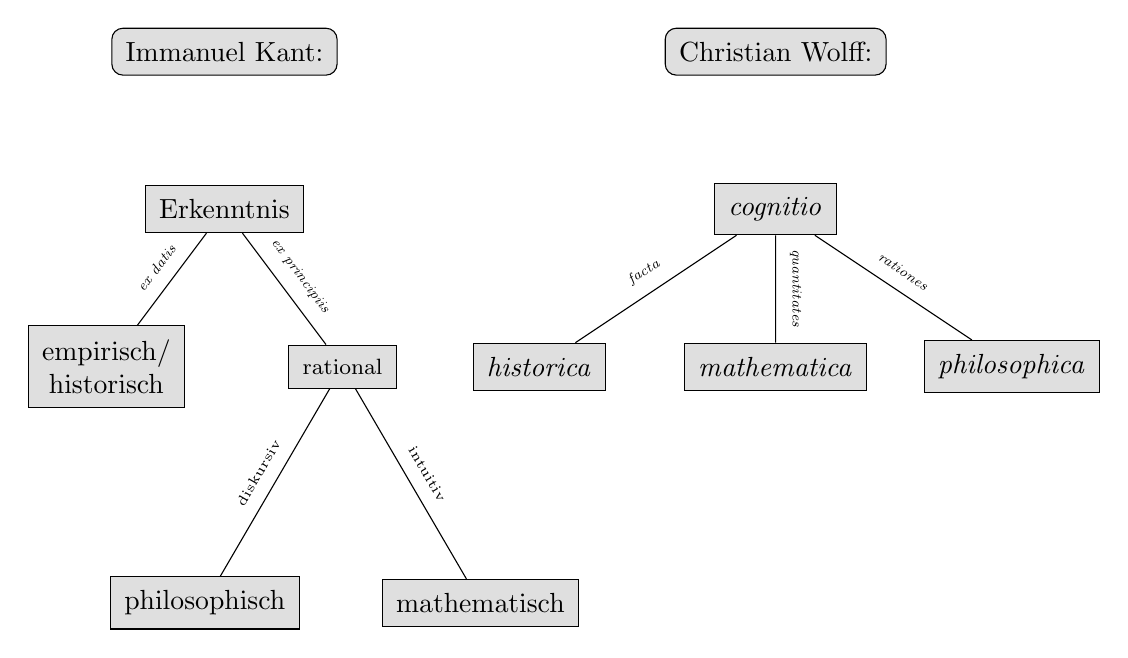
\begin{tikzpicture}[grow=down,%
%edge from parent fork down,
level 1/.style={sibling distance=7cm,level distance=0cm},
level 2/.style={sibling distance=7cm,level distance=2cm},
level 3/.style={sibling distance=3cm,level distance=2cm},
level 4/.style={sibling distance=3.5cm,level distance=3cm},
every node/.style={rectangle,draw=black,fill=gray!25, thin, inner sep=0.5em, minimum size=0.5em, align=center},
edge from parent/.style={draw},
mylabel/.style={draw=none, fill=none, text width=5cm,text centered, inner sep=0.5em, anchor=base} ]
\node[draw=none,fill=none] {}
child {node[rounded corners] {Immanuel Kant:} edge from
parent[draw=none] child {node {Erkenntnis} edge from parent[draw=none]
 child {node {empirisch/\\ historisch}
 		edge from parent node[draw=none,fill=none,above,sloped] {\tiny \emph{ex
 		datis}}} child {node {\footnotesize rational}
	child {node {philosophisch}
 		edge from parent node[draw=none,fill=none,above,sloped] {\tiny diskursiv}}
  	child {node (mathematisch) {mathematisch}
 		edge from parent node[draw=none,fill=none,above,sloped,text width=1.8cm]
 		{\tiny{intuitiv}}} edge from parent
 		node[draw=none,fill=none,above,sloped] {\tiny \emph{ex principiis}}}}}
child {node[rounded corners] {Christian Wolff:} edge from
parent[draw=none] child {node {\emph{cognitio}} edge from parent[draw=none]
 child {node {\emph{historica}}
 		edge from parent node[draw=none,fill=none,above,sloped] {\tiny \emph{facta}}}
 child {node {\emph{mathematica}}
 		edge from parent node[draw=none,fill=none,above,sloped] {\tiny \emph{quantitates}}}
 child {node {\emph{philosophica}}
 		edge from parent node[draw=none,fill=none,above,sloped] {\tiny
 		\emph{rationes}}}}} ;
\end{tikzpicture}
%\includegraphics{ErkenntnisartennachWolffundKant.pdf}
  \caption{Einteilung der Erkenntnisarten nach
  \authorcite{Wolff:Psychologiaempirica1968} und \name[Immanuel]{Kant} im
  Vergleich}\label{abbildung:ErkenntnisartennachWolffundKant.pdf}
\end{minipage}
\end{figure}

Im folgenden soll \name[Immanuel]{Kant}s Fassung
dieser Systematik erläutert werden in Kontrast zu und in Anlehnung an
\authorcite{Wolff:Psychologiaempirica1968}s Darstellung, der sie zumindest in
ihren groben Konturen noch immer entspricht (siehe Abbildung
\ref{abbildung:ErkenntnisartennachWolffundKant.pdf}). Ich beginne hierzu im
nächsten Abschnitt mit dem Begriff der rationalen Erkenntnis, der bei
\name[Immanuel]{Kant} gegenüber \authorcite{Wolff:Psychologiaempirica1968} neu
eingeführt wird (Kapitel
\ref{subsection:Vernunfterkenntnis:MathematikPhilosophie}). Dazu ist auch der
zugehörige Gegenbegriff der historischen oder empirischen Erkenntnis zu klären
(Kapitel \ref{subsection:HistorischeundempirischeErkenntnis}). Eigentliches Ziel
ist die Herausstellung des Begriffs und der Bedeutung philosophischer
Erkenntnis, die -- wie sich herausstellen wird -- auch aus methodischen Gründen
im Zentrum der Forderung nach epistemischer Autonomie steht.\footnote{Siehe
dazu Kap. \ref{section:MetaphysikausderPerspektivedesMenschen}, insb.
\ref{paragraph:facettendesmetaphysikbegriffs}, sowie
\ref{section:AutonomieundtestimonialesWissen}.} Den Unterschied zwischen
philosophischer und mathematischer Erkenntnis als Unterarten der rationalen
Erkenntnisse und die besondere Stellung der mathematischen Erkenntnis werde ich
in Kapitel \ref{subsubsection:EndlichesundUnendlichesErkennen} eingehender
beleuchten, um die besonderen Schwierigkeiten der philosophischen Erkenntnis zu
besprechen, die sich aus der Endlichkeit unseres Denkens ergeben.

\subsection{Vernunfterkenntnisse}\label{subsection:Vernunfterkenntnis:MathematikPhilosophie}
Eine Abweichung von \authorcite{Wolff:Psychologiaempirica1968} ist bereits bei
oberflächlicher Betrachtung sichtbar:
\name[Immanuel]{Kant} fasst die mathematische und philosophische Erkenntnis
zunächst zur rationalen Erkenntnis zusammen, um sie anschließend
wieder zu differenzieren. Dahinter jedoch steht eine grundlegende Neufassung der
Begriffe philosophischer und mathematischer Erkenntnis sowie ein gegenüber
\authorcite{Wolff:Discursuspraeliminarisdephilosophiaingenere1996}
abgewandelter Begriff der Vernunfterkenntnis. Gerade \name[Immanuel]{Kant}s
Begriff rationaler Erkenntnis wird im weiteren Verlauf wichtig für ein
Verständnis dessen, was es nach ihm heißt, mündig Informationen zu rezipieren.


\authorfullcite{Wolff:Psychologiaempirica1968} nennt eine Erkenntnis
mathematisch, wenn sie von Quantitäten handelt.\footnote{\cite[Vg.][\S~14]{Wolff:Discursuspraeliminarisdephilosophiaingenere1996}:
\enquote{Cognitio quantitatis rerum est ea, quam \ori{mathematicam}
appellamus.}} So verfügt derjenige über eine \emph{cognitio mathematica}, der
weiß, dass die Fallbeschleunigung auf der Erdoberfläsche im Schnitt etwa $9,81
\frac{m}{s^2}$ beträgt oder dass im Kühlschrank noch zwei Flaschen Schwarzbier
liegen. Diese Erkenntnisse sehen auf den ersten Blick wie \emph{cognitiones
historicae} aus, aber wegen ihres thematischen Bezugs auf Quantitäten werden sie
\enquote{\emph{mathematicae}} genannt. Ebenso hat derjenige eine \emph{cognitio
mathematica} und nicht \emph{philosophica}, der bei der Angabe der Gründe einer
Tatsache auch die involvierten Quantitäten ausgehend von den Angaben der bei den
Gründen vorhandenen Quantitäten mit berechnen kann. Wer also
nicht nur die Erdanziehung auf der Grundlage der Tatsache der Gravitation,
\emph{dass} sich schwere Körper gegenseitig anziehen, zu erklären weiß (und so
über eine \emph{cognitio philosophica} verfügt), sondern darüber hinaus auch
auch mittels einer Berechnung ausgehend von Radius und Masse der Erde und dem
\name[Isaac]{Newton}schen Gravitationsgesetz $ F_G = G \cdot \frac{m_1 \cdot
m_2}{r^2} $ erklären kann, warum die Fallbeschleunigung gerade besagte $9,81
\frac{m}{s^2}$ beträgt, verfügt über eine \emph{cognitio mathematica}. Diese
setzt freilich die \emph{cognitio philosophica} voraus und bekräftigt
diese.\footnote{Der größte Nutzen der \emph{cognitio mathematica} ist nach
\authorcite{Wolff:Psychologiaempirica1968} gerade darin zu sehen, dass sie die
enthaltene \emph{cognitio philosophica} mit größerer Gewissheit ausstattet, und
nicht etwa in dem Nutzen, den uns mathematische Zusammenhänge auf technischem
Gebiet bringen \parencite[vgl.][\S~27]{Wolff:Discursuspraeliminarisdephilosophiaingenere1996}.}


Grundlage der \emph{cognitio mathematica} kann somit sowohl die \emph{cognitio
historica} als auch die \emph{cognitio philosophica} sein; es hat mitunter gar
den Anschein, als handle es sich bei der \emph{cognitio mathematica} wahlweise
um eine \emph{cognitio historica} oder \emph{cognitio philosophica} von
Quantitäten, also gar nicht um eine Art \emph{neben} diesen, sondern um eine
jeweilige \emph{Unterart} derselben. Eine solche Begriffsbestimmung ist aber
unbefriedigend, wie auch \name[Immanuel]{Kant} bemängelt, der darauf hinweist,
dass die Philosophie auch von Quantitäten und die Mathematik auch von Qualitäten
handle.\footnote{\enquote{Übrigens handelt die
Philosophie eben sowohl von Größen, als die Mathematik, z.\,B. von der Totalität, der Unendlichkeit usw.
Die Mathematik beschäftiget sich auch mit dem Unterschiede der Linien und
Flächen, als Räumen, von verschiedener Qualität, mit der Kontinuität der
Ausdehnung, als einer Qualität derselben} \mkbibparens{\cite[][B
743]{Kant:KritikderreinenVernunft2003}, \cite[][III:
470.15--20]{Kant:GesammelteWerke1900ff.}}.} Deswegen sei es ein Fehler, den
Unterschied der Erkenntnisarten auf dieser Grundlage fassen zu wollen, statt die
Art des Erkennens als Ausgangspunkt zu wählen.



Die Thematik einer jeweiligen Erkenntnisart, das, \emph{wovon} Erkenntnisse
einer bestimmten Art handeln, falls dies einheitlich und klar bestimmt sein
sollte, ergebe sich erst hinterher auf der Grundlage von Definitionen, die sich
auf die \singlequote{Form} der jeweiligen Erkenntnis beziehen:
\begin{quote}
In dieser Form besteht also der wesentliche Unterschied dieser beiden Arten der
Vernunfterkenntnis, und beruhet nicht auf dem Unterschiede ihrer Materie, oder
Gegenstände. Diejenigen, welche Philosophie von Mathematik dadurch zu
unterscheiden vermeineten, daß sie von jener sagten, sie habe bloß die
\ori{Qualität}, diese aber nur die \ori{Quantität} zum Objekt, haben die Wirkung
für die Ursache genommen. Die Form der mathematischen Erkenntnis ist die
Ursache, daß diese lediglich auf Quanta gehen
kann.\footnote{\cite[][B 742]{Kant:KritikderreinenVernunft2003},
\cite[][III: 469.34--470.4]{Kant:GesammelteWerke1900ff.}.}
\end{quote}
Unter einer Erkenntnis versteht \name[Immanuel]{Kant} hier\footnote{Siehe
Anmerkung \ref{Anmerkung:ErkenntnisInZweierleiSinn} auf S.
\pageref{Anmerkung:ErkenntnisInZweierleiSinn}. In der \singlequote{Stufenleiter}
bestimmt \name[Immanuel]{Kant} die Erkenntnis abweichend als eine Vorstellung,
die mit Bewusstsein auf Objekte bezogen wird.
Dass es sich dabei aber um einen anderen Begriff handelt, der nur mit demselben
Wort belegt ist, wird daraus deutlich, dass sich Erkenntnisse in diesem Sinne in
Anschauungen und Begriffe unterteilen. Sie \emph{bestimmen} ein Objekt nicht,
sondern dienen dazu, dieses \emph{in Urteilen} zu bestimmen, also in
Erkenntnissen der anderen Art. Sie sind aber selbst keine Urteile, sondern nur
mögliche Bestandteile von Urteilen.} die \enquote{bestimmte[.] Beziehung
gegebener Vorstellungen auf ein Objekt.}\footnote{\cite[][B
137]{Kant:KritikderreinenVernunft2003}, \cite[][III:
111.17--18]{Kant:GesammelteWerke1900ff.}.} Wir erkennen einen Gegenstand -- etwa
\singlequote{dieses Buch} --, wenn wir Vorstellungen -- die Anschauung des
Buches und den Begriff der Farbe Grün -- auf diesen Gegenstand beziehen und ihn
dadurch näher Bestimmen: \enquote{Dieses Buch ist grün.} Dadurch bringen wir die
beiden Vorstellungen -- hier die Anschauung und den Begriff -- zur objektiven
Einheit der Apperzeption und fällen ein Urteil. Denn ein Urteil ist
\enquote{nichts anderes {\punkt}, als die Art, gegebene Erkenntnisse
[Anschauungen und Begriffe; A.\,G.] zur objektiven Einheit der Apperzeption zu
bringen.}\footnote{\cite[][B 141]{Kant:KritikderreinenVernunft2003},
\cite[][III: 114.7--8]{Kant:GesammelteWerke1900ff.}.} Die \singlequote{Form}
einer Erkenntnis ist dann anhand dieser Beziehung zu charakterisieren, also
anhand der Frage, \emph{wie} oder auf welcher Grundlage wir die Vorstellung zur
objektiven Einheit der Apperzeption bringen. Die grundlegende Unterscheidung, die \name[Immanuel]{Kant}
hier als relevant erachtet, ist: Wir können die Vorstellungen auf der Grundlage
von Erfahrung (\emph{a posteriori}) oder ohne diese Grundlage (\emph{a priori}) zur
Einheit bringen.\footnote{\cite[Vgl.][B
12\,f.,]{Kant:KritikderreinenVernunft2003}
\cite[][III: 35.1--36.5]{Kant:GesammelteWerke1900ff.}.} Und dies spiegelt sich
wieder in der Art und Weise, wie \name[Immanuel]{Kant} nicht erst mathematische
und philosophische, sondern bereits historische und rationale Erkenntnisse
differenziert. \enquote{Wenn ich von allem Inhalte
der Erkenntnis, objektiv betrachtet, abstrahiere, so ist alles Erkenntnis,
subjektiv, entweder historisch oder rational. Die historische Erkenntnis ist
cognitio ex datis, die rationale aber cognitio ex
principiis}\footnote{\cite[][B~863\,f.,]{Kant:KritikderreinenVernunft2003}
\cite[][III: 540.30--33]{Kant:GesammelteWerke1900ff.}.} Der Unterscheidungsgrund
liegt -- wie hier schon zu vermuten ist -- darin, ob eine Erkenntnis
ausschließlich der Spontaneität entstammt oder nur durch Rekurs auf Rezeptivität
möglich ist. Die rationale Erkenntnis ist -- so werde ich später zeigen -- eine
Erkenntnis des autonomen oberen Erkenntnisvermögens, die historische Erkenntnis
ist eine Erkenntnis des unteren Erkenntnisvermögens.\footnote{Siehe
dazu Kap. \ref{subsection:MetaphysikundAutonomie}.}




Statt ihres Gegenstandsbereichs ist bei \name[Immanuel]{Kant} also der Ursprung
oder die Art ihres \emph{Erwerbs} Ausgangspunkt der Differenzierung von
Erkenntnisarten. Dabei unterscheidet er das Empirische vom
Rationalen und historische von rationalen Erkenntnissen.\footnote{\cite[Vgl.][B
863\,f.,]{Kant:KritikderreinenVernunft2003} \cite[][III:
540.27--33]{Kant:GesammelteWerke1900ff.}.} Auf das nicht ganz einfache
Verhältnis des Empirischen zu den historischen Erkenntnissen werde ich gleich
eingehen,\footnote{Siehe Kapitel
\ref{subsection:HistorischeundempirischeErkenntnis}.} bis dahin werde ich das
Empirische unberücksichtigt lassen und mich ausschließlich dem Unterschied
zwischen historischen und rationalen Erkenntnissen widmen.


\name[Immanuel]{Kant} bestimmt den Unterschied historischer und
rationaler Erkenntnis folgendermaßen: Historische Erkenntnis ist \emph{cognitio
ex datis}, rationale Erkenntnis \emph{cognitio ex principiis}. Rational ist eine
Erkenntnis, wenn sie \enquote{aus allgemeinen Quellen der Vernunft, {\punkt}
d.\,i. aus Prinzipien}\footnote{\cite[][B
864\,f.,]{Kant:KritikderreinenVernunft2003} \cite[][III:
541.15--17]{Kant:GesammelteWerke1900ff.}.} erkannt wird. Aus Prinzipien
oder den allgemeinen Quellen der Vernunft -- und nicht \emph{ex datis} -- stammen wiederum Philosophie und Mathematik. Mathematische und philosophische Erkenntnis haben somit eine wichtige Gemeinsamkeit: Sie sind beide \emph{Vernunfterkenntnisse}, also Erkenntnisse,
für deren Erwerb wir keine Erfahrung benötigen, die uns nicht gegeben (\emph{ex
datis}) werden müssen, sondern die wir aus dem je eigenen Gebrauch der Vernunft
schöpfen können. Dabei gibt es zwei Arten, eine Erkenntnis aus Prinzipien zu
generieren, und nach diesen zwei Arten differenziert \name[Immanuel]{Kant} die beiden Arten
rationaler Erkenntnisse, Mathematik und Philosophie: Eine rationale Erkenntnis
ist eine \singlequote{\emph{diskursive}} Vernunfterkenntnis \emph{aus Begriffen}
oder eine \singlequote{\emph{intuitive}} Vernunfterkenntnis \emph{aus der
Konstruktion von Begriffen}. Vernunfterkenntnisse aus Begriffen sind
philosophische, Vernunfterkenntnisse aus der Konstruktion von Begriffen
mathematische
Erkenntnisse.\footnote{\enquote{Alle Vernunfterkenntnis ist nun entweder die
aus Begriffen, oder aus der Konstruktion von Begriffen; die erstere heißt
philosophisch, die zweite mathematisch} \mkbibparens{\cite[][B
865]{Kant:KritikderreinenVernunft2003},
\cite[][III: 541.18--20]{Kant:GesammelteWerke1900ff.}}.}



Damit ergibt sich die Einteilung, die im Ergebnis (ihrer resultierenden
Dreiteilung) derjenigen \authorcite{Wolff:Psychologiaempirica1968}s sehr ähnlich
sieht, insofern sie die Erkenntnisse in empirisch/historische (bei
\authorcite{Wolff:Psychologiaempirica1968}: \emph{cognitio historica}),
mathematische (bei \authorcite{Wolff:Psychologiaempirica1968}: \emph{cognitio
mathematica}) und philosophische Erkenntnisse (bei
\authorcite{Wolff:Psychologiaempirica1968}: \emph{cognitio philosophica})
einteilt (siehe wiederum
Abbildung \ref{abbildung:ErkenntnisartennachWolffundKant.pdf} auf Seite
\pageref{abbildung:ErkenntnisartennachWolffundKant.pdf}). In ihrem Konstruktionsprinzip hingegen unterscheidet sich diese
Einteilungen gewaltig voneinander, insofern
\authorcite{Wolff:Psychologiaempirica1968} die Erkenntnisse hinsichtlich ihres
Gegenstandes -- \emph{facta},
\emph{rationes}, \emph{quantitates} -- unterscheidet, \name[Immanuel]{Kant}
hingegen hinsichtlich der Art ihres Erwerbs -- \emph{ex datis}, \emph{ex
principiis}, aus Begriffen, aus der Konstruktion von Begriffen.

Der wichtigste Unterschied zwischen \name[Immanuel]{Kant}s und
\authorcite{Wolff:Psychologiaempirica1968}s Einteilung ist folgender:
\authorcite{Wolff:Psychologiaempirica1968} erklärt uns, dass \emph{jede} Erkenntnis ihre Grundlage
in der Erfahrung habe, denn die rationale Erkenntnis zeichnet sich nicht durch
die Quellen ihres ursprünglichen Erwerbs aus, sondern durch ihre rationale
\emph{Verbindung}.\footnote{\cite[Vgl.][\S~483]{Wolff:Psychologiaempirica1968}:
\enquote{\ori{Ratio} est facultas nexus veritatum universalium intuendi seu
perspiciendi.} \cite[Außerdem][\S\S~10\,f., 26,
34]{Wolff:Discursuspraeliminarisdephilosophiaingenere1996}.
\enquote{Praemittenda adeo est cognitioni philosophicae historica atquecum ista
constanter conjugenda, ne firmum desit fundamentum}
\parencite[][\S~11]{Wolff:Discursuspraeliminarisdephilosophiaingenere1996}.
Dabei zeigt \S~10, dass wir um die Gründe für eine Tatsache wiederum aus
Erfahrung wissen können und also historische Erkenntnis die feste Grundlage
(\enquote{firm[um] ac inconcuss[um] \punkt\ fundament[um]}, \S~11) der
philosophischen liefern kann. Zusätzlich ist die philosophische Erkenntnis der
Bestätigung durch historische Erkenntnis im Experiment bedürftig (\S~26).
Insofern die Philosophie Wissenschaft sein soll, muss sie nach \authorcite{Wolff:Psychologiaempirica1968} in
Experiment und Beobachtung fundiert sein: \enquote{In philosophia itaque
principia ab experientia derivanda, quae demonstrantur experimentis ac
observationibus confirmanda}
\parencite[][\S~34]{Wolff:Discursuspraeliminarisdephilosophiaingenere1996}.
\cite[Siehe
auch][\pno~44\,f.]{Schneiders:VernunftundVerstand--KriseneinesBegriffspaares1995}.}
Und diese Erfahrungsgebundenheit gelte nicht nur innerhalb der Naturforschung,
sondern auch für die \emph{philosophia prima}, Moral- und politische Philosophie
und sogar für die Mathematik, die ihre Begriffe, teilweise sogar ihre Grundsätze aus der Erfahrung
hätten.\footnote{\cite[Vgl.][\S~12]{Wolff:Discursuspraeliminarisdephilosophiaingenere1996}.}
Das Neue an \name[Immanuel]{Kant}s Systematik ist die Annahme eines Bereichs von Erkenntnissen, die ihre Quelle in der
Vernunft -- der \enquote{Spontaneität} als
Selbsttätigkeit\footnote{\enquote{Selbsttätigkeit} ist bei \name[Immanuel]{Kant}
wie schon bei
\authorcite{Baumgarten:Metaphysica---Metaphysik2011} die Übersetzung des lateinischen \enquote{spontaneitas}
\mkbibparens{\cite[vgl.][B~68]{Kant:KritikderreinenVernunft2003}, \cite[][III:
70.22, 70.27, 107.25]{Kant:GesammelteWerke1900ff.};
\cite[][\S~704]{Baumgarten:Metaphysica---Metaphysik2011}, auch in \cite[][XVII:
131.26, 131.33]{Kant:GesammelteWerke1900ff.}}. Noch
\authorcite{Wolff:Psychologiaempirica1968} übersetzt \enquote{spontaneitas} als
\enquote{Willkühr}, wie er im ersten Register der \enquote{Deutschen Metaphysik}
vermerkt
\parencite[vgl.][677]{Wolff:VernuenftigeGedankenvondenKraeftendesmenschlichenVerstandesundihremrichtigenGebraucheinErkenntnisderWahrheit1978}.}
des erkennenden Subjekts -- haben.



\subsection{\emph{Cognitio ex datis}: Historische und empirische
Erkenntnis}\label{subsection:HistorischeundempirischeErkenntnis}
Einen weiteren bereits oberflächlich erkennbaren Unterschied zwischen
\authorcite{Wolff:Psychologiaempirica1968}s und \name[Immanuel]{Kant}s
Systematik stellt die Verwendung des Wortes \enquote{empirisch} dar. Während
\authorcite{Wolff:Psychologiaempirica1968} zumindest im \titel{Discursus
praeliminaris} unisono von \emph{cognitiones historicae} spricht, verwendet
\name[Immanuel]{Kant} manchmal den Ausdruck \enquote{historisch} und mitunter
den Ausdruck \enquote{empirisch}, um eine Erkenntnis zu bezeichnen, die keine
Vernunfterkenntnis ist. Zunächst ließe sich vermuten, dass \enquote{empirisch}
einfach ein Synonym zu \enquote{historisch} ist; schon bei
\authorcite{Wolff:Discursuspraeliminarisdephilosophiaingenere1996} waren die
historischen Erkenntnisse mit den Erfahrungserkenntnissen zumindest
koextensional. Bei \name[Immanuel]{Kant} scheint sich bereits aus der
Begriffsbestimmung zu ergeben, dass genau die empirischen Erkenntnisse
historisch sind. Eine weitere sprachlich naheliegende Möglichkeit besagt, dass
wir unter empirischen Erkenntnissen die Erkenntnisse aus eigener Erfahrung,
unter historischen Erkenntnissen aber die uns mitgeteilten Erkenntnisse aus
zweiter Hand verstehen.\footnote{Dies schlägt
\authorfullcite{Kater:PolitikRechtGeschichte1999} vor
\parencite[vgl.][140]{Kater:PolitikRechtGeschichte1999}.} Beide Vorschläge
taugen nicht als Interpretation der Unterscheidung, wie ich in diesem Abschnitt
darlegen werde.


\authorfullcite{Kambartel:ErfahrungundStruktur1968}
behauptet, es sei zwischen der \emph{cognitio ex datis} als historischer
Erkenntnis auf der einen und empirischer Erkenntnis auf der anderen Seite scharf
zu unterscheiden, da \name[Immanuel]{Kant} mit der \emph{cognitio ex datis} im
Anschluss an \authorcite{Wolff:Psychologiaempirica1968} ausschließlich singuläre
Aussagen über einzelne Gegenstände und einzelne Geschehnisse
bezeichne\footnote{\authorcite{Kambartel:ErfahrungundStruktur1968}
sieht Allgemeines bei
\authorcite{Wolff:Discursuspraeliminarisdephilosophiaingenere1996} in
historischen Erkenntnissen nur in Form von \emph{Begriffen} enthalten. Wegen
deren Allgemeinheit brauche es auch für
\authorcite{Wolff:Psychologiaempirica1968} und alle anderen, die hierin in der
Tradition des \singlename{Aristoteles} stehen, mehrere Wahrnehmungen, um eine
Erfahrung bilden zu können
\parencite[Vgl.][55--57]{Kambartel:ErfahrungundStruktur1968}. Mit
\name[Immanuel]{Kant} gesprochen ließe sich sagen: Es müssen \emph{viele} Fälle
gegeben sein, damit wir mittels \textit{reflektierender} Urteilskraft Begriffe
\emph{bilden} können, die dann die \textit{bestimmende} Urteilskraft auf einen
einzelnen Fall \emph{anwenden} kann. Aber die \emph{Urteile} bleiben doch
singuläre.}, während empirische Erkenntnisse wesentlich allgemein seien oder
wesentlich allgemeine Behauptungen enthielten.\footnote{\cite[Vgl.][54--58, 85,
99]{Kambartel:ErfahrungundStruktur1968}.} \enquote{Von der \enquote{cognitio ex
datis} ist bei \name[Immanuel]{Kant} wie bei \name[Gottfried Wilhelm]{Leibniz}
die \enquote{empirische \ori{Erkenntnis}} wohl zu unterscheiden.
Diese, d.\,h.\ z.\,B.\ die Physik, ist Philosophie, nämlich \enquote{empirische
Philosophie}.}\footnote{\Cite[][85]{Kambartel:ErfahrungundStruktur1968}.
Interessant ist, dass \authorcite{Kambartel:ErfahrungundStruktur1968} den
Ausdruck \enquote{Erkenntnis} in Entgegensetzung gegen die \emph{cognitio ex
datis} betont, als ob es sich bei dieser nicht um eine Erkenntnis
handelte.} Während historische Erkenntnisse nur in singulären, nicht aber in
generellen Urteilen bestünden, verwende \name[Immanuel]{Kant}
\enquote{empirische Erkenntnis} gleichbedeutend mit der \enquote{rationale[n]
Verarbeitungsstufe der Wahrnehmung, die exemplarisch die physikalische
Erkenntnis
darstellt}\footnote{\Cite[][99]{Kambartel:ErfahrungundStruktur1968}.}.
In dieser Unterscheidung sieht \authorcite{Kambartel:ErfahrungundStruktur1968} die wichtige Neuerung, die
\name[Immanuel]{Kant}s Philosophie gegenüber ihren Vorläufern erbringe -- ein
besseres Verständnis des Empirischen, welches er dem bloß Historischen der
Neuzeit gegenüberstelle. Die Grundlage hierfür bestehe in den von
\name[Immanuel]{Kant} angeführten \emph{empirischen}
Prinzipien\footnote{\cite[Vgl.][85]{Kambartel:ErfahrungundStruktur1968}.}, so
dass die empirische Erkenntnis wegen ihrer in Prinzipien gründenden
Allgemeinheit auf die Seite der \emph{cognitio ex principiis} zu gehören scheint.

Dass zumindest ein Teil dieser Behauptungen nicht haltbar ist, zeigte bereits
das letzte Kapitel. Die Tradition, in der \name[Immanuel]{Kant} steht, versteht
unter der \emph{cognitio historica} keine singulären Urteile in dem Sinn, den
\authorcite{Kambartel:ErfahrungundStruktur1968} hier voraussetzt. Und auch
\name[Immanuel]{Kant} gibt -- soweit ich sehe -- keinerlei Anlässe, den Begriff
historischer Erkenntnis in diesem Sinne zu
fassen.\footnote{\name[Immanuel]{Kant} bringt den Begriff historischer
Erkenntnis nur im Kontrast zu \singlequote{dogmatischer} Erkenntnis mit dem
Mangel an Allgemeinheit in Verbindung, welcher ihr aber auch nur manchmal
anhafte. Eine solche Darstellung findet sich zumindest in der \titel{Logik
Blomberg}:
\leftquote Eine Erkenntniß ist \ori{Historisch}, wenn sie mit der Form der
Vernunft nicht übereinstimmet, \ori{rational} wenn sie mit derselben
übereinstimmet, und zwar ohne Ansehung des Objects. Hier aber müßen wir auch
auf das Object reflectiren, wenn wir den Unterschied zwischen der
Dogmatischen, und Historischen Erkenntniß feste setzen wollen.
\begin{enumerate}
  \item[1.\textsuperscript{mo}] Die \ori{Dogmatische} ist eine allgemeine
  Erkenntniß, die a priori aus der Vernunft entspringet
  \item[2.\textsuperscript{do}] Die \ori{Historische} aber ist \myemph{nicht
  immer} allgemein, und beruhet auf den aussagen geschehener Dinge, auf der
  aussage der anderen, sie entstehet also \ori{a posteriori}.\rightquote{}
  \mkbibparens{\cite{Kant:LogikBlomberg1966}, \cite[][XXIV:
99.14--24]{Kant:GesammelteWerke1900ff.}}\end{enumerate} Daraus scheint
  aber doch zu folgen, dass das Historische
  \emph{manchmal} allgemein ist.}
Fraglos handelt es sich bei Vernunfterkenntnissen ausnahmslos
um allgemeine Erkenntnisse und nicht um singuläre Aussagen. Wenn eine Aussage also ein
singuläres Urteil artikuliert, dann liegt notwendig eine historische Erkenntnis
vor. Aber daraus folgt nicht, dass alle historischen Erkenntnisse in singulären
Urteilen bestehen. Und noch viel weniger lässt sich daraus etwas über den
Unterschied zwischen historischen und empirischen Erkenntnissen lernen.
Empirischen Erkenntnissen kommt \enquote{nur angenommene und komparative
\ori{Allgemeinheit}}\footnote{\cite[][B 3]{Kant:KritikderreinenVernunft2003};
\cite[][III: 29.3--4]{Kant:GesammelteWerke1900ff.}.} im Unterschied zur strengen Allgemeinheit von
Vernunfterkenntnissen zu -- \name[Immanuel]{Kant} nennt sie auch
\enquote{empirische Allgemeinheit}\footnote{\cite[][B
4]{Kant:KritikderreinenVernunft2003}, \cite[][III:
29.9]{Kant:GesammelteWerke1900ff.}.}. Aber für die Annahme, historischer
Erkenntnis fehle nach \name[Immanuel]{Kant} auch diese Stufe an Allgemeinheit,
fehlt schlicht jegliche textbasierte Evidenz. Und auch für die Annahme,
empirische Erkenntnisse seien -- wie
\authorcite{Kambartel:ErfahrungundStruktur1968} schreibt -- als
\enquote{rationale
Verarbeitungsstufe}\footcite[][99]{Kambartel:ErfahrungundStruktur1968} zu
verstehen, sehe ich keine Grundlage in \name[Immanuel]{Kant}s Schriften.

Dagegen ist es \emph{prima facie} nicht abwegig, von empirischen Prinzipien zu
sprechen und \emph{a fortiori} physikalische Erkenntnisse, wie sie
\authorcite{Wolff:Psychologiaempirica1968} als philosophische Erkenntnisse
vorschwebten, als \emph{cognitiones ex principiis} anzusehen.
\name[Immanuel]{Kant} spricht oft von \enquote{empirischen Prinzipien} und sogar von \enquote{Vernunfterkenntnis aus empirischen
Prinzipien}, die er \enquote{empirische Philosophie}\footnote{\cite[][B
868]{Kant:KritikderreinenVernunft2003}, \cite[][III:
543.25--26]{Kant:GesammelteWerke1900ff.}.} nennt.
Und damit scheint die hier vorgelegte Deutung der Unterscheidung von
historischen und Vernunfterkenntnissen durchaus gefährdet zu sein, insofern ich
vorausgesetzt habe, dass es sich bei den Vernunfterkenntnissen oder
\emph{cognitiones ex principiis} um Erkenntnisse \emph{a priori} handelt. Was
also sind Prinzipien und was sind Erkenntnisse aus Prinzipien?

Erkenntnisse aus Prinzipien sind zunächst ganz allgemein solche, die wir mittels
eines Vernunftschlusses erhalten, der als Obersatz eine allgemeine Aussage
enthält, die \emph{in dieser Verwendung als Obersatz eines Vernunftschlusses}
\enquote{Prinzip} genannt wird. \name[Immanuel]{Kant} schreibt:
\begin{quote}
Ich würde daher
Erkenntnis aus Prinzipien diejenige nennen, da ich das Besondre im Allgemeinen durch Begriffe erkenne. So ist denn
ein jeder Vernunftschluß eine Form der Ableitung einer Erkenntnis aus einem
Prinzip. Denn der Obersatz gibt jederzeit einen Begriff, der da macht, daß
alles, was unter der Bedingung desselben subsumiert wird, aus ihm nach einem
Prinzip erkannt wird. Da nun jede allgemeine Erkenntnis zum Obersatze in einem
Vernunftschlusse dienen kann, \punkt\ so können diese denn auch, \myemph{in
Ansehung ihres möglichen Gebrauchs}, Prinzipien genannt werden.\footnote{\cite[][B
357]{Kant:KritikderreinenVernunft2003}, \cite[][III:
238.24--32]{Kant:GesammelteWerke1900ff.}, \myherv . Einen \emph{Vernunft}schluss
nennt \name[Immanuel]{Kant} einen Schluss mit mehr als einer Prämisse; der
Gegenbegriff ist der des \emph{Verstandes}schlusses \mkbibparens{\cite[vgl.][B
360]{Kant:KritikderreinenVernunft2003},
\cite[][III: 240.14--20]{Kant:GesammelteWerke1900ff.}}.}
\end{quote}
Es kann also eine jede allgemeine Aussage -- wenngleich dies eine uneigentliche
Redeweise ist -- auch Prinzip genannt werden. Ob eine allgemeine Aussage ein Prinzip ist, das ist
keine Frage ihrer Form, insofern diese isoliert von anderen Urteilen betrachtet
wird. Eine allgemeine Aussage ist dann ein Prinzip, wenn sie in einem
entsprechenden logischen Kontext steht. Ein Vorurteil ist entsprechend der
\titel{Logik} zufolge ein vorläufiges Urteil, welches als Prinzip oder Grundsatz
(beide Ausdrücke sind synonym) akzeptiert wird und dadurch unbegründete oder
Fehlurteile generiert.\footnote{\enquote{Vorurteile sind vorläufige Urteile,
\ori{in so ferne sie als Grundsätze angenommen werden}. -- Ein jedes Vorurteil
ist als ein Prinzip irriger Urteile anzusehen und aus Vorurteilen entspringen
nicht vorurteile, sondern irrige Urteile} \mkbibparens{\cite[][A
116]{Kant:ImmanuelKantsLogik1977}, \cite[][IX:
75.24--27]{Kant:GesammelteWerke1900ff.}}.}

Die entsprechende allgemeine Aussage können wir nach \name[Immanuel]{Kant} nun
aber aus der Vernunft oder aus der Erfahrung haben; und somit gibt es 
Vernunftprinzipien und eben auch empirische
Prinzipien.\footnote{\cite[Vgl.][B~868]{Kant:KritikderreinenVernunft2003},
\cite[][III: 543.24--26]{Kant:GesammelteWerke1900ff.}: \enquote{Alle Philosophie
aber ist entweder Erkenntnis aus reiner Vernunft, oder Vernunfterkenntnis aus
empirischen Prinzipien. Die erstere heißt reine, die zweite empirische
Philosophie.}} Im ersten Fall läge ein \enquote{realer Vernunftgebrauch}
zugrunde, in dem die Vernunft selbst unabhängig von jeder Erfahrung (Begriffe
und) Grundsätze aufstellt, im zweiten Fall handelte es sich nur um einen
logischen Vernunftgebrauch, in dem die Vernunft ihr gegebene allgemeine
Erkenntnisse miteinander verknüpft, ohne selbst auf den konkreten Inhalt bezogen
zu sein.\footnote{\cite[Vgl.][B 355]{Kant:KritikderreinenVernunft2003},
\cite[][III: 237.26--30]{Kant:GesammelteWerke1900ff.}.} Entsprechend bezeichnet
\name[Immanuel]{Kant} den Begriff \enquote{Prinzip} als zweideutig:
Eine allgemeine Aussage könne relativ zu ihrem Gebrauch ein Prinzip sein,
insofern sie den Obersatz eines Vernunftschlusses bildet, und sie könne
\enquote{an sich selbst} und ihrem \enquote{eigenen Ursprung nach} ein Prinzip
sein.\footnote{\Cite[Vgl.][B 356]{Kant:KritikderreinenVernunft2003},
\cite[][III: 238.12--15]{Kant:GesammelteWerke1900ff.}.} Nur letztere nennt er
\enquote{schlechthin Prinzipien}, während \enquote{alle allgemeine Sätze
überhaupt komparative Prinzipien heißen
können.}\footnote{\Cite[][B~358]{Kant:KritikderreinenVernunft2003}, \cite[][III:
359.7--8]{Kant:GesammelteWerke1900ff.}.} Im Architektonikkapitel der
\titel{Kritik der reinen Vernunft} scheint mir dann wiederum gar kein Zweifel
daran zu bestehen, dass \name[Immanuel]{Kant} Prinzipien im Sinne hat, die
gänzlich \emph{a priori} sind.\footnote{Ein weiteres Indiz findet sich zu Beginn
der \titel{Kritik der Urteilskraft} innerhalb der Einteilung des
\singlequote{Gebiets der Philosophie}:
\enquote{So weit Begriffe a priori ihre Anwendung haben, so weit reicht der
Gebrauch unseres Erkenntnisvermögens nach Prinzipien und mit ihm die
Philosophie} \mkbibparens{\cite[][xvi]{Kant:KritikderUrteilskraft2009},
\cite[][V: 174.3--5]{Kant:GesammelteWerke1900ff.}}.} Gerade um dies
herauszustellen bemüht er sich um mehrfache Abgrenzung der \enquote{reinen Philosophie} auch gegen die
\enquote{empirische Philosophie} und ihre \enquote{empirischen
Prinzipien}.\footnote{\enquote{Alle Philosophie aber ist entweder Erkenntnis aus
reiner Vernunft, oder Vernunfterkenntnis aus empirischen Prinzipien. Die erstere
heißt reine, die zweite empirische Philosophie} \mkbibparens{\cite[][B
868]{Kant:KritikderreinenVernunft2003}, \cite[][III:
543.24--26]{Kant:GesammelteWerke1900ff.}}.} Prinzipien im eigentlichen Sinn
dieses Wortes sind \emph{a priori}\footnote{In der \titel{Jäsche-Logik} heißt
es: \enquote{Wir haben die Vernunfterkenntnisse für Erkenntnisse aus Prinzipien
erklärt; und hieraus folgt: daß sie a priori sein müssen}
\mkbibparens{\cite[][A~21]{Kant:ImmanuelKantsLogik1977}, \cite[][IX:
22.33--34]{Kant:GesammelteWerke1900ff.}}.} und darin unterscheidet sich
\name[Immanuel]{Kant}s Begriff der \emph{cognitio ex principiis} von
\authorcite{Wolff:Psychologiaempirica1968}s Begriff der \emph{cognitio
philosophica}. Die empirischen Prinzipien, von denen \name[Immanuel]{Kant}
spricht sind in ihrer Verwendung Prinzipien, aber doch keine Erkenntnisse aus
Prinzipien, sondern gerade aus Erfahrung. Nun ist es möglich, etwas auf der
Grundlage solcher empirischer Prinzipien zu erkennen, was dann in gewisser
Hinsicht eine Erkenntnis \singlequote{\emph{aus} (empirischen) Prinzipien} ist.
So kann derjenige, der das Fundament seines Hauses untergräbt, aus empirischen
Prinzipien und damit in einer gewissen Hinsicht \emph{a priori} wissen, dass es
einstürzt.\footnote{\cite[Siehe hierzu][B 2]{Kant:KritikderreinenVernunft2003},
\cite[][III: 28.7--18]{Kant:GesammelteWerke1900ff.}.} Doch wie er es doch nicht
gänzlich \emph{a priori} wissen kann, so ist seine Erkenntnis auch nicht
gänzlich \emph{ex principiis}. Denn die empirischen Erkenntnisse, die er als
Prinzipien verwenden kann, müssen doch zunächst in der Erfahrung gegeben
(\emph{ex datis}) sein.

Eine alternative Deutung der Unterscheidung historischer und empirischer
Erkenntnis entwickelt \authorfullcite{Kater:PolitikRechtGeschichte1999}, der überdies
\name[Immanuel]{Kant}s Unterscheidung von objektiv und subjektiv betrachteten
Erkenntnissen berücksichtigt. Nach \authorcite{Kater:PolitikRechtGeschichte1999}
zeichnet sich die empirische Erkenntnis -- ebenso wie die rationale Erkenntnis
-- durch Objektivität aus, weil sie aus eigener Erfahrung -- die
rationale Erkenntnis aus eigener Vernunft -- entspringe. Die historische
Erkenntnis hingegen sei bloß mitgeteilt, wie \name[Immanuel]{Kant} der
\titel{Jäsche-Logik} zufolge die historische Gewissheit als abgeleitete
Gewissheit aus \emph{fremder} Erfahrung der Gewissheit aus \emph{eigener}
Erfahrung gegenüberstellt\footnote{\cite[Vgl.][A
107\,f.,]{Kant:ImmanuelKantsLogik1977}
\cite[][IX: 71.3--7]{Kant:GesammelteWerke1900ff.}. Man beachte jedoch, dass an
dieser Stelle zum einen von historischer \emph{Gewissheit}, nicht aber von
historischer \emph{Erkenntnis} gesprochen wird und dass zum anderen die
historische Gewissheit als abgeleitete \emph{empirische} (\enquote{derivative
empirica}) Gewissheit der empirischen Gewissheit \emph{per se} gar nicht
entgegengestellt, sondern der \emph{ursprünglichen} empirischen
(\enquote{originarie empirica}) Gewissheit gegenübergestellt und damit doch noch
immer als eine von zwei Formen empirischer Gewissheit betrachtet wird.}; und so
wird auch plausibel, warum es sowohl von empirischer als auch von rationaler
Erkenntnis wiederum historische Erkenntnis geben kann. Nach diesem Modell
unterscheidet \name[Immanuel]{Kant} also zunächst zwischen objektiver und (bloß)
subjektiver Erkenntnis und unterteilt die objektive Erkenntnis wiederum in
rationale Erkenntnis (eigener Vernunftgebrauch) und empirische Erkenntnis
(eigene Erfahrung).\footnote{\cite[Vgl.][141]{Kater:PolitikRechtGeschichte1999}:
\enquote{Ist der Ursprung der Erkenntnis objektiv, beruht sie also auf
unmittelbarer Sinneswahrnehmung oder eigener Vernunftanstrengung. Die Erkenntnis
subjektiven Ursprungs ist die je mitgeteilte Erkenntnis, und zwar unabhängig
davon, ob sie auf fremder Erfahrung beruht oder auf fremder Vernunft. Damit ist
sichergestellt, daß eine mitgeteilte Vernunfterkenntnis aus Sicht dessen, dem
sie mitgeteilt worden ist, keine Erkenntnis \ori{der} Vernunft darstellt.}}


Diese grundlegende Unterscheidung ließe sich auch auf \name[Immanuel]{Kant}s
Unterscheidung subjektiv und objektiv zureichenden Fürwahrhaltens und die
Bezeichnung des lediglich subjektiv, nicht aber objektiv zureichenden
Fürwahrhaltens als \emph{Glauben} sowie des sowohl subjektiv als auch objektiv
zureichenden Fürwahrhaltens als \emph{Wissen} beziehen.\footnote{\cite[Vgl.][B
850]{Kant:KritikderreinenVernunft2003}, \cite[][III:
532.36--533.5]{Kant:GesammelteWerke1900ff.}, sowie \cite[][A 98--107]{Kant:ImmanuelKantsLogik1977},
\cite[][IX: 65.33--70.31]{Kant:GesammelteWerke1900ff.}.} Da die Bezeichnung
testimonialer Erkenntnis als \enquote{historischer Glaube} im 18. Jahrhundert durchaus
verbreitet war, liegt es nahe, diese Unterscheidung auch in die Deutung des
Begriffs historischer Erkenntnis hinein zu
lesen.\footnote{\authorfullcite{Kater:PolitikRechtGeschichte1999} stellt diese
Verbindungen nicht her. Er bezieht den subjektiven Ursprung nicht auf ein bloß
subjektiv zureichendes Fürwahrhalten und erkennt auch, dass
\name[Immanuel]{Kant} keinen Unterschied bzgl. der Evidenz von Wahrnehmungs-
und testimonialem Wissen behauptet. Dennoch deutet
\authorcite{Kater:PolitikRechtGeschichte1999} den Begriff \enquote{historisch}
im Sinne von \enquote{testimonial} und behauptet, solcher Erkenntnis komme nach
\name[Immanuel]{Kant} nur ein subjektiver, aber kein objektiver Ursprung zu,
obwohl er selbst zuvor sieht, dass \name[Immanuel]{Kant} die mittelbare
Erfahrung wie jede andere Erfahrung auch ansieht und dem historischen allein das
\emph{a priori} erkennbare
entgegensetzt \parencite[siehe][140]{Kater:PolitikRechtGeschichte1999}.} Der
Begriff historischer Erkenntnis wird hier also im Sinne testimonialer Erkenntnis
gedeutet und als (bloß) subjektiv abgetan, hinterher aber durch Überlegungen zur
Bonität des Zeugen partiell
rehabilitiert.\footnote{\cite[Vgl.][143--146]{Kater:PolitikRechtGeschichte1999}.}


Dem widerspricht jedoch der Status, der testimonialen Erkenntnissen bei
\name[Immanuel]{Kant} zugeschrieben wird (siehe Kapitel
\ref{Absatz:AufklaerungundZugangsInternalismus}). \name[Immanuel]{Kant}
negiert jeden graduellen wie auch jeden qualitativen Unterschied zwischen dem
Fürwahrhalten auf Grund eigener Erfahrung und dem auf Grund fremder
Erfahrung.\footnote{\cite[Vgl.][A 103]{Kant:ImmanuelKantsLogik1977}, \cite[][IX:
69.2--4]{Kant:GesammelteWerke1900ff.}.} In der \titel{Jäsche-Logik}
wird die historische Gewissheit explizit unter der Rubrik \enquote{Wissen}
thematisiert.\footnote{\cite[Vgl.][A 108]{Kant:ImmanuelKantsLogik1977},
\cite[][IX: 71.6--7]{Kant:GesammelteWerke1900ff.}.} Auch in \titel{Was heißt:
sich im Denken orientieren?} wird gesagt, dass testimoniale Erkenntnisse völlig
zu Recht als Wissen bezeichnet werden.\footnote{\cite[Vgl.][A
319]{Kant:Washeisst:SichimDenkenorientieren?1977},
\cite[][VIII: 141.10--17]{Kant:GesammelteWerke1900ff.}.} Wissen ist aber ein
Fürwahrhalten, das subjektiv \emph{und objektiv} zureichend
ist.\footnote{\cite[Vgl.][B 850]{Kant:KritikderreinenVernunft2003},
\cite[][III: 533.4--5]{Kant:GesammelteWerke1900ff.}, sowie
\cite[][A 107]{Kant:ImmanuelKantsLogik1977},
\cite[][IX: 70.27--31]{Kant:GesammelteWerke1900ff.}.} Wenn historische
Erkenntnis also Wissen ist oder sein kann, dann kann sie nicht dadurch
charakterisiert werden, dass man sagt, sie sei eine nur subjektiv zureichende
Erkenntnis. Und auch die Deutung, sie sei nur subjektiven, nicht aber objektiven
Ursprungs, konfligiert mit der kategorischen Gleichstellung von Erkenntnissen
aus eigener und solchen aus fremder Erfahrung.


In der Tat finden wir bei \name[Immanuel]{Kant} zunächst eine grundlegende
Unterscheidung, die sich des Begriffspaares
\enquote{subjektiv}/\enquote{objektiv} bedient und die begriffliche
Unterscheidung zwischen historischen und empirischen Erkenntnissen erst
ermöglicht. Erst im Anschluss unterscheidet er  rationale von historischen sowie
rationale von empirischen Erkenntnissen -- und setzt in der \titel{Kritik der
reinen Vernunft} das Rationale dem Empirischen entgegen. Daraus folgt gerade
deswegen nicht die Identität des Empirischen und des Historischen, weil beide
Unterscheidungen auf verschiedenen \singlequote{Ebenen} liegen. Und eben diese
unterschiedlichen \singlequote{Ebenen} werden mit Hilfe der Ausdrücke
\enquote{subjektiv} und \enquote{objektiv} beschrieben. Den deutlichsten
Ausdruck findet dies in der {\jaeschelogik}:
\begin{quote}
 Man kann nämlich Erkenntnisse unterscheiden\\
 1) nach ihrem \ori{objektiven} Ursprunge, d.\,i.\ nach den Quellen, woraus eine
Erkenntnis allein möglich ist. In dieser Rücksicht sind alle Erkenntnisse
entweder \ori{rational} oder \ori{empirisch};\\
 2) nach ihrem \ori{subjektiven} Ursprunge, d.\,i.\ nach der Art, wie eine
Erkenntnis von den Menschen kann erworben werden. Aus diesem letztern
Gesichtspunkte betrachtet sind die Erkenntnisse entweder \ori{rational} oder
\ori{historisch}, sie mögen an sich entstanden sein, wie sie wollen. Es kann
also \ori{objektiv} etwas ein Vernunfterkenntnis sein, was \ori{subjektiv} doch
nur historisch ist.\footnote{\cite[][A~20f.,]{Kant:ImmanuelKantsLogik1977}
\cite[][IX: 22.11--20]{Kant:GesammelteWerke1900ff.}. Dies fügt sich auch sehr
gut in die -- weitaus weniger ausführlichen und daher deutungsoffeneren -- Ausführungen der ersten Kritik ein:
\enquote{Ich verstehe hier aber unter Vernunft das ganze obere
Erkenntnisvermögen, und setze also [objektiv betrachtet, A.\,G.] das Rationale
dem Empirischen entgegen.\\
 Wenn ich [hingegen; A.\,G.] von allem Inhalte der Erkenntnis, objektiv
betrachtet, abstrahiere, so ist alles Erkenntnis, subjektiv, entweder historisch
oder rational} (\cite[][B~863f.,]{Kant:KritikderreinenVernunft2003}
\cite[][III: 540.27--31]{Kant:GesammelteWerke1900ff.}).}
\end{quote}
Wir dürfen dies nicht so verstehen, dass einige Erkenntnisse einen objektiven,
andere lediglich einen subjektiven Ursprung hätten. \emph{Jede} Erkenntnis, die
als konkretes Wissen eines Subjekts von einem Sachverhalt vorliegt, kann sowohl
hinsichtlich ihres subjektiven als auch hinsichtlich ihres objektiven Ursprungs
betrachtet werden. Jede Erkenntnis hat folglich sowohl einen objektiven als auch
einen subjektiven Ursprung. Gerade \emph{nicht} unterschieden werden hier
subjektive von objektiven Erkenntnissen oder ein nur subjektiv zureichendes
Fürwahrhalten (Glauben) von einem solchen, das auch objektiv zureichend ist
(Wissen).

Eine Erkenntnis subjektiv betrachten heißt, auf das jeweilige
Verhältnis des Denkenden zu dieser Erkenntnis achten. Hierbei interessiert nicht
der Inhalt der Erkenntnis, sondern aus welchen Gründen jemand diese für wahr
hält. Sie ist dabei historisch, wenn sie in einem konkreten Fall für wahr
gehalten wird, weil die in Rede stehende Person selbst wahrgenommen oder von
anderen erfahren hat, dass etwas der Fall ist. Zwischen eigener und fremder Erfahrung existiert aus
\name[Immanuel]{Kant}s Perspektive kein relevanter Unterschied\footnote{Dies gilt für
seine publizierten Werke. In den Logikvorlesungen unterschied \name[Immanuel]{Kant} sehr
wohl zwischen eigener und fremder Erfahrung und auch zwischen Erfahrungen
erster, zweiter und dritter Hand und diskutiert auch die Frage, wie die
Glaubwürdigkeit sukzessiv abnimmt (bei \enquote{subordinirten Zeugen},
\enquote{mündliche Überlieferung}) oder durch das übereinstimmende Zeugnis
Vieler \enquote{coordinirte[r] Zeugen} (\enquote{das öffentliche Gerüchte})
zunimmt \mkbibparens{vgl. \cite{Kant:LogikPhilippi1966}, \cite[][XXIV:
450.20-28]{Kant:GesammelteWerke1900ff.}}.}, beides ist subjektiv betrachtet
historische Erkenntnis.

Eine Erkenntnis objektiv betrachten heißt hingegen, von dem
Verhältnis eines besonderen Subjekts zu ihr gerade absehen und
fragen: Was für eine Art von Erkenntnis liegt vor? Ebenso wie wir unter
\enquote{Wissenschaft} einerseits die Institution und das Gesamt an vorliegendem
Wissen und andererseits die je eigene Fähigkeit und Expertise verstehen
können,\footnote{Diese Unterscheidung spielt in der deutschen
Aufklärungsphilosophie durchaus eine Rolle. Als Belege können die bereits oben
angeführten Erläuterungen von
\authorcite{Stiebritz:ErlaeuterungderWolffschenVernuenfftigenGedanckenvonGottderWeltundderSeeledesMenschenauchallenDingenueberhaupt1999}
zu \authorcite{Wolff:Discursuspraeliminarisdephilosophiaingenere1996}s Logik
dienen
\mkbibparens{\cite[vgl.][\S~44]{Stiebritz:ErlaeuterungenderVernuenftigenGedanckenvondenKraefftendesmenschlichenVerstandesWolffs1977},
sowie oben Kapitel \ref{paragraph:wolffswarnung},
S.~\pageref{Anmerkung:StiebritzZuSubiectiveundObiective}}. Siehe als weiteren
Beleg \cite[][4]{Mendelssohn:UeberdieFrage:washeisstaufklaeren?2008}.} so können
wir \enquote{Erkenntnis} einerseits als objektiv vorliegenden Teil der Wissenschaft
und andererseits als mein je eigenes Urteil verstehen. Im ersten Fall
betrachten wir eine Erkenntnis objektiv, im zweiten Falle subjektiv. Und auch im
Falle objektiver Erkenntnisse lässt sich fragen: Handelt es sich um eine
Erkenntnis \emph{a priori}, eine Vernunfterkenntnis? Oder handelt es sich um
eine Behauptung, deren Wahrheit ausschließlich durch Rekurs auf (eigene oder
fremde) Sinneswahrnehmung auszumachen ist, also eine Erkenntnis \emph{a
posteriori}? Wir fragen dann nicht mehr, ob dieser oder jener etwas ohne Rekurs
auf Erfahrungen oder Mitteilungen erkannte, sondern ob die Erkenntnis selbst
derart ist, dass es \emph{möglich} und \emph{angemessen} ist, sie ohne Hilfe der
Wahrnehmung zu erkennen. Der Unterschied zwischen rationalen und empirischen
Erkenntnissen fällt also mit der Unterscheidung zwischen Erkenntnissen oder
Urteilen \emph{a priori} und \emph{a posteriori} zusammen, die ebenso nur das
Urteil an sich, nicht aber die besondere Situation und die zufälligen
Kompetenzen des gerade Urteilenden berücksichtigt.


Eine Erkenntnis, die subjektiv betrachtet rationale Erkenntnis sein kann, ist
immer auch objektiv betrachtet rationale Erkenntnis. Aber während es
nicht möglich ist, von objektiv empirischer Erkenntnis subjektiv rationale
Erkenntnis zu erlangen (man müsste aus reiner Vernunft erkennen, was nur
empirisch erkennbar ist), lässt sich doch subjektiv historische Erkenntnis von
objektiv rationalen Erkenntnissen erwerben, insbesondere indem man sich sagen
lässt, was andere rational erkannt haben.\footnote{\authorcite{Wolff:Psychologiaempirica1968}
thematisiert außerdem den Fall, dass wir mathematische Sätze anhand der
Erfahrung belegen
\parencite[vgl.][\S~19]{Wolff:Discursuspraeliminarisdephilosophiaingenere1996}.
Wir könnten beispielsweise den Satz des \singlename{Pythagoras} dadurch stützen
wollen, dass wir verschiedene rechtwinklige Dreiecke ausmessen und induktiv darauf schließen,
dass $a^2 + b^2 = c^2$ allgemein gilt. Ähnlich verhält es sich mit den
Beispielen, die \authorcite{Kripke:NameundNotwendigkeit1981} anführt.
Dieser vermengt in seiner Kritik an der Auffassung, die Klassen apriorischer und
empirischer Erkenntnisse seien disjunkt, beide Ebenen, insofern er durch das
Anführung von Erkenntnissen, die objektiv rational, aber subjektiv historisch
sind, die Möglichkeit gegeben sieht, empirische Erkenntnis mathematischer
Wahrheiten zu haben \parencite[vgl.][\pno
45\,ff.]{Kripke:NameundNotwendigkeit1981}.} \begin{figure}[htb]
\begin{minipage}[t]{\textwidth}
\centering
\begin{tikzpicture}[edge from parent fork down,
level 1/.style={level distance=1.5cm},
level 2/.style={level distance=2.5cm},
sibling distance=2.5cm,
every node/.style={rectangle,draw=black,fill=gray!25, thin, inner sep=0.5em, minimum size=0.5em, align=center},
edge from parent/.style={->,thick,draw},
mylabel/.style={draw=none, fill=none, text width=5cm,text centered, inner sep=0.5em, anchor=base} ]
\node {Erkenntnis}
	child {node (or) {rational}
		child {node (sr) {rational}} edge from parent[-,thin]}
	child {node[fill=none,draw=none] {(objektiv)} edge from parent[draw=none]
		child {node[fill=none,draw=none] {(subjektiv)} edge from
		parent[draw=none]}} child {node (oe) {empirisch}
		child {node (sh) {historisch}} edge from parent[-,thin]}
;
\draw [->,decorate,decoration={snake,post
length=1mm,amplitude=.4mm,segment length=2mm},thick] (or.south) to
(sh.north);
\end{tikzpicture}
  \caption{Objektive und subjektive Differenzierung von Erkenntnissen nach
  Immanuel
  \name[Immanuel]{Kant}}\label{abbildung:ZeichnungErkenntnisartennachKant.pdf}
\end{minipage}
\end{figure}
Eine graphische Übersicht dazu gibt Abbildung
\ref{abbildung:ZeichnungErkenntnisartennachKant.pdf}, in der der problematische
Fall einer historischen Erkenntnis von Vernunftwahrheiten hervorgehoben ist.
Wir verstehen damit auch die Aussage der {\jaeschelogik} besser, die ich
bereits weiter oben\footnote{Siehe Kapitel
\ref{Zitat:Kant:TestimonialesWissenVernunftErfahrung}, Seite
\pageref{Zitat:Kant:TestimonialesWissenVernunftErfahrung}.} anführte:
\begin{quote}
 Wenn wir in Dingen, die auf Erfahrungen und Zeugnissen beruhen, unsre
Erkenntnis auf das Ansehen andrer Personen bauen: so machen wir uns dadurch
keiner Vorurteile schuldig; denn in Sachen dieser Art muß, da wir nicht alles
selbst erfahren, und mit unserm eigenen Verstande umfassen können, das Ansehen
der Person die Grundlage unsrer Urteile sein. -- Wenn wir aber das Ansehen
anderer zum Grunde unsers Fürwahrhaltens in Absicht auf Vernunfterkenntnisse
machen: so nehmen wir diese Erkenntnisse auf bloßes Vorurteil
an.\footnote{\cite[][A~120]{Kant:ImmanuelKantsLogik1977}, \cite[][IX:
77.31--78.5]{Kant:GesammelteWerke1900ff.}.}
\end{quote}
Testimoniale Erkenntnis ist eine Unterart historischer Erkenntnisse und wer
testimoniales Wissen um die Vernunftwahrheiten hat, die ein anderer erkannte,
der hat historische Erkenntnis objektiv rationaler Erkenntnisse. Die
Grundforderung der Aufklärung wertet testimoniales Wissen bezüglich
rationaler Erkenntnisse ab, erlaubt sie aber bei empirischen Erkenntnissen. Ob
wir etwas aus eigener oder fremder \emph{Erfahrung} haben, das markiert aus
Sicht des \enquote{sapere aude!} keinen relevanten Unterschied, wohl aber, ob
wir etwas aus eigener oder fremder \emph{Vernunft} haben.

Mit der Kritik an der historischen Erkenntnis von
Vernunftwahrheiten schließt sich \name[Immanuel]{Kant}
\authorcite{Descartes:OeuvresdeDescartes1983}' Kritik an der
Büchergelehrsamkeit an, aus der keine echte Wissenschaft resultiere, weil sie
bloß den Erwerb historischer Kenntnisse beinhalte.\footnote{Siehe dazu Kapitel
\ref{subsection:DescartesKritikantestimonialemWissen}, insb. ab
S.~\pageref{Abschnitt:DescartesundhistorischeKenntnisse}.} Wie auch schon
\authorcite{Wolff:Discursuspraeliminarisdephilosophiaingenere1996} 
unterscheidet sich \name[Immanuel]{Kant} darin von
\authorcite{Descartes:OeuvresdeDescartes1983}, dass er den Begriff
der \singlequote{bloß historischen Kenntnis} ausführlich ausarbeitet und dabei
nicht historische Erkenntnisse \emph{per se} ablehnt, sondern nur solche von
(objektiv) philosophischen (oder allgemeiner: rationalen)
Erkenntnissen. Im Unterschied zu
\authorcite{Wolff:Discursuspraeliminarisdephilosophiaingenere1996} grenzt er
den Bereich der philosophischen Erkenntnisse auf die Erkenntnisse \emph{a
priori} ein, zu deren Rechtfertigung wir nicht auf Erfahrung verweisen müssen.
Damit ist es ein weitaus engerer Bereich, der für Fragen der Mündigkeit
relevant ist, als noch bei \authorcite{Wolff:Discursuspraeliminarisdephilosophiaingenere1996}.
Übernähme er dessen Konzeption ohne Änderung, so wäre nur derjenige schlechthin
aufgeklärt, der in allen Bereichen der Wissenschaft eigene Kompetenz besitzt. In der Tat aber ist der
Bereich dessen, was für Mündigkeit relevant ist, viel geringer. Es ist
plausibel zu sagen, dass auch derjenige mündig sein kann, der Aussagen der
Quantenmechanik oder der Allgemeinen Relativitätstheorie weder zu erläutern noch
zu begründen in der Lage ist, während es eine zwingende Voraussetzung von
Mündigkeit ist, in Fragen des moralisch Richtigen selbst kompetent urteilen zu
können. Fragen der Moral sind nicht nur der Form nach philosophische (also
diskursive Vernunft-) Erkenntnisse -- während quantenmechanisches Wissen
(zumindest überwiegend, vielleicht aber auch zur Gänze) empirisches Wissen
darstellt --; die Moral ist darüber hinaus auch von grundlegender Bedeutung für
das, was \name[Immanuel]{Kant} die Bestimmung des Menschen nennt (siehe Kapitel
\ref{chapter:AufklaerungundWissenschaft}), während wir dieser Bestimmung auch
dann selbstbestimmt folgen können, wenn wir über kein tiefgreifendes
physikalisches Wissen verfügen.

Nach \name[Immanuel]{Kant}s Aufklärungsprogrammatik ist es problematisch, von
philosophischen Erkenntnissen \emph{bloß} testimoniales Wissen zu haben, weil dadurch
das Selbstdenken durch bloßes \singlequote{Nachbilden} ersetzt
wird.\footnote{\cite[Vgl.][B 864]{Kant:KritikderreinenVernunft2003},
\cite[][III: 541.8]{Kant:GesammelteWerke1900ff.}. \name[Immanuel]{Kant} spricht
dort von dem \enquote{nachbildende[n] Vermögen}, welches \enquote{nicht das
erzeugende} ist.} Dies ist die primäre Konkretisierung des \enquote{Sapere
aude!}: Man soll nicht dasjenige, was aus dem je eigenen Gebrauch der Vernunft
erkannt werden kann, stattdessen als genuin testimoniales Wissen übernehmen,
also als Wissen, dessen Korrektheit man unabhängig von der Autorität eines
Anderen nicht beurteilen kann. Und darauf bezieht sich die an
\authorcite{Wolff:Psychologiaempirica1968} angelehnte Abneigung gegen eine bloß historische Erkenntnis philosophischen Wissens hinter \name[Immanuel]{Kant}s
Diktum, man könne und solle nicht Philosophie, sondern Philosophieren
lernen.\footnote{\cite[Vgl.][A~5]{Kant:NachrichtvonderEinrichtungseinerVorlesungenindemWinterhalbenjahrevon1765-17661900ff.},
\cite[][II: 306.30--32]{Kant:GesammelteWerke1900ff.}, sowie
\cite[][B~865]{Kant:KritikderreinenVernunft2003}, \cite[][III:
541.34--542.2]{Kant:GesammelteWerke1900ff.}. Siehe zur Vorgeschichte dieser
Redeweise die Überlegungen von Norbert
\textcite[][]{Hinske:UrspruenglicheEinsichtundVersteinerung1995}, der
ebenfalls
\authorfullcite{Wolff:Discursuspraeliminarisdephilosophiaingenere1996}s drei
Erkenntnisarten als wichtige Grundlage ausmacht
\parencite[vgl.][19--23]{Hinske:UrspruenglicheEinsichtundVersteinerung1995}.
Dass wir häufig und mit einer gewissen Notwendigkeit den Unterricht mit einer
solchen historischen Darstellung wissenschaftlicher Lehren beginnen, worauf erst
die Einübung in wissenschaftliche Techniken, das eigene Verstehen
wissenschaftlicher Theorien und die selbständige Teilnahme an
Forschungstätigkeiten folgt, ist möglicherweise Hintergrund der zunächst schwer
verständlichen Aussage: \enquote{In einer Wissenschaft \ori{wissen} wir oft nur
die \ori{Erkenntnisse}, aber nicht die dadurch
\ori{vorgestellten Sachen}; also kann es eine Wissenschaft von demjenigen geben,
wovon unsre Erkenntnis kein Wissen ist}
(\cite[][A~110]{Kant:ImmanuelKantsLogik1977}, \cite[][IX:
72.8--10]{Kant:GesammelteWerke1900ff.}).}

\name[Immanuel]{Kant} nennt ein System diskursiver Vernunfterkenntnisse auch
\emph{Metaphysik}\footnote{\enquote{[D]as System der reinen Vernunft
(Wissenschaft), die ganze (wahre sowohl als scheinbare) philosophische
Erkenntnis aus reiner Vernunft im systematischen Zusammenhange {\punkt} heißt
\ori{Metaphysik}} \mkbibparens{\cite[][869]{Kant:KritikderreinenVernunft2003},
\cite[][III: 543.29--544.2]{Kant:GesammelteWerke1900ff.}}.} und stellt damit --
ausgerechnet -- eine Disziplin in den Mittelpunkt seines Aufklärungsprogramms,
die eben durch die Aufklärung in Verruf geraten zu sein
scheint.\footnote{Dass Metaphysik nicht im Gegensatz zur Aufklärung stehen
muss, sondern gerade deren Anliegen sein kann, ist freilich bekannt.
\authorfullcite{Beiser:Kantsintellectualdevelopment1992} etwa schreibt:
\enquote{Only metaphysics, the young Kant believed, could rescue the
\ori{Aufklärung}'s faith in reason from the attacks of the Pietists. Only it could
provide a rational justification for our moral and religious beliefs, and thus a
middle path between skepticism and fideism}
\parencite[][30]{Beiser:Kantsintellectualdevelopment1992}. Gerade das Bemühen
um eine Religion nach Maßgabe der Vernunft motiviert metaphysische Bemühungen
\parencite[vgl.][]{Schmidt-Biggemann:MetaphysikalsProvokation2010}.
Gegen die Metaphysik wendet sich in der deutschen Aufklärungsphilosophie
insbesondere der Versuch von \name[Christian]{Thomasius}, den Einfluss der
Theologie auf die Jurisprudenz zurückzuweisen
\parencite[vgl.][602]{Hunter:ChristianThomasiusandtheDesacralizationofPhilosophy2000}.
Zu einer \singlequote{bürgerlichen} Aufklärung in dieser Traditionslinie siehe
\cite[][passim.]{Hunter:RivalEnlightenments2001}.} Dies überrascht, insofern
Metaphysik landläufig gerade nicht mit der Aufklärung in Verbindung gebracht
wird und \name[Immanuel]{Kant} sie mit der Vernunftkritik gerade zu überwinden
scheint. Doch zunächst handelt es sich nicht um die (positive) Aufforderung, Metaphysik
selbst zu betreiben, sondern um die (negative) Warnung, keine metaphysischen
Behauptungen von anderen zu übernehmen. Es ist ja denkbar, dass wir auf
Metaphysik auch weitestgehend verzichten können. Wir müssten sie dafür zunächst
als solche identifizieren und jede Übernahme metaphysischer Überzeugungen auf
der Grundlage von Mitteilungen verweigern. Ich werde im folgenden zunächst
\name[Immanuel]{Kant}s Begriff der Metaphysik skizzieren, damit überhaupt
feststeht, um welchen Themenbereich es der Aufklärungsforderung geht. Ich werde
dabei in mehreren Schritten vorgehen: Zum ersten ist der Begriff der Metaphysik zu konkretisieren und sein enges Verhältnis zum Begriff
der Philosophie darzulegen. Es wird sich zeigen, dass \name[Immanuel]{Kant}s
gegenüber seinen Vorgängern deutlich veränderter Metaphysikbegriff die
methodischen Überlegungen aus diesem Kapitel mit den inhaltlichen Überlegungen
in Kapitel \ref{chapter:AufklaerungundWissenschaft} verbindet.

\section{Selbstdenken als
Metaphysik}\label{section:MetaphysikausderPerspektivedesMenschen}

Ob \name[Immanuel]{Kant} als Metaphysiker zu lesen ist, gehört zu den
Fragestellungen, welche die \name[Immanuel]{Kant}forschung der ersten Hälfte des
20. Jahrhunderts prägten.\footnote{Siehe dazu den Überblick in
\cite{Funke:DieDiskussionumdiemetaphysischeKantinterpretation1976}.} Man kann
aber kaum behaupten, dass die Diskussion zu einem abschließenden Ergebnis
gekommen wäre, denn noch immer ist unklar, wie sich \name[Immanuel]{Kant}s
Philosophie zur Metaphysik verhält.\footnote{Siehe dazu das schon etwas ältere,
aber noch immer aktuelle Urteil von
\textcite[vgl.][372]{Walsh:KantandMetaphysics1976}.} Einige Interpreten sehen
das Problem darin, dass der Ausdruck \enquote{Metaphysik} bei
\name[Immanuel]{Kant} keine einheitliche Bedeutung
habe.\footnote{\cite[Vgl.
bspw.][\pno~26\,f.]{Beiser:Kantsintellectualdevelopment1992}.
\authorfullcite{Brandt:KantalsMetaphysiker1990} schreibt: \enquote{Ein wichtiges Ziel der folgenden Ausführungen ist es zu zeigen, daß eine Pauschalvorstellung von \ori{der} Metaphysik in \ori{der} Kantischen Philosophie nur die Kreation des
Interpreten sein kann -- in den Werken, die die Quelle unserer Erkenntnisse
bilden, läßt sich eine einheitliche Vorstellung von Metaphysik und von \ori{dem}
Problem \ori{der} Metaphysik nicht finden}
\parencite[][77]{Brandt:KantalsMetaphysiker1990}.}

Eine wichtige Rolle spielen möglicherweise diachrone Unterschiede in der
Auffassung \name[Immanuel]{Kant}s zu Begriff, Wesen und Möglichkeit von
Metaphysik. So nennt \authorfullcite{Beiser:Kantsintellectualdevelopment1992}
vier verschiedene Phasen der zeitlichen Entwicklung \name[Immanuel]{Kant}s, die
mit unterschiedlichen Positionen zur Frage nach Metaphysik verbunden
sind.\footnote{Er spricht von der \enquote{\emph{period of infatuation}} (1746--1759),
der \enquote{\emph{period of disillusionment}} (1760--1766), der \enquote{\emph{period of partial
reconciliation}} (1766--1772) und der \enquote{\emph{period of divorce}} (1772--1780)
\parencite[vgl.][26]{Beiser:Kantsintellectualdevelopment1992}.} Und
\authorfullcite{Foerster:KantsMetaphysikbegriff1987} spricht von drei
Metaphysikbegriffen bei \name[Immanuel]{Kant} -- \singlequote{vor-kritisch},
\singlequote{kritisch} und
\singlequote{nach-kritisch}.\footnote{\cite[Vgl.][]{Foerster:KantsMetaphysikbegriff1987}.}
Nun interessiert hier der \singlequote{kritische} Begriff von
Metaphysik, insofern dieser auf der vernunftkritischen Analyse
unserer Endlichkeit basiert (der \singlequote{vor-kritische}
Begriff also nicht thematisch ist und das \titel{Opus postumum}
in dieser Arbeit nicht besprochen werden soll).

Was ist das neue an einer \singlequote{kritischen Metaphysik}?
\name[Immanuel]{Kant}s Explikation des Begriffs klingt einfach: Eine Metaphysik
ist kritisch genau dann, wenn ihr eine Untersuchung über die Möglichkeit von
Metaphysik vorangeht; andernfalls heißt sie dogmatisch.\footnote{Dogmatismus ist
die \enquote{Anmaßung, mit einer reinen Erkenntnis aus Begriffen (der
philosophischen), nach Prinzipien, so wie sie die Vernunft längst im Gebrauche
hat, ohne Erkundigung der Art und des Rechts, womit sie dazu gelanget ist,
allein fortzukommen. Dogmatism ist also das dogmatische Verfahren der reinen
Vernunft, \ori{ohne vorangehende Kritik ihres eigenen Vermögens}}
\mkbibparens{\cite[][B xxxv]{Kant:KritikderreinenVernunft2003}, \cite[][III:
21.27--30 ]{Kant:GesammelteWerke1900ff.}}. Siehe auch
\cite[][B 7]{Kant:KritikderreinenVernunft2003},
\cite[][III: 31.7--12]{Kant:GesammelteWerke1900ff.}.} Die Vernunftkritik
wiederum lässt sich unschwer als eine Analyse unserer
Endlichkeit\footnote{Darauf insistiert besonders 
\authorfullcite{Heidegger:KantunddasProblemderMetaphysik1965}
\parencite[vgl.][\S~5 und
passim]{Heidegger:KantunddasProblemderMetaphysik1965}.} und verstehen. Wir sind
endlich, insofern unsere Spontaneität nur durch Rückgriff auf unsere
Sinnlichkeit die eigene Tätigkeit mit Gehalt und Weltbezug ausstatten kann. Kein
Gedanke kann einen Inhalt haben, ohne dass er sich direkt oder indirekt auf
unsere Erfahrungen bezieht; ein Denken ohne Rezeptivität wäre entsprechend ein
\enquote{frictionless spinning in the
void}\footnote{\cite[][11]{McDowell:MindandWorld1994}.} (siehe hierzu Kapitel
\ref{chapter:endlichkeitmenschlichendenkens}).
Deswegen müssen sich metaphysische Begriffe und Erkenntnisse mindestens dadurch auf Sinnlichkeit
beziehen, dass sie für \emph{mögliche} Erfahrungen gelten.
Dies wiederum hat Auswirkungen auf den Begriff von Metaphysik.


\authorcite{Beckmann:ZurTransformationvonMetaphysikdurchKritik1985}
unterscheidet vier verschiedene mögliche Auswirkungen der Kritik auf
Metaphysik:
\begin{quote}
Kritik kann versuchen, Metaphysik \punkt
 entweder zu ersetzen \punkt
 oder zu zersetzen \punkt
 oder allererst zu ermöglichen \punkt
 oder prinzipiell zu verändern.
Im ersten Fall steht Kritik der Metaphysik gegenüber in der
Beziehung der \ori{Substitution}, im zweiten Fall in der Beziehung der \ori{Destruktion}, im dritten Fall
in der Beziehung der \ori{Konstitution} und im vierten Fall schließlich in der
Beziehung der \ori{Transformation}[.]\footnote{\cite[][292]{Beckmann:ZurTransformationvonMetaphysikdurchKritik1985}.}
\end{quote}
Dabei versuche \name[Immanuel]{Kant}s Vernunftkritik, Metaphysik
allererst zu ermöglichen oder zu \emph{konstituieren}. Damit scheint sich an den Inhalten der
Metaphysik nicht viel zu ändern, außer dass möglicherweise \emph{weniger}
metaphysische Wahrheiten erkannt werden können, als man zuvor fälschlicher Weise
annahm. Dagegen sehen auch einige Interpreten eine fundamentale Änderung.
\authorfullcite{Hoeffe:EthikohneundmitMetaphysik2007} etwa behauptet, gemessen
an dem überlieferten Begriff von Metaphysik sei \name[Immanuel]{Kant}s
Transzendentalphilosophie gar nicht
metaphysisch.\footcite[Vgl.][\pno~416\,f.]{Hoeffe:EthikohneundmitMetaphysik2007}
\begin{comment}
Und als paradigmatisch für eine verbreitete Auffassung kann eine Behauptung
\authorfullcite{Schnaedelbach:WirKantianer2005}s gelten:
\begin{quote}
Hinter dem \singlequote{alles zermalmenden Kant}, der die herkömmliche Metaphysik in Grund
und Boden kritisiert, wird allzu leicht der Begründer einer kritischen
Metaphysik der Natur und der Sitten übersehen. Das Neue daran ist, dass diese
neue Metaphysik ohne Gottesbezug auszukommen versucht -- ein für die
metaphysische Tradition unfassbarer Gedanke. {\punkt} der rationalen Theologie
ging es ja nicht um Religion, sondern um die Existenz einer Instanz, die mit der
Einheit der Welt auch ihre Erkennbarkeit sichert; so schien Metaphysik nur
möglich zu sein in der Perspektive des Gottesstandpunktes. Nach Kant gibt es
Metaphysik nur nach menschlichem Maß, das heißt nach Maßgabe der menschlichen
Vernunft, und daran vermochte die philosophische Episode des \singlequote{deutschen
Idealismus}, der Kant nicht angehört, nichts zu
ändern.\footcite[][837]{Schnaedelbach:WirKantianer2005}
\end{quote}
\name[Immanuel]{Kant}s \singlequote{kritische} Metaphysik unterscheide sich also
darin von anderen, dass sie nicht auf eine Erkenntnis Gottes als Basis unserer
Geltungsansprüche zurückgreife. Während beispielsweise
\authorcite{Descartes:OeuvresdeDescartes1983} glaubt, zunächst die
Existenz Gottes beweisen zu müssen, auf dieser Grundlage dann aber zeigen zu
können, dass alles, was wir klar und deutlich einsehen, unzweifelhaft wahr sein
müsse, verwerfe \name[Immanuel]{Kant} gerade den Gedanken einer solchen
\singlequote{metaphysischen} Fundierung. Damit entfalle aber auch die
gedankliche Möglichkeit eines Wissens \emph{sub specie aeternitatis}, eines
absoluten Wissens. Die Endlichkeit unseres Erkennens lässt sich demnach nicht
mehr durch metaphysische Überlegungen überwinden.
\end{comment}

Dies zeigt zur Genüge, dass der Metaphysikbegriff klärungsbedürftig ist, soll
die These von ihrem zentralen Stellenwert für die Forderung der Aufklärung nach
Mündigkeit gehaltvoll sein. Ich werde im folgenden zunächst
\name[Immanuel]{Kant}s Metaphysikbegriff rekonstruieren und sein Verhältnis zum Begriff
der Philosophie beleuchten (Kapitel \ref{paragraph:facettendesmetaphysikbegriffs}),
um anschließend zu zeigen, warum \name[Immanuel]{Kant} denkt, dass wir auf
Metaphysik nicht verzichten können (Kapitel
\ref{paragraph:DieUnverzichtbarkeitderMetaphysik}). Am Ende werde ich dann
zeigen, dass autonomes Denken tatsächlich darin besteht, \Revision{über
Kompetenz im Bereich der Metaphysik zu verfügen} (Kapitel
\ref{subsection:MetaphysikundAutonomie}). Freilich heißt dies nicht,
\Revision{über eine \singlequote{eigene} Metaphysik zu verfügen, die
  sich möglicherweise durch Originalität auszeichnen und sich von
derjenigen anderer unterscheiden soll.} Wir sollen im Bereich der einen
Metaphysik je selbst kompetent urteilen können.

\subsection{Kants
Metaphysikbegriff}\label{paragraph:facettendesmetaphysikbegriffs} Die
Philosophie der Neuzeit kennt keinen einheitlichen Metaphysikbegriff, sondern
vielfältige Verwendungsweisen von \enquote{Metaphysik} und
\enquote{metaphysisch}, die sich in synchroner Betrachtung zwischen den
Regionen, Strömungen und auch Autoren beträchtlich unterscheiden und in
diachroner Betrachtung den Wandlungen einer im Entstehen begriffenen
philosophischen Disziplin
unterliegen.\footnote{\cite[Vgl.][]{Borsche:ArtikelMetaphysikVI.Neuzeit1980}.}
Man beachte etwa, dass das bekannte Schema einer in Ontologie, rationale
Kosmologie, rationale Psychologie und rationale oder natürliche Theologie
einzuteilenden Metaphysik erst innerhalb der an
\authorcite{Wolff:Psychologiaempirica1968} anschließenden Schulmetaphysik entstand und die (terminologisch
fixierte) Einteilung in eine \textit{metaphysica generalis} und eine
\textit{metaphysica specialis} sogar noch jüngeren Datums
ist.\footnote{\authorfullcite{Vollrath:DieGliederungderMetaphysikineineMetaphysicaGeneralisundeineMetaphysicaSpecialis1962}
bemerkt, dass sich die Einteilung in eine allgemeine und eine spezielle
Metaphysik in der Philosophie vor \name[Immanuel]{Kant} gar nicht explizit,
sondern höchstens implizit finde
\parencite[vgl.][258--263]{Vollrath:DieGliederungderMetaphysikineineMetaphysicaGeneralisundeineMetaphysicaSpecialis1962}.
\authorfullcite{Albrecht:ChristianWolffundderWolffianismus2014} schreibt,
\authorcite{Wolff:Discursuspraeliminarisdephilosophiaingenere1996} habe diese
Unterscheidung von seinen Vorgängern nicht übernommen
\parencite[vgl.][105]{Albrecht:ChristianWolffundderWolffianismus2014}, wobei er
die Antwort auf die Frage schuldig bleibt, bei welchen Vorgängern die
Unterscheidung explizit getroffen wurde. Am nächsten kommt der Bezeichnung
\enquote{\emph{metaphysica generalis}} noch Alexander
\authorcite{Baumgarten:Metaphysica---Metaphysik2011}, der in seiner Metaphysik
-- und dort auch nur beiläufig im Sinne einer auch möglichen Bezeichnungsweise
-- von der Ontologie als einer \enquote{metaphysica universalis} spricht:
\enquote{\ori{Ontologia} (ontosophia, metaphysica, \punkt\ \myemph{metaphysica
universalis}, architectonica, philosophia prima,) est scientia praedicatorum
entis generaliorum}
\mkbibparens{\cite[][\S~4]{Baumgarten:Metaphysica---Metaphysik2011},
\cite[][XVII: 24.5--6]{Kant:GesammelteWerke1900ff.}}. Üblicher war es, die
Ontologie gar nicht als Metaphysik, sondern als \textit{prima philosophia} zu
bezeichnen \parencite[z.\,B.][]{Wolff:Philosophiaprimasiveontologia1977}.}
Der Begriff der Metaphysik schillert nicht minder als der der Aufklärung, weswegen die These, es
stünde gerade die Metaphysik im Zentrum der Aufklärung, erläuterungsbedürftig
ist.

\name[Immanuel]{Kant} gibt in der \titel{Kritik der reinen Vernunft}
verschiedene Bestimmungen des Metaphysikbegriffs an und unterscheidet mehrfach zwischen weiteren und engeren
Wortverwendungen.\footnote{\cite[Vgl.][B
869\,f.,]{Kant:KritikderreinenVernunft2003} \cite[][III:
543.27--544.24]{Kant:GesammelteWerke1900ff.}.} Die folgende Systematisierung,
bei der die Metaphysik bezüglich ihrer \textit{Quellen}
(\ref{MethodikundQuellenderMetaphysik}), ihrer \textit{Teildisziplinen}
(\ref{TeilDisziplinenDerMetaphysik}) und ihres \textit{Interesses}
(\ref{InteresseDerMetaphysik}) betrachtet wird, mag dabei zu einem besseren
Überblick beitragen und die Fragen nach Einheitlichkeit und Wahl der relevanten
Begriffsbestimmung zu beantworten.\footnote{In den \titel{Prolegomena}
betrachtet \name[Immanuel]{Kant} selbst die Metaphysik nach ihrem Objekt, ihren
Quellen und der Erkenntnisart. Die Erkenntnis\emph{art} betrifft in diesem
Zusammenhang die Unterscheidung synthetischer und analytischer Urteile.
\name[Immanuel]{Kant} betont diese Unterscheidung, weil eine Verwechslung zu
einem Irrtum über die eigentlichen \emph{Quellen} der Metaphysik führe. Denn zu
glauben, die Sätze der Metaphysik folgten aus dem Satz vom ausgeschlossenen
Widerspruch (seien also analytisch), heiße fälschlich die Quellen der
Metaphysik in ihr selbst, nicht in der reinen Vernunft suchen
\mkbibparens{\cite[vgl.][\S~3]{Kant:ProlegomenazueinerjedenkuenftigenMetaphysikdiealsWissenschaftwirdauftretenkoennen1977},
\cite[][IV: 270.5--15]{Kant:GesammelteWerke1900ff.}}. Die Betrachtung des
Objekts der Metaphysik entspricht wiederum der Betrachtung der Teildisziplinen.}
\begin{nummerierung}
\item\label{MethodikundQuellenderMetaphysik} In Bezug
auf ihre \emph{Erkenntnisquellen} wird Metaphysik als die Erkenntnis aus reiner
Vernunft
bestimmt.\footnote{\cite[Vgl.][\S~1]{Kant:ProlegomenazueinerjedenkuenftigenMetaphysikdiealsWissenschaftwirdauftretenkoennen1977},
\cite[][IV: 265.5--266.8]{Kant:GesammelteWerke1900ff.};
\cite[][B 869]{Kant:KritikderreinenVernunft2003},
\cite[][III: 543.27--544.2]{Kant:GesammelteWerke1900ff.}.}
\enquote{Metaphysische Erkenntnis muß lauter Urteile a priori enthalten, das erfordert das Eigentümliche ihrer Quellen.}\footnote{\cite[][\S~2]{Kant:ProlegomenazueinerjedenkuenftigenMetaphysikdiealsWissenschaftwirdauftretenkoennen1977}, \cite[][IV: 266.15--16]{Kant:GesammelteWerke1900ff.}.} Das ist die Bestimmung, der zufolge die Metaphysik den Überlegungen im vorangehenden Kapitel \ref{section:MuendigkeitundPhilosophie} zufolge im Fokus der Aufklärung steht.
Allerdings gibt es zwei Disziplinen, die gänzlich a priori erkennen: Philosophie und Mathematik.
Nun bestimmt \name[Immanuel]{Kant} eine Erkenntnis als mathematisch oder als
\emph{intuitive} rationale Erkenntnis, wenn sie aus der \emph{Konstruktion} von
Begriffen in der reinen Anschauung des Raumes (Geometrie) oder der Zeit
(Arithmetik) erfolgt. Diejenige apriorische Erkenntnis hingegen, die nicht durch
die Konstruktion von Begriffen erfolgt, nennt \name[Immanuel]{Kant}
philosophisch oder auch \emph{diskursive} rationale Erkenntnis. Und das System
der philosophischen Erkenntnisse oder der diskursiven Vernunfterkenntnisse heißt
Metaphysik.\footnote{\cite[Vgl.][B 869]{Kant:KritikderreinenVernunft2003}, \cite[][III: 543.27--544.2]{Kant:GesammelteWerke1900ff.}.} Dies ist die weiteste
und systematisch ursprüngliche unter den Bestimmungen, die \name[Immanuel]{Kant}
angibt. Daraus ergibt sich weiter, dass Metaphysik
schon begrifflich mit der (reinen) Philosophie
zusammenfällt,\footnote{\cite[Vgl.][B~869,
878]{Kant:KritikderreinenVernunft2003}, \cite[][III: 544.2--8,
549.13--16]{Kant:GesammelteWerke1900ff.}.} insofern sie die
Ver\-nunft\-er\-kennt\-nis aus Begriffen (nicht: aus der Konstruktion der
Begriffe) ist\footnote{\cite[Vgl.][B 865]{Kant:KritikderreinenVernunft2003}, \cite[][III:
541.18--20, 542.3]{Kant:GesammelteWerke1900ff.}.}.

Dabei ist sich \name[Immanuel]{Kant} der Tatsache bewusst, einen gegenüber den ihm stets präsenten
Vorgängern \authorcite{Wolff:Psychologiaempirica1968} und
\authorcite{Baumgarten:Metaphysica---Metaphysik2011} \textit{neuen}
Ausgangspunkt der Bestimmung des Metaphysikbegriffs zu wählen, indem er
festlegt, Metaphysik sei das, was wir aus reiner Vernunft
wissen. \authorcite{Wolff:Discursuspraeliminarisdephilosophiaingenere1996}
bestimmt die Metaphysik über Ihre Teilbereiche Ontologie, Kosmologie und
Pneumatik (Psychologie und natürliche
Theologie).\footcite[Vgl.][\S~79]{Wolff:Discursuspraeliminarisdephilosophiaingenere1996}
\authorcite{Baumgarten:Metaphysica---Metaphysik2011} definiert die Metaphysik
über ihre Stellung im System der Wissenschaften, ohne auf den Ursprung
metaphysischer Erkenntnis in der Vernunft oder der Erfahrung zu rekurrieren.
Eine Disziplin zählt nach ihm zur Metaphysik, wenn sie die Grundlage einer
Reihe anderer Disziplinen
bildet.\footnote{\label{Anmerkung:SchulmetaphysikMitEmpirischerPsychologie}\enquote{\ori{Metaphysica}
est scientia primorum in humana cognitione principiorum}
\mkbibparens{\cite[][\S~1]{Baumgarten:Metaphysica---Metaphysik2011},
\cite[][XVII: 23.16]{Kant:GesammelteWerke1900ff.}}. Dass dies nicht im Sinne
der obersten (apriorischen) Grundsätze \name[Immanuel]{Kant}s zu verstehen ist,
erhellt aus der Integration der empirischen Psychologie in die Metaphysik
\mkbibparens{\cite[vgl.][\S\S~502\,f.,]{Baumgarten:Metaphysica---Metaphysik2011}
\cite[][XVII: 130.17--22]{Kant:GesammelteWerke1900ff.}}.} Beide integrieren
daher auch bedenkenlos empirische Wissenschaften in die
Metaphysik; \authorcite{Wolff:Discursuspraeliminarisdephilosophiaingenere1996}
sieht sogar die empirische Psychologie gerade wegen ihres empirischen Charakters als
besonders geeignet an, eine tragende Rolle für andere Disziplinen zu
spielen.\footnote{\cite[Vgl.][\S~112]{Wolff:Discursuspraeliminarisdephilosophiaingenere1996}.}
Und auch \authorcite{Baumgarten:Metaphysica---Metaphysik2011} folgt
\authorcite{Wolff:Discursuspraeliminarisdephilosophiaingenere1996} in der
Integration der empirischen Psychologie in die Metaphysik,\footnote{Die
Abschnitte der \titel{Metaphysica}, die die empirische Psychologie behandeln,
wurden von \name[Immanuel]{Kant} der pragmatischen Anthropologie, wie er sie in
seinen Vorlesungen behandelte, zugrunde gelegt
\parencite[vgl.][\pno~54\,f.]{Falduto:TheFacultiesoftheHumanMindandtheCaseofMoralFeelinginKantsPhilosophy2014}.
Sie sind abgedruckt in Band XV der Akademieausgabe der Werke
\name[Immanuel]{Kant}s \parencite[siehe][XV:
5--54]{Kant:GesammelteWerke1900ff.}.} betrachtet Metaphysik also nicht als reine
Vernunftwissenschaft in einem Sinn, der \name[Immanuel]{Kant}s Metaphysikbegriff
bestimmt.

Hatte sich \name[Immanuel]{Kant} in früheren Schriften noch
\authorcite{Baumgarten:Metaphysica---Metaphysik2011}s Bestimmung des
Metaphysikbegriffs angeschlossen\footnote{\enquote{Die Metaphysik ist nichts
anders als eine Philosophie über die ersten Gründe unseres Erkenntnisses}
\mkbibparens{\cite[][A
79]{Kant:UntersuchungueberdieDeutlichkeitderGrundsaetzedernatuerlichenTheologieundderMoral1977},
\cite[][II: 283.13--14]{Kant:GesammelteWerke1900ff.}}. Offensichtlich handelt es
sich um eine Übersetzung der Definition
\authorcite{Baumgarten:Metaphysica---Metaphysik2011}s (siehe Anm. \ref{Anmerkung:SchulmetaphysikMitEmpirischerPsychologie}).}
und ebenfalls die empirische Psychologie zur Metaphysik gezählt\footnote{In den
1760er Jahren nennt er sie \enquote{die metaphysische Erfahrungswissenschaft vom
\ori{Menschen}} \mkbibparens{\cite[][A
9]{Kant:NachrichtvonderEinrichtungseinerVorlesungenindemWinterhalbenjahrevon1765-17661900ff.},
\cite[][II: 309.2--3]{Kant:GesammelteWerke1900ff.}}.}, so behauptet er in der
\titel{Kritik der reinen Vernunft}, nur durch die Neubestimmung die Metaphysik
als \emph{einheitliche} philosophische Disziplin begründen zu können:
\enquote{Alle reine Erkenntnis a priori macht also, vermöge des besonderen
Erkenntnisvermögens, darin es allein seinen Sitz haben kann, eine besondere
Einheit aus, und Metaphysik ist diejenige Philosophie, welche jene Erkenntnis in
dieser systematischen Einheit darstellen
soll}\footnote{\cite[][B~873]{Kant:KritikderreinenVernunft2003}, \cite[][III:
546.8--11]{Kant:GesammelteWerke1900ff.}.
\authorfullcite{Heidegger:KantunddasProblemderMetaphysik1965} behauptet, damit
entferne sich \name[Immanuel]{Kant} gar nicht von
\authorcite{Baumgarten:Metaphysica---Metaphysik2011}s Begriff der Metaphysik
\parencite[vgl.][\S~1]{Heidegger:KantunddasProblemderMetaphysik1965}.}.
\name[Immanuel]{Kant} behauptet, als erster eine klare Bestimmung der alten Idee einer Wissenschaft unter dem Namen
\enquote{Metaphysik} angegeben zu haben, indem er die Wissenschaften \emph{ihren
Quellen} und nicht ihren Objekten nach einteilt.\footnote{\cite[Vgl.][B
870--873]{Kant:KritikderreinenVernunft2003}, \cite[][III:
544.25--546.15]{Kant:GesammelteWerke1900ff.}.}
%
%
\item\label{TeilDisziplinenDerMetaphysik} \textit{Inhaltlich} oder in Bezug auf
ihre \emph{Teildisziplinen} weist \name[Immanuel]{Kant} der Metaphysik im
engeren Sinne folgende Themenfelder zu:
Ontologie, rationale Physiologie (unterteilt in \emph{physica rationalis} und
\emph{psychologia rationalis}), rationale Kosmologie und rationale Theologie. In einem
weiteren Sinne enthält sie außerdem die Kritik der reinen Vernunft als
Propädeutik und die Metaphysik der Sitten. Diese Inhalte ergeben sich aber nicht
rhapsodisch, sondern werden aus der methodischen Bestimmung als
Vernunfterkenntnis aus Begriffen entwickelt, wie Abbildung
\ref{abbildung:metaphysikeinteilung}
(auf Seite \pageref{abbildung:metaphysikeinteilung}) illustriert.
\begin{figure}[htb]
\begin{minipage}[t]{\textwidth}
\centering
% \includegraphics{Metaphysikeinteilung.pdf}
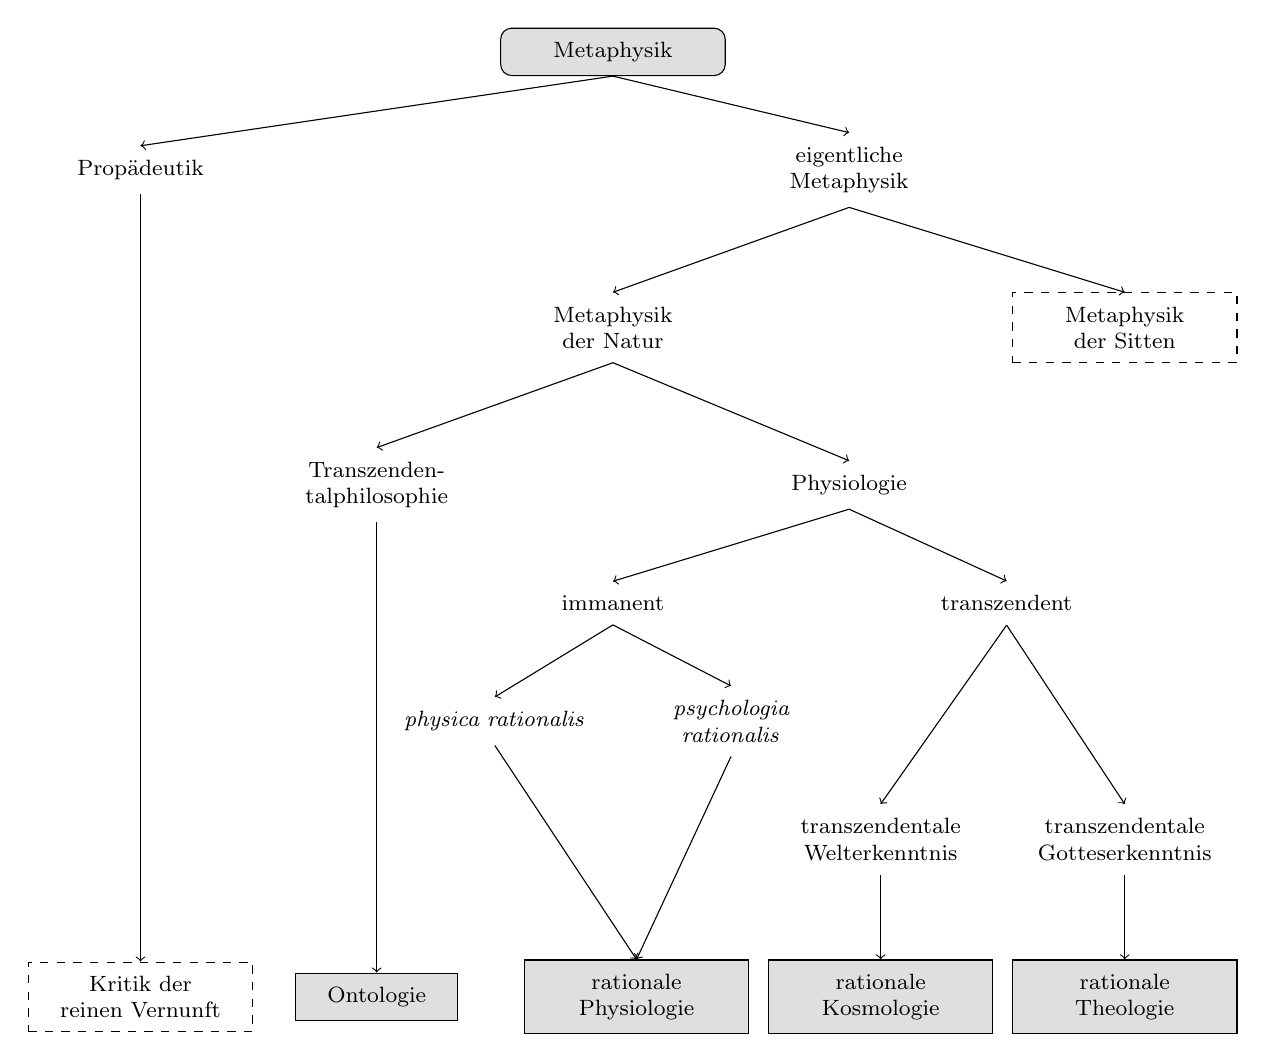
\begin{tikzpicture}[level distance=3cm,%
sibling distance=3cm,%
every node/.style={rectangle, thin, inner sep=0.5em,
minimum size=0.5em, align=center, text width=2.5cm, font=\footnotesize}]
\node (metaphysik) at (6cm,12cm) [fill=gray!25,draw, rounded corners]
{Metaphysik}; \node (prop) at (0cm,10.5cm) {Propädeutik};
\node (eigMet) at (9cm,10.5cm) {eigentliche Metaphysik};
\node (MdN) at (6,8.5) {Metaphysik der Natur};
\node (MdS) at (12.5,8.5) [draw,dashed] {Metaphysik der Sitten};
\node (TrP) at (3,6.5) {Transzen\-den\-tal\-phi\-lo\-so\-phie};
\node (Physio) at (9,6.5) {Physiologie};
\node (immanent) at (6,5) {immanent};
\node (transzendent) at (11,5) {transzendent};
\node (physica) at (4.5,3.5) {\emph{physica rationalis}};
\node (psycho) at (7.5,3.5) {\emph{psychologia rationalis}};
\node (Welt) at (9.4,2) {transzendentale Welterkenntnis};
\node (Gott) at (12.5,2) {transzendentale Gotteserkenntnis};
\node (KrV) at (0,0) [draw,dashed] {Kritik der reinen Vernunft};
\node (Ont) at (3,0) [fill=gray!25,draw, text width=1.7cm] {Ontologie};
\node (ratPh) at (6.3,0) [fill=gray!25,draw] {rationale Physiologie};
\node (ratKos) at (9.4,0) [fill=gray!25,draw] {rationale Kosmologie};
\node (ratTheo) at (12.5,0) [fill=gray!25,draw] {rationale Theologie};
% \node (metgen) at (3,-1.5) [text width=1.7cm,draw,dashed] {\emph{m.
% ge\-ne\-ra\-lis}}; \node (metspec) at (9.4,-1.5) [text width=8.7cm,draw,dashed]
% {\emph{metaphysica specalis}};
\draw[->] (metaphysik.south) -- (prop.north);
\draw[->] (metaphysik.south) -- (eigMet.north);
\draw[->] (eigMet.south) -- (MdN.north);
\draw[->] (eigMet.south) -- (MdS.north);
\draw[->] (MdN.south) -- (TrP.north);
\draw[->] (MdN.south) -- (Physio.north);
\draw[->] (Physio.south) -- (immanent.north);
\draw[->] (Physio.south) -- (transzendent.north);
\draw[->] (prop.south) -- (KrV.north);
\draw[->] (immanent.south) -- (physica.north);
\draw[->] (immanent.south) -- (psycho.north);
\draw[->] (transzendent.south) -- (Welt.north);
\draw[->] (transzendent.south) -- (Gott.north);
\draw[->] (TrP.south) -- (Ont.north);
\draw[->] (physica.south) -- (ratPh.north);
\draw[->] (psycho.south) -- (ratPh.north);
\draw[->] (Welt.south) -- (ratKos.north);
\draw[->] (Gott.south) -- (ratTheo.north);
\end{tikzpicture}


  \caption{Systematik des Metaphysikbegriffs nach
  \cite[][B~869--875]{Kant:KritikderreinenVernunft2003}, \cite[][III:
  543.27--547.15]{Kant:GesammelteWerke1900ff.}.}\label{abbildung:metaphysikeinteilung}
\end{minipage}
\end{figure}
Dabei unterscheidet er sogleich die \enquote{eigentliche Metaphysik} von der Vernunftkritik als deren
Propädeutik, wenngleich man letztere auch ohne weiteres zur Metaphysik
hinzurechnen könne. In einem engeren Sinn hingegen verstehe man unter Metaphysik
das System der reinen Erkenntnisse der Vernunft im \distanz{spekulativen}
Gebrauch, also unter Ausschluss der Metaphysik der Sitten (Tugendlehre und
Rechtsphilosophie). Die Metaphysik als Vernunfterkenntnis aus Begriffen -- wie
sie \name[Immanuel]{Kant} unter Bezug auf ihre Quellen bestimmt -- ist ohne
solche Einschränkungen offenkundig nicht deckungsgleich mit dem, was man für
gewöhnlich (und auch zu \name[Immanuel]{Kant}s Zeit) unter Metaphysik versteht.
Schließlich enthält sie insbesondere die gesamte Moral- und Rechtsphilosophie,
die \name[Immanuel]{Kant} unter dem Namen einer Metaphysik der Sitten
publiziert.
Diese wiederum ergibt damit einen Metaphysikbegriff, der nach den genannten
Einschränkungen, also der Eliminierung von Propädeutik und praktischer
Philosophie, koextensiv zu sein
scheint mit damals geläufigen Bestimmungen, wenn man ihn etwa mit der Einteilung
bei Christian \authorcite{Wolff:Psychologiaempirica1968}
vergleicht.\footnote{\label{anmerkung:wolffseinteilungdermetaphysik} Wobei
\authorcite{Wolff:Psychologiaempirica1968} die Psychologie und Theologie zunächst zu einer Pneumatologie
zusammenfasst.
\cite[Vgl.][\S~79]{Wolff:Discursuspraeliminarisdephilosophiaingenere1996}:
\enquote{Psychologia \&\ Theologia naturalis nonnunquam Pneumatic\ae\ nomine communi insigniuntur, \&\ Pneumatica
per spirituum scientiam definiri solet. Ontologia vero, Cosmolgia generalis \&\
Pneumatica communi Metaphysic\ae\ nomine compellantur. Est igitur Metaphysica
scientia entis, mundi in genere atque spirituum.} Dies entspricht der heute
geläufigen Aufteilung in eine \emph{metaphysica generalis} (Ontologie) und die drei
Teildisziplinen der \emph{metaphysica specialis} (Psychologie, Kosmologie, Theologie),
wobei sich eine solche Einteilung in allgemeine und spezielle Metaphysik weder
bei \authorcite{Wolff:Psychologiaempirica1968}, noch bei \name[Immanuel]{Kant} findet. Im Vergleich zu
\name[Immanuel]{Kant} fehlt bei \authorcite{Wolff:Psychologiaempirica1968} die rationale Physik, die
\name[Immanuel]{Kant} als Gegenstück zur rationalen Psychologie unter der Rubrik
\enquote{rationale Physiologie} neu einführt und dann in den
\titel{Metaphysischen Anfangsgründe der Naturwissenschaften} ausführlicher
behandelt. \mkbibparens{Dass die rationale Physiologie das Thema der
\titel{Metaphysischen Anfangsgründe} beschreibt, ergibt sich aus der Rolle, die
dem Begriff der Materie in der \titel{Kritik der reinen Vernunft} zugewiesen wird;
\cite[vgl.][B 875\,f.,]{Kant:KritikderreinenVernunft2003}
\cite[][III: 547.23--548.4]{Kant:GesammelteWerke1900ff.}}. Dafür schließt er
die empirische Psychologie aus der Metaphysik aus und räumt ihr nur noch unter
pragmatischen Gesichtspunkten einen Platz in der Philosophie ein
\mkbibparens{\cite[vgl.][B~876\,f.,]{Kant:KritikderreinenVernunft2003}
\cite[][III: 548.9--28]{Kant:GesammelteWerke1900ff.}}. Gerade in dem letzten
Punkt kommt zum Ausdruck, dass \name[Immanuel]{Kant} die Systematik nicht mehr wie
\authorcite{Wolff:Psychologiaempirica1968} inhaltlich -- anhand des Objekts --,
sondern methodisch -- nach Maßgabe der Erkenntnisquellen -- fundiert.}

Die Einteilung folgt dabei Überlegungen zur Art des Erwerbs einer Erkenntnis,
die -- wie in Kapitel \ref{subsection:Vernunfterkenntnis:MathematikPhilosophie}
gesehen -- deren Form ausmacht. Beispielsweise unterteilt er die immanente
Physiologie in Physik und Psychologie in Abhängigkeit davon, ob uns die
Gegenstände durch den äußeren oder den inneren Sinn gegeben
werden.\footnote{\cite[Vgl.][B 874]{Kant:KritikderreinenVernunft2003},
\cite[][III: 546.36--547.10]{Kant:GesammelteWerke1900ff.}.} Insofern ist
die inhaltliche Bestimmung des Metaphysikbegriffs sekundär und von der
methodischen Bestimmung, die sich an den Erkenntnisquellen orientiert, abhängig.
In der \titel{Kritik der Urteilskraft} heißt es entsprechend, dass \enquote{es
in der Einteilung einer Vernunftwissenschaft gänzlich auf diejenige
Verschiedenheit der Gegenstände ankommt, deren Erkenntnis verschiedener
Prinzipien bedarf}\footnote{\cite[][B xiii]{Kant:KritikderUrteilskraft2009},
\cite[][V: 172.17--19]{Kant:GesammelteWerke1900ff.}.}.
%
%
\item\label{InteresseDerMetaphysik} Bezüglich ihres \emph{Interesses} ist die
Metaphysik auf die Ideen Gott, Freiheit und Unsterblichkeit ausgerichtet, welche ihren eigentlichen und
einzigen Zweck ausmachen.\footnote{\enquote{Diese unvermeidlichen Aufgaben der
reinen Vernunft selbst, sind \ori{Gott, Freiheit} und \ori{Unsterblichkeit}. Die
Wissenschaft aber, deren Endabsicht mit allen ihren Zurüstungen eigentlich nur
auf die Auflösung derselben gerichtet ist, heißt \ori{Metaphysik}}
\mkbibparens{\cite[][B~7]{Kant:KritikderreinenVernunft2003}, \cite[][III:
31.6--9]{Kant:GesammelteWerke1900ff.}}. \enquote{Die Metaphysik hat zum
eigentlichen Zwecke ihrer Nachforschung nur drei Ideen: \ori{Gott, Freiheit} und
\ori{Unsterblichkeit} \punkt. Alles, womit sich diese Wissenschaft sonst
beschäftigt, dient ihr bloß zum Mittel, um zu diesen Ideen und ihrer Realität zu
gelangen} \mkbibparens{\cite[][B~395]{Kant:KritikderreinenVernunft2003},
\cite[][III: 260.20--24]{Kant:GesammelteWerke1900ff.}}.} Dabei nutzt
\name[Immanuel]{Kant} aus, dass die wichtigsten Fragen unserer Vernunft, welche auch wegen ihrer
Relevanz im Fokus der Aufklärung stehen (vornehmlich also die Religion), gerade
diejenigen Fragen sind, die (ausschließlich) aus reiner Vernunft heraus zu
behandeln sind.\footnote{\enquote{Und gerade in diesen letzteren Erkenntnissen,
welche über die Sinnenwelt hinausgehen, wo Erfahrung gar keinen Leitfaden, noch
Berichtigung geben kann, liegen die Nachforschungen unserer Vernunft, die wir,
der Wichtigkeit nach, für weit vorzüglicher, und ihre Endabsicht für viel
erhabener halten, als alles, was der Verstand im Felde der Erscheinungen lernen
kann, wobei wir, sogar auf die Gefahr zu irren, eher alles wagen, als daß wir
so angelegene Untersuchungen aus irgend einem Grunde der Bedenklichkeit, oder
aus Geringschätzung und Gleichgültigkeit aufgeben sollten}
\mkbibparens{\cite[][B~6\,f.,]{Kant:KritikderreinenVernunft2003} \cite[][III:
30.24--31.12]{Kant:GesammelteWerke1900ff.}}. Dies spricht auch gegen eine immer
wieder zu vernehmende Unterstellung, das traditionelle Interesse an
Erkenntnissen \emph{a priori} gründe in deren Immunität gegenüber Irrtümern
\parencite[siehe
z.\,B.][\pno~2\,f.]{Christensen:TestimonyMemoryandtheLimitsoftheaPriori1997}.}
Sie betreffen das \singlequote{Übersinnliche}, also diejenigen Gegenstände einer
Erkenntnis, die nicht auf der Grundlage von Erfahrung zu beantworten sind,
sondern verlangen, über den Bereich der Erfahrung hinaus zu gehen.
In den \titel{Fortschritten der Metaphysik} nennt \name[Immanuel]{Kant} die
Themenfelder, die das Interesse an der Metaphysik begründet, sogar als mögliches
\emph{Definiens} des Metaphysikbegriffs.\footnote{Siehe die retrospektive
Darstellung in \cite[][A
9\,f.,]{Kant:WelchessinddiewirklichenFortschrittediedieMetaphysikseitLeibnitzensundWolfsZeiteninDeutschlandgemachthat?1900ff.} \cite[][XX: 260.3--6]{Kant:GesammelteWerke1900ff.}: \enquote{Dieser Endzweck,
auf den die ganze Metaphysik angelegt ist, ist leicht zu entdecken, und kann in
dieser Rücksicht eine Definition derselben begründen: \enquote{sie ist die
Wissenschaft, von der Erkenntnis des Sinnlichen zu der des Übersinnlichen durch
die Vernunft fortzuschreiten.}}} Es sind dies die Themen, die -- so glaubt
\name[Immanuel]{Kant} -- in der Entwicklung des Metaphysikbegriffs stets prägend
blieben und welche die eigentliche Bestimmung der Philosophie -- ihren
Weltbegriff -- ausmachen.
\end{nummerierung}



Die quellenorientierte Definition dient dem Ziel, dem \emph{Schulbegriff} der
Philosophie gerecht zu werden, indem sie eine einheitliche und trennscharfe,
also den Richtlinien der Definitionslehre gemäße Bestimmung des Begriffs der
Metaphysik festlegt. Da Metaphysik den Kern der Philosophie, nämlich die
eigentliche Philosophie bildet, ist damit der Begriff der Philosophie ebenso
festgelegt. Die Berechtigung dieser Festlegung ergibt sich nun aus der Kongruenz
mit dem Weltbegriff der Philosophie, der sich an \enquote{der Beziehung aller
Erkenntnis auf die wesentlichen Zwecke der menschlichen
Vernunft ({teleologia rationis humanae})}\footnote{\cite[][B
867]{Kant:KritikderreinenVernunft2003}, \cite[][III: 542.27--28]{Kant:GesammelteWerke1900ff.}.} orientiert.
Wir könnten sagen, dass die grundlegende Definition derselben nach
ihren Quellen den \emph{Schulbegriff} der Metaphysik angibt, ihre Beziehung zu den
Themen Gott, Freiheit und Unsterblichkeit aber auf den \emph{Weltbegriff} derselben
verweist, \enquote{der dasjenige [enthält], was jedermann notwendig
interessiert}\footnote{\cite[][B~867]{Kant:KritikderreinenVernunft2003}, \cite[][III:
543.31--32]{Kant:GesammelteWerke1900ff.}.}, und was daher \enquote{doch als
Naturanlage (metaphysica naturalis)
wirklich}\footnote{\cite[][B~21]{Kant:KritikderreinenVernunft2003}, \cite[][III:
41.3]{Kant:GesammelteWerke1900ff.}.} ist.

Inhaltlich versucht \name[Immanuel]{Kant} Kontinuität zu wahren. Insofern die
Metaphysik im engere Sinne nur die Metaphysik der Natur umfasse, ergibt sich am
Ende der Einteilung die \singlequote{klassische} Aufteilung in Ontologie,
Physiologie (unter Einschluss der Psychologie), Kosmologie und Theologie.
Differenzen sind vor allem im Ausschluss aller empirischen Erkenntnisse
auszumachen und in den übergeordneten Einteilungen.
\authorcite{Wolff:Discursuspraeliminarisdephilosophiaingenere1996} fasst
beispielsweise Theologie und Psychologie zur Pneumatologie zusammen, weil sie
beide von \singlequote{Geistern} (\emph{spiritus})
handeln.\footcite[Vgl.][\S~79]{Wolff:Discursuspraeliminarisdephilosophiaingenere1996}
Da \name[Immanuel]{Kant} auf Einteilungen nach solchen rein inhaltlichen
Gesichtspunkten verzichtet, ergeben sich die Ähnlichkeiten erst auf der
untersten Ebene der Systematisierung.


Es ist von Bedeutung festzuhalten, dass der zentrale
Ausgangspunkt der Bestimmung des Metaphysikbegriffs der methodische ist, also
der Verweis auf die Quellen der Metaphysik aus reiner Vernunft. Damit ist
grundlegend, was vorhin im Zentrum der Überlegungen zu \name[Immanuel]{Kant}s
sozialer Erkenntnistheorie stand: Was wir aus reiner Vernunft erkennen können
-- also die Metaphysik --, das darf nicht im Modus bloß historischer Kenntnis
für wahr gehalten werden. Bis hierher könnte man versucht sein zu vermuten, wir
könnten nun einfach auf Metaphysik verzichten und damit die Forderung des
Selbstdenkens umgehen. Dass dieser Weg aber nicht gangbar ist, ergibt sich -- so
werden wir gleich sehen -- daraus, dass Metaphysik den Kern der Philosophie
ausmacht: \enquote{Und doch ist Metaphysik die eigentliche, wahre
Philosophie!}\footnote{\cite[][A 39]{Kant:ImmanuelKantsLogik1977}, \cite[][IX:
32.36--37]{Kant:GesammelteWerke1900ff.}.}  \name[Immanuel]{Kant} verwendet die
Termini Philosophie und Metaphysik (fast) gleichbedeutend -- genau genommen
identifiziert er die Metaphysik mit der \emph{reinen} Philosophie, der
Erkenntnis aus reiner Vernunft, die sich nicht auf empirische Prinzipien
stützt.\footnote{\cite[Vgl.][B~869]{Kant:KritikderreinenVernunft2003},
\cite[][III: 543.27--544.8]{Kant:GesammelteWerke1900ff.}. Siehe auch
\cite[][B~878]{Kant:KritikderreinenVernunft2003}, \cite[][III:
549.13--16]{Kant:GesammelteWerke1900ff.}: \enquote{Metaphysik also, sowohl der
Natur, als der Sitten, vornehmlich die Kritik der sich auf eigenen Flügeln
wagenden Vernunft, welche \ori{vorübend} (propädeutisch) vorhergeht, machen
eigentlich allein dasjenige aus, was wir im echten Verstande Philosophie nennen
können.}} Es ist diese reine Philosophie, deren Inhalte wir niemals auf die
Autorität anderer hin für wahr halten dürfen, wenn wir mündig und selbstbestimmt
denken wollen. Und dies erläutert dann auch, warum wir nach
\name[Immanuel]{Kant} eigentlich nicht Philosophie als System wahrer
Erkenntnisse, sondern ausschließlich die Tätigkeit des Philosophierens zu lernen
haben.

Ich rekurrierte oben auf den \emph{Weltbegriff der Philosophie}, um die
Akzentuierung bestimmter Erkenntnisbereiche innerhalb der
Aufklärungsprogrammatik zu beschreiben. Danach war sie die Wissenschaft von den
letzten Zwecken der Vernunft und als solche mit der Bestimmung des Menschen
befasst. Im Kapitel \ref{subsection:DieBestimmungdesMenschen} über die
Bestimmung des Menschen sahen wir, dass die Philosophie ihrem Weltbegriffe nach
im Fokus der Aufklärung steht, weil sie Inhalte thematisiert, die jeden Menschen
notwendig angehen. Auf der Grundlage der Kapitel
\ref{section:MuendigkeitundPhilosophie} lässt sich nun zeigen, dass
Philosophie ebenso ihrem Schulbegriff nach im Zentrum des \enquote{\emph{sapere
aude!}} steht, weil sie diesem Schulbegriffe nach der Inbegriff rationaler
Erkenntnisse ist. \enquote{Philosophie ist {\punkt} das System der
philosophischen Erkenntnisse oder der Vernunfterkenntnisse aus Begriffen. Das
ist der Schulbegriff von dieser Wissenschaft.}\footnote{\cite[][A
23]{Kant:ImmanuelKantsLogik1977}; \cite[][IX:
23.30--32]{Kant:GesammelteWerke1900ff.}.} Philosophische Erkenntnis ist nun aber
eine rationale Erkenntnis, die im Unterschied zu mathematischer Erkenntnis
diskursiv und nicht intuitiv ist; der Gesamtbereich rationaler Erkenntnis
zerfällt also in Mathematik und (\singlequote{reine}) Philosophie. Rationale
Erkenntnis ist diejenige Erkenntnis, der eine bloß historische Kenntnis nicht
angemessen ist (wobei Einschränkungen für die Mathematik
gelten\footnote{Siehe dazu Kapitel
\ref{subsubsection:EndlichesundUnendlichesErkennen}.}).
Also ist es gerade die Metaphysik und mit ihr die (\singlequote{reine})
Philosophie, bei der wir aufgefordert sind, uns in unseren Überzeugungen nicht
nach der Auskunft anderer zu richten, sondern unsere \emph{eigene} vernünftige
Einsicht zu suchen. Wie der Weltbegriff die
Philosophie aus inhaltlichen Gesichtspunkten heraus in das Zentrum der
Aufklärung stellte, so ist sie ihrem Schulbegriff nach formal im Fokus des \enquote{sapere aude}.

Zwischen Schul- und Weltbegriff der Philosophie besteht kein Widerstreit, so als
beschrieben sie verschiedene und miteinander unvereinbare, in Konkurrenz
zueinander oder auch nur unverbunden nebeneinander stehende Projekte.
Es ließe sich zwar \emph{prima facie} vermuten, dass der Weltbegriff beschreibt,
wie eine aufgeklärte Philosophie sein \emph{soll}, während der Schulbegriff den \emph{Status quo}
der damaligen akademisch betriebenen Philosophie beschreibt, die in ihrem Tun
die Absichten der Aufklärung verkennt, weil \enquote{sie nur als eine von den
Geschicklichkeiten zu gewissen beliebigen Zwecken angesehen
wird.}\footnote{\cite[][B 867]{Kant:KritikderreinenVernunft2003}; \cite[][III:
543.33--34]{Kant:GesammelteWerke1900ff.}. Siehe zu dieser Deutung z.\,B.
\cite[][481]{Doering:UeberKantsLehrevonBegriffundAufgabederPhilosophie1885}:
\enquote{Das ist also das Gesammtresultat [sic] dieser Untersuchung, daß uns
Kant vor die Alternative stellt, die Philosophie als Vernunftkünstler nach dem
Schulbegriffe als universelles System des Wissens, oder als weisheitsstrebende
nach dem Weltbegriffe als Inbegriff der allen Menschen angelegenen Erkenntnisse
zu betreiben.}} In der Tat aber gehen beide Hand in Hand, insofern der
Schulbegriff das zur Praxis notwendige Modell philosophischer Theorie beschreibt
(auf die Anbindung an die Praxis verweist der Begriff der
\singlequote{Welt}).\footnote{\cite[Vgl.][89]{Kleinhans:DerenquotePhilosophinderneuerenGeschichtederPhilosophie1999}.
\authorfullcite{Trawny:DasIdealdesWeisen2008} sieht im
Schulbegriff der Philosophie die (notwendigen, aber nicht hinreichenden) formalen Voraussetzungen
artikuliert, die eine Erkenntnis erfüllen muss, um als philosophisch zu
gelten \parencite[vgl.][467]{Trawny:DasIdealdesWeisen2008}. Siehe zum
Zusammenhang beider Begriffe auch die Arbeit von
\authorfullcite{Boehr:PhilosophiefuerdieWelt2003}, der den Weltbegriff mit der
Forderung nach Popularität, den Schulbegriff hingegen mit der Forderung nach
Gründlichkeit verbunden sieht, dabei aber einen engen Zusammenhang beider
Begriffe hervorhebt \parencite[vgl.][183--190]{Boehr:PhilosophiefuerdieWelt2003}.}
Wie in Kapitel \ref{chapter:AufklaerungundWissenschaft} dargestellt, verlangt
der Weltbegriff der Philosophie, demgemäß sie dasjenige Wissen vereint, dass wir
benötigen, um unserer Bestimmung als Menschen gerecht zu werden, in geringem
Umfang auch empirisches Wissen. Wir benötigen die \singlequote{Weltkenntnis} der
physischen Geographie und vor allem der pragmatischen Anthropologie. Aber dieses
Wissen ist doch ausgerichtet auf einen Kern, den uns nur die Metaphysik, und innerhalb der
Metaphysik speziell die Metaphysik der Sitten gewährt; schließlich ist die Moral
die Wissenschaft von der ganzen Bestimmung des Menschen.\footnote{Siehe Seite
\pageref{Anmerkung:GanzeBestimmung}.}


Der Schulbegriff bestimmt die Philosophie als System aller philosophischen
Erkenntnisse, also aller diskursiven\footnote{Zu dem Begriff der Diskursivität
siehe Kapitel \ref{subsubsection:BegriffderDiskursivitaet}.} Vernunfterkenntnisse, d.\,i.
der rationalen, aber nicht mathematischen, oder der \emph{metaphysischen} Erkenntnisse. Ihrem
Schulbegriffe nach ist die Philosophie daher im Kern Metaphysik: \enquote{das
System der reinen Vernunft (Wissenschaft), die ganze (wahre sowohl als scheinbare)
philosophische Erkenntnis aus reiner Vernunft im systematischen Zusammenhange
{\punkt} heißt
\ori{Metaphysik}}\footnote{\cite[][B 869]{Kant:KritikderreinenVernunft2003},
\cite[][III: 543.29--544.2]{Kant:GesammelteWerke1900ff.}. Siehe auch
\cite[][B 873]{Kant:KritikderreinenVernunft2003},
\cite[][III: 546.8--11]{Kant:GesammelteWerke1900ff.}:
\enquote{Alle reine Erkenntnis a priori macht also, vermöge des besondern
Erkenntnisvermögens, darin es allein seinen Sitz haben kann, eine besondere
Einheit aus, und Metaphysik ist diejenige Philosophie, welche jene Erkenntnis in
dieser systematischen Einheit darstellen soll.}}. \enquote{Metaphysik also
{\punkt} mach[t] eigentlich allein dasjenige aus, was wir im echten Verstande
Philosophie nennen können.}\footnote{\cite[][B
878]{Kant:KritikderreinenVernunft2003}, \cite[][III:
549.13--16]{Kant:GesammelteWerke1900ff.}.} Und es sind  die Themen und Urteile
der Metaphysik, die \name[Immanuel]{Kant} als philosophische Erkenntnisse
bezeichnet und von der die Aufklärungsforderung sagt, wir sollen sie nicht auf
die Autorität anderer hin übernehmen.

\subsection{Die Unverzichtbarkeit der
Metaphysik}\label{paragraph:DieUnverzichtbarkeitderMetaphysik}
Die Aufforderung, metaphysische Urteile nicht auf die Autorität anderer hin zu
übernehmen, impliziert für sich genommen noch nicht die Aufforderung, selbst
Metaphysik zu betreiben. Könnten wir annehmen, dass \name[Immanuel]{Kant} die
Ansicht vertritt, dass sich metaphysische Fragen gar nicht objektiv beantworten
lassen -- wie er es bezüglich der \emph{Noumena} zu behaupten scheint --, dann bliebe uns
auch die gänzliche Urteilsenthaltung. Dass wir anderen nicht glauben sollen, was
sie uns über Metaphysik sagen, heißt nicht, dass wir dies selbst erkennen
müssten. Wir glauben niemandem, der behauptet, uns die Lottozahlen vom nächsten
Samstag sagen zu können; aber deswegen denken wir nicht, wir müssten diese
selbst vorhersagen.

Die Frage, wie \name[Immanuel]{Kant} zur Möglichkeit von Metaphysik steht, ist
nicht leicht zu beantworten, wie aus den gegensätzlichen Angaben
\name[Immanuel]{Kant}s und insbesondere auch den unterschiedlichen
Interpretationen hervorgeht.\footnote{So spricht \authorcite{Walsh:KantandMetaphysics1976} recht
passend von einem \enquote{scandal to philosophy generally and to Kantian scholarship in
particular that commentators are unable to agree about \name[Immanuel]{Kant}'s
attitude to metaphysics} (\cite[][372]{Walsh:KantandMetaphysics1976}). Zur
Auseinandersetzung um die Frage, ob \name[Immanuel]{Kant} selbst Metaphysiker
war, siehe die Übersicht in
\cite{Funke:DieDiskussionumdiemetaphysischeKantinterpretation1976}.} So sei es
einerseits \enquote{demütigend für die menschliche Vernunft, daß sie in ihrem
reinen Gebrauche nichts ausrichtet, und sogar noch einer Disziplin bedarf, um
ihre Ausschweifungen zu bändigen, und die Blendwerke, die ihr daher kommen, zu
verhüten.}\footnote{\cite[][B 823]{Kant:KritikderreinenVernunft2003},
\cite[][III: 517.4--7]{Kant:GesammelteWerke1900ff.}.} Solche Äußerungen nähren
die Ansicht, \name[Immanuel]{Kant} sei der \distanz{Alleszermalmer der
Metaphysik}, wie \authorfullcite{Mendelssohn:MorgenstundenoderVorlesungenueberdasDaseynGottes1785} ihn in den
\titel{Morgenstunden}
nannte.\footnote{\cite[Vgl.][Vorbericht]{Mendelssohn:MorgenstundenoderVorlesungenueberdasDaseynGottes1785}.} Auf der anderen Seite beteuert \name[Immanuel]{Kant}, das \distanz{kritische
Geschäft} sei nur der Auftakt zum
doktrinalen\footnote{\cite[Vgl.][B x]{Kant:KritikderUrteilskraft2009},
\cite[][V: 170.20--22]{Kant:GesammelteWerke1900ff.}.}, und stellt eine
Metaphysik der Natur in Aussicht, die zumindest teilweise 1786 in Form der \titel{Metaphysischen
Anfangsgründen der Naturwissenschaft} das Licht der literarischen Welt erblickt.

Während \name[Immanuel]{Kant}s
Standpunkt zur Frage nach der \emph{Möglichkeit} eigentümlich dunkel bleibt --
man bedenke, dass dies gerade die Hauptfrage seines Hauptwerkes ist --, äußert
er sich sehr klar und unmissverständlich zur \emph{Notwendigkeit} von
Metaphysik. Das Pendant zum Weltbegriff und seiner Beziehung auf den
Endzweck der Vernunft -- die ganze Bestimmung des Menschen -- im Falle der
Philosophie ist dann im Falle der Metaphysik das \singlequote{Bedürfnis} der
Vernunft. Fraglich bleibt nur, ob Metaphysik damit eine Aufgabe unseres
Nachdenkens bleibt, die nicht endgültig aufzulösen ist oder von deren Auflösung
wir noch weit entfernt sind -- wie dies der Verweis auf das Ideal des
Philosophen und den Lehrer im Ideal der \titel{Kritik der reinen Vernunft}
suggeriert\footnote{\cite[Vgl.][B 866\,f.,]{Kant:KritikderreinenVernunft2003}
\cite[][III: 542.19-542.37]{Kant:GesammelteWerke1900ff.}.} --, oder ob
wenigstens ein Grundstein bereits gelegt ist. Auf diesen Punkt werde ich gleich
eingehen; doch bevor die Frage nach der Möglichkeit von Metaphysik diskutiert
wird, möchte ich zunächst fragen, inwiefern wir sie überhaupt \emph{benötigen}.


Bekanntlich bezeichnet \name[Immanuel]{Kant} die Metaphysik als
unvermeidlich, weil der menschlichen Vernunft ein \singlequote{Bedürfnis} nach
Metaphysik innewohne. Deswegen könne auch niemand auf die Beschäftigung mit
Metaphysik und das Fällen metaphysischer Urteile verzichten:
\begin{quote}
Es ist nämlich umsonst, \ori{Gleichgültigkeit} in Ansehung solcher
Nachforschungen erkünsteln zu wollen, deren Gegenstand der menschlichen Natur
\ori{nicht gleichgültig} sein kann. Auch fallen jene vorgeblichen
\ori{Indifferentisten},
so sehr sie sich auch durch die Veränderung der Schulsprache in einem populären Tone unkenntlich zu machen gedenken, wofern sie
nur überall etwas denken, in metaphysische Behauptungen unvermeidlich zurück,
gegen die sie doch so viel Verachtung
vorgaben.\footnote{\cite[][A~x]{Kant:KritikderreinenVernunft2003};
\cite[][IV: 8.28--34]{Kant:GesammelteWerke1900ff.}. Eine Parallelstelle findet
sich in der \titel{Logik}: \enquote{Was aber Metaphysik betrifft: so scheint
es, als wären wir bei Untersuchung metaphysischer Wahrheiten stutzig geworden.
Es zeigt sich jetzt eine Art von \ori{Indifferentism} gegen diese
Wissenschaft, da man es sich zur Ehre zu machen scheint, von metaphysischen
Nachforschungen, als von bloßen \ori{Grübeleien}, verächtlich zu reden.}
\mkbibparens{\cite[][A 39]{Kant:ImmanuelKantsLogik1977},
\cite[][IX: 32.31--36]{Kant:GesammelteWerke1900ff.}}}
\end{quote}
Der Indifferentist glaubt, es sei gar nicht nötig, in metaphysischen Fragen ein
objektiv gültiges Urteil abzugeben.\footnote{Hier ist nicht der Ort, sich
ausführlich mit dem Begriff des Indifferentismus auseinander zu setzen, den
\name[Immanuel]{Kant} den theologischen Auseinandersetzungen des 17. und 18.
Jahrhunderts entnimmt. Siehe dazu die kurze Einordnung sowie die weiteren
Verweise in \cite[][\pno~511\,f.,]{Gierl:PietismusundAufklaerung1997} sowie
\cite[][\pno~513\,f.]{Albrecht:Eklektik1994}. \name[Immanuel]{Kant} übersetzt
den Ausdruck \enquote{Indifferentism} durchgängig mit
\enquote{Gleichgültigkeit} \mkbibparens{siehe
\cite[][A 96]{Kant:BeobachtungenueberdasGefuehldesSchoenenundErhabenen1977},
\cite[][II: 250.11]{Kant:GesammelteWerke1900ff.}} und bezeichnet die
Indifferentisten in Fragen der Moral auch als \emph{Latitudinarier
der Neutralität} \mkbibparens{\cite[][B
9]{Kant:DieReligioninnerhalbderGrenzenderblossenVernunft1977}, \cite[][VI:
22.19--28]{Kant:GesammelteWerke1900ff.}}.} Diese Gleichgültigkeit gegenüber
metaphysischen Fragen sei -- so \name[Immanuel]{Kant} -- eine \enquote{Wirkung
{\punkt} der gereiften \ori{Urteilskraft} des Zeitalters,}\footnote{\cite[][A
xi]{Kant:KritikderreinenVernunft2003}, \cite[][IV:
9.2--3]{Kant:GesammelteWerke1900ff.}.} welches auch \enquote{das eigentliche
Zeitalter der \ori{Kritik}}\footnote{\cite[][A
xi]{Kant:KritikderreinenVernunft2003}, \cite[][IV:
9.33]{Kant:GesammelteWerke1900ff.}.} sei und \emph{als solches}
von \name[Immanuel]{Kant} wohl auch noch immer als das Zeitalter der Aufklärung
angesehen wird. Doch eine solche Gleichgültigkeit lasse sich nur scheinbar
aufrecht erhalten, denn Metaphysik -- oder Philosophie im eigentlichen Sinne --
sei nicht verzichtbar, sie lasse sich höchstens mehr oder minder gut unkenntlich
machen. \name[Immanuel]{Kant} nennt -- so ergibt sich bei genauerem Lesen --
zwei Gründe für die Unmöglichkeit eines Verzichts auf Metaphysik, die ich im
folgenden explizieren werde:
Zum einen gebe es innerhalb der Metaphysik Aufgaben, die wir nicht vermeiden können
(Abschnitt
\ref{subsubsection:UnvermeidlicheAufgabenderMetaphysik}), zum
zweiten liege die Metaphysik jedem Denken als solchem zugrunde
(Abschnitt \ref{subsubsection:MetaphysikalsGrundlageunseresDenkens}).\footnote{Diese Punkte
entsprechen der Einteilung der Metaphysik in eine \emph{metaphysica generalis}
und eine \emph{metaphysica specialis}. Ich gehe an dieser Stelle nicht weiter
auf diese Einteilung  und ihre historischen Hintergründe ein. Siehe dazu ausführlich
\cite{Vollrath:DieGliederungderMetaphysikineineMetaphysicaGeneralisundeineMetaphysicaSpecialis1962}.}

\begin{nummerierung}
\item\label{subsubsection:UnvermeidlicheAufgabenderMetaphysik}
Als ersten Grund für die Unmöglichkeit, auf Metaphysik einfach zu verzichten,
führt \name[Immanuel]{Kant} an, es gebe Themen und Fragestellungen, mit denen
wir uns früher oder später beschäftigen müssen, weil sie der menschlichen
Natur nicht gleichgültig sein \emph{können}:
\begin{quote}
Diese unvermeidlichen Aufgaben der reinen Vernunft selbst, sind \ori{Gott},
\ori{Freiheit} und \ori{Unsterblichkeit}. Die Wissenschaft aber, deren
Endabsicht mit allen ihren Zurüstungen eigentlich nur auf die Auflösung
derselben gerichtet ist, heißt \ori{Metaphysik}, deren Verfahren im Anfange
\ori{dogmatisch} ist, d.\,i. ohne vorhergehende Prüfung des Vermögens oder
Unvermögens der Vernunft zu einer so großen Unternehmung zuversichtlich die
Ausführung übernimmt.\footnote{\cite[][B 7]{Kant:KritikderreinenVernunft2003},
\cite[][III: 31.6--12]{Kant:GesammelteWerke1900ff.}.}
\end{quote}
Warum sind diese Aufgaben unvermeidlich? Können wir nicht sehr gut auskommen,
ohne die Frage nach der Existenz Gottes zu stellen? Müssen wir diese Frage
beantworten oder können wir uns nicht einfach auf den Standpunkt eines
generellen \emph{Ignorabimus} zurückziehen? Gerade wenn die Vernunftkritik
zeigt, dass genannte Fragen die Grenzen unseres Wissens übersteigen, wenn sie
\enquote{das Wissen aufheb[t], um zum Glauben Platz zu
bekommen,}\footnote{\cite[][B xxx]{Kant:KritikderreinenVernunft2003},
\cite[][III: 19.6]{Kant:GesammelteWerke1900ff.}.} scheint doch Metaphysik als
\emph{Erkenntnis} des Übersinnlichen obsolet zu werden.
Die Frage beispielsweise, ob das Universum einen Anfang in der Zeit hat, oder ob
es räumlich in Grenzen eingeschlossen oder unendlich (oder unbegrenzt, aber
endlich) ist, können wir unbeantwortet lassen. Wir können genauso eine Antwort
verweigern wie in vertrauten Fällen, wenn wir nach einer Auskunft gefragt werden
und eine Antwort unter Verweis auf unser eigenes Nichtwissen verweigern. In
vielen Fällen ist möglich, was die antiken Skeptiker als
{\epoche} bezeichnen.

Es ist verlockend, \name[Immanuel]{Kant}s Festhalten an der Notwendigkeit dieser
Fragen einfach der Tatsache zuzuschreiben, dass er im 18. Jahrhundert lebte und
die Selbstverständlichkeiten dieser Zeit artikulierte. Aber diese
Selbstverständlichkeiten müssen nicht die unseren sein. In Kapitel
\ref{chapter:AufklaerungundWissenschaft} war die Situation ähnlich:
\name[Immanuel]{Kant} stellt in der Aufklärungsschrift ganz selbstverständlich
die Religion in das Zentrum seiner Ausführungen, weil Unmündigkeit in Fragen der
Religion die schädlichste und entehrendste sei. Warum dies so ist, erörtert er
nicht; und der Leser mag den Verdacht hegen, dass dieses Urteil den
zeitlichen Umständen des 18. Jahrhunderts geschuldet ist. Es fand sich jedoch eine
Rechtfertigung dieses Urteils in den Überlegungen zur Bestimmung des Menschen,
die sich an der Ethik orientiert und Fragen unserer Handlungsausrichtung
betrifft.\footnote{Siehe oben, Kap. \ref{subsection:DieBestimmungdesMenschen}.}
Und dies scheint mir auch im Falle der Metaphysik der Hintergrund von
\name[Immanuel]{Kant}s Urteil zu sein, es gebe ein Bedürfnis der Vernunft. Unter
einem \singlequote{Bedürfnis} darf freilich kein empirisches Bedürfnis
verstanden werden, welches wir \singlequote{empfinden} und das uns dazu drängt,
diese Fragen zu stellen. Wenn das Bedürfnis ein Bedürfnis \emph{der Vernunft}
ist, dann kann es nicht bloß subjektiv unbefriedigend, sondern dann muss es
objektiv unvernünftig sein, diese Fragen nicht zu stellen.

Urteilsenthaltung ist überall dort keine vernünftige
Option, wo eine Frage gestellt wird, auf die eine Antwort zu haben für unser
Handeln nötig ist. \name[Immanuel]{Kant} denkt, dass die Fragen nach Gott und
Unsterblichkeit der Seele eben solche Fragen sind, die wir nicht übergehen
können, weil wir sie bei der vernünftigen Orientierung unseres Handelns
beantworten \emph{müssen}. Er wird diese Fragen in den Bereich des
\enquote{moralischen Glaubens} verweisen und behaupten, wir könnten sie wegen
eines Bedürfnisses der Vernunft, die Bedingungen unseres moralischen
Handlungserfolgs als gegeben anzunehmen, nicht abweisen. Entsprechend schreibt
\name[Immanuel]{Kant}:
\begin{quote}
Man kann aber das Bedürfnis der Vernunft als zwiefach ansehen: \ori{erstlich} in
ihrem \ori{theoretischen}, \ori{zweitens} in ihrem \ori{praktischen} Gebrauch.
Das erste habe ich eben angeführt; aber man sieht wohl, daß es nur bedingt sei,
d.\,i. wir müssen die Existenz Gottes annehmen, wenn wir über die ersten
Ursachen alles Zufälligen, vornehmlich in der Ordnung der wirklich in der Welt
gelegten Zwecke, \ori{urteilen wollen}.  Weit wichtiger ist das Bedürfnis der
Vernunft in ihrem praktischen Gebrauche, weil es unbedingt ist, und wir die
Existenz Gottes voraus zu setzen nicht bloß alsdann genötigt werden, wenn wir
urteilen \ori{wollen}, sondern weil wir \ori{urteilen
müssen}.\footnote{\cite[][A 315]{Kant:Washeisst:SichimDenkenorientieren?1977},
\cite[][VIII: 139.6--15]{Kant:GesammelteWerke1900ff.}.}
\end{quote}
Wir können Fragen der theoretischen Vernunft unbeantwortet lassen und unser
Urteil zurückhalten. Aber Fragen der praktischen Vernunft lassen keine
{\epoche} zu, weil wir \emph{handeln müssen} und dazu \emph{urteilen
müssen}.

Nun ist es zunächst die Metaphysik \emph{der Sitten}, also Metaphysik im
praktischen Vernunftgebrauch, die wir aus diesem Grund nicht vermeiden können.
Wir können nicht handeln, ohne uns irgendwie zu Fragen der Moral zu verhalten.
Und moralische Aussagen, die nicht davon handeln, wie wir \emph{de facto}
handeln, sondern davon, wie wir handeln \emph{sollen}, können nicht durch die
Erfahrung beantwortet werden, sind also allesamt metaphysisch. Dass
\name[Immanuel]{Kant} sie im genannten Zitat nicht erwähnt, ist sicherlich der
Tatsache geschuldet, dass er sich in der \titel{Kritik der reinen Vernunft} eben
ausschließlich mit dem reinen spekulativen Vernunftgebrauch, also der Metaphysik
der Natur befasst. Im praktischen Vernunftgebrauch wiederum scheint
\name[Immanuel]{Kant} die Möglichkeit objektiver Urteile für nicht weiter
problematisch zu halten.

Nach \name[Immanuel]{Kant} gibt es darüber hinaus im spekulativen
Vernunftgebrauch metaphysische Urteile, die durch keine objektiv gültigen Gründe
entschieden werden können, die aber mit unseren Handlungen so eng verbunden
sind, dass uns eine Antwort abverlangt wird: Dazu gehören die Existenz Gottes
und die Unsterblichkeit unserer Seele, sowie unsere Freiheit im Sinne einer
Unabhängigkeit von uns determinierenden Ursachen.\footnote{\enquote{Diese
Postulate sind die der \ori{Unsterblichkeit}, der \ori{Freiheit}, positiv
betrachtet (als der Kausalität eines Wesens, so fern es zur intelligibelen Welt
gehört), und das \ori{Dasein Gottes}. Das \ori{erste} fließt aus der praktisch
notwendigen Bedingung der Angemessenheit der Dauer zur Vollständigkeit der
Erfüllung des moralischen Gesetzes; das \ori{zweite} aus der notwendigen
Voraussetzung der Unabhängigkeit von der Sinnenwelt und des Vermögens der
Bestimmung seines Willens, nach dem Gesetze einer intelligibelen Welt, d.\,i.
der Freiheit; das \ori{dritte} aus der Notwendigkeit der Bedingung zu einer
solchen intelligibelen Welt, um das höchste Gut zu sein, durch die Voraussetzung
des höchsten selbständigen Guts, d.\,i. des Daseins Gottes}
\mkbibparens{\cite[][A 238\,f.,]{Kant:KritikderpraktischenVernunft1974}
\cite[][V: 132.19--29]{Kant:GesammelteWerke1900ff.}}.}
\name[Immanuel]{Kant} sagt, dass die Unsterblichkeit der Seele und die Existenz
Gottes jenseits des Bereichs unseres Wissens liegen, wir aber begründeter und
vernünftiger Weise an sie \singlequote{glauben} können.\footnote{Bezüglich
unserer Freiheit sagt er freilich, dass wir wenigstens ihr \emph{Möglichkeit}
wissen können: \enquote{Freiheit ist aber auch die einzige unter allen Ideen
der spek. Vernunft, wovon wir die Möglichkeit a priori \emph{wissen}, ohne sie
doch einzusehen, weil sie die Bedingung des moralischen Gesetzes ist, welches
wir wissen} \mkbibparens{\cite[][A 5]{Kant:KritikderpraktischenVernunft1974},
\cite[][V: 4.7--10]{Kant:GesammelteWerke1900ff.}}.} Diese Fragen, bei denen
unsere Erkenntnis an ihre Grenzen stößt, betreffen ausgerechnet das
\emph{Interesse} der Metaphysik und korrespondieren dem Weltbegriff der
Philosophie.

\item\label{subsubsection:MetaphysikalsGrundlageunseresDenkens}
Der andere Grund lautet: Jeder stellt metaphysische Behauptungen auf, sobald
\enquote{er nur überall etwas
denk[t]}\footnote{\cite[][A x]{Kant:KritikderreinenVernunft2003}, \cite[][IV:
8.33]{Kant:GesammelteWerke1900ff.}.}. Die transzendentale Analytik zeigt, dass
jeder objektive Gedanke ein metaphysisches Fundament hat: Es gibt keinen
Gedanken, der frei von Metaphysik ist, weil jedes Denken von Kategorien und
Grundsätzen des reinen Verstandes Gebrauch macht. Der \textit{Verstand} schreibt
der Natur \emph{a priori} theoretische Gesetze vor, die Kategorien und Grundsätze der
transzendentalen Analytik. Hier fügt sich die \singlequote{kopernikanische
Wende}\footnote{Der Ausdruck \enquote{kopernikanische Wende} oder
\enquote{kopernikanische Revolution} lässt sich bei \name[Immanuel]{Kant}
selbst nicht belegen und auch der genaue Sinn der Analogie ist umstritten
\parencite[siehe
dazu][]{Schoenecker:Kantskopernikanisch-newtonischeAnalogie2011}.} oder -- im
originalen Wortlaut \name[Immanuel]{Kant}s -- die \enquote{Revolution der
Denkart}\footnote{\cite[][B xi]{Kant:KritikderreinenVernunft2003}, \cite[][III:
9.19]{Kant:GesammelteWerke1900ff.}.}, die in der Vorrede zur zweiten Auflage der
Vernunftkritik beschrieben wird, in die Aufklärungskonzeption ein:
Es ist denkbar, dass der Verstand autonom ist, wir uns also in der Erkenntnis
der natürlichen Welt als frei handelnd und nicht als passiv erleidend verstehen
können, weil angenommen werden kann, dass sich die Dinge in der
Welt als Gegenstände unserer Erkenntnis nach unserem Verstand und seinen
Gesetzen richten.\footnote{\cite[Vgl.][B
xvi--xviii]{Kant:KritikderreinenVernunft2003}, \cite[][III:
12.3--33]{Kant:GesammelteWerke1900ff.}.} Die Notwendigkeit metaphysischer
Grundlagen des Denkens führt uns zum Begriff der Autonomie des Denkens und
Erkennens. Dieser Begriff wurde bereits im
\ref{section:KantalsliberalerAufklaerer}. Kapitel verwendet und vorausgesetzt,
aber noch nicht geklärt. Hier ergibt sich gleich die Gelegenheit, den Begriff autonomen
Erkennens mit Inhalt zu füllen.
\end{nummerierung}

\Revision{Man mag hier einwenden: Im Anhang zur transzendentalen Dialektik
findet sich ein weiterer Ansatz einer \distanz{kritischen Metaphysik}, die sich von einer dogmatischen
Metaphysik primär darin unterscheidet, dass ihre Erkenntnisse als
\emph{regulativ} verstanden werden. \name[Immanuel]{Kant} rekurriert dort
zunächst auf die Ansicht, dass es ein natürlicher Hang \emph{der Vernunft} (und
nicht etwa individueller Irrtum) sei, dass wir uns über die Grenzen der Vernunft
hinaus bewegen.\footnote{\cite[Vgl.][B 670]{Kant:KritikderreinenVernunft2003},
\cite{Kant:GesammelteWerke1900ff.}.} Es ist kein Irrtum, sondern Ausdruck von
Vernunft, sich um immer größere Systematik und Einheitlichkeit unseres Wissens
zu bemühen. Und die größte Einheitlichkeit sei erst durch Abschluss der
Wissenschaft im Bereich der Metaphysik möglich. Dies sei auch nicht schädlich,
wenn man nur im Auge behalte, dass damit nichts objektiv über die Gegenstände
der Metaphysik erwiesen
ist.\footnote{\cite[Vgl.][B 673--675]{Kant:KritikderreinenVernunft2003},
\cite[][III: 428.19--430.2]{Kant:GesammelteWerke1900ff.}.}}

\Revision{Diese Überlegungen überführt \name[Immanuel]{Kant} in der
\titel{Kritik der Urteilskraft} in die Idee einer formalen Zweckmäßigkeit der Natur für unsere
Urteilskraft. Ich werde dies unter dem Titel der \enquote{Heautonomie}
diskutieren\footnote{Siehe unten, ab S. \pageref{AutonomiederUrteilskraft}.}.
Nach Auskunft der \titel{Prolegomena} gehören diese Überlegungen als
\singlequote{Scholien} gar nicht in das System der Metaphysik und gingen auch
nur diejenigen etwas an, die professionell Metaphysik betreiben und um
Vollständigkeit bemügt
sind.\footnote{\cite[Vgl.][\S~60]{Kant:ProlegomenazueinerjedenkuenftigenMetaphysikdiealsWissenschaftwirdauftretenkoennen1977},
\cite[][IV: 362.5--365.4]{Kant:GesammelteWerke1900ff.}.} In der \titel{Kritik
der Urteilskraft} wird die Frage nach der größtmöglichen Systematik und
Einheitlichkeit schließlich nicht mehr als Aufgabe der Vernunft beschrieben,
sondern der reflektierenden Urteilskraft zugeschrieben und unter dem Stichwort
der \enquote{Heautonomie} oder der \enquote{formalen Zweckmäßigkeit der Natur}
behandelt. Ich werde dieser (späteren) Einordnung folgen und die
\singlequote{regulative Metaphysik} der \titel{Kritik der reinen Vernunft} hier
nicht weiter behandeln.}

Bevor ich auf die Autonomie des Denkens eingehe, fasse ich kurz zusammen:
Es gibt zwei Gründe, aus denen wir nicht auf Metaphysik verzichten können; und
diesen Gründen korrespondieren jeweils eigene Bereiche der Metaphysik: Wir
müssen metaphysische Behauptungen machen, sobald wir \emph{handeln} wollen. Und wir müssen andere
metaphysische Behauptungen machen, wenn wir \emph{denken} wollen. Zu den
Voraussetzungen des Handelns gehören die Metaphysik der Sitten, die rationale
Psychologie und die rationale Theologie. Zur Voraussetzung des Denkens gehört
die Ontologie.

\subsection{Autonomie und Spontaneität}\label{subsection:MetaphysikundAutonomie}
Nach \name[Immanuel]{Kant}s Bestimmung dessen, was es heißt, selbst zu denken,
sollen wir unsere je eigene Vernunft zum obersten Probierstein der Wahrheit
machen. Diese Forderung erwies sich jedoch \emph{prima facie} als zu
anspruchsvoll, wenn wir daraus die Aufforderung ableiten, die Wahrheit einer
jeden Überzeugung selbst -- ohne Vertrauen auf die Mitteilungen anderer oder gar
ohne Rekurs auf die eigene Wahrnehmung -- zu kontrollieren. In Kapitel
\ref{section:MuendigkeitundPhilosophie} zeigte ich, dass dieser Anspruch nur auf
rationale Erkenntnisse, also Mathematik und Philosophie bezogen werden kann. Im
folgenden werde ich zeigen, dass die Beziehung dieser Forderung auf die
Metaphysik als den Kern der Philosophie geeignet ist, die Aussage zu
interpretieren, wir sollten unsere eigene Vernunft zum obersten Probierstein der
Wahrheit machen.

Es sind die oberen Erkenntnisvermögen, die auf
Prinzipien a priori beruhen\footnote{\cite[Vgl.][B 243]{Kant:KritikderUrteilskraft2009}, \cite[][V:
345.5--6]{Kant:GesammelteWerke1900ff.}.} und daher a priori gesetzgebend und
somit \emph{autonom} sind. Obere Erkenntnisvermögen sind der Verstand, die
Vernunft und die Urteilskraft, wobei das Gesamt des oberen Erkenntnisvermögens
wahlweise als Vernunft oder als Verstand bezeichnet wird. Denn neben der
\singlequote{engeren} Verwendung als Ausdruck für eines der drei oberen
Erkenntnisvermögen neben \enquote{Urteilskraft} und \enquote{Vernunft} könne der
Ausdruck \enquote{Verstand} auch für das gesamte obere Erkenntnisvermögen
einschließlich Vernunft und Urteilskraft stehen.\footnote{\cite[Vgl.][BA
115\,f.,]{Kant:AnthropologieinpragmatischerHinsicht1977} \cite[][VII:
196.17--197.3]{Kant:GesammelteWerke1900ff.}.} Und manchmal verwendet
\name[Immanuel]{Kant} eben auch den Terminus \enquote{Vernunft} in einem weiten
Sinne als Ausdruck für das gesamt obere
Erkenntnisvermögen.\footnote{\cite[Vgl.][B 863]{Kant:KritikderreinenVernunft2003}, \cite[][III:
540.28]{Kant:GesammelteWerke1900ff.}.}

\phantomsection\label{Abschnitt:IstSinnlichkeiteinErkenntnisvermögen} Das untere
Erkenntnisvermögen hingegen ist nach \name[Immanuel]{Kant} das Vermögen sinnlicher Erkenntnisse.
Hier ließe sich aber fragen: Handelt es sich bei der Sinnlichkeit überhaupt um
ein Vermögen? In der Anthropologie findet sich ein Satz, der dies verneint:
\enquote{In Ansehung des Zustandes der Vorstellungen ist mein Gemüt entweder
\ori{handelnd} und zeigt \ori{Vermögen} (facultas), oder es ist \ori{leidend} und besteht in \ori{Empfänglichkeit}
(receptivitas).}\footnote{\cite[][BA
25]{Kant:AnthropologieinpragmatischerHinsicht1977},
\cite[][VII: 140.16--18]{Kant:GesammelteWerke1900ff.}.} Demnach ist der Verstand
als das gesamte obere Erkenntnisvermögen ein Vermögen, aber die Sinnlichkeit als bloße
Rezeptivität ist kein Vermögen; denn der Begriff des Vermögens setzt die
Fähigkeit zu einer Handlung -- zu einem aktiven Tun -- voraus, während die
Sinnlichkeit in einem bloß passiven Erleiden besteht. Später bezeichnet Kant die
Sinnlichkeit jedoch explizit als unteres Erkenntnisvermögen:
\begin{quote}
\ori{Verstand}, als das Vermögen zu \ori{denken} (durch \ori{Begriffe} sich
etwas vorzustellen), wird auch das \ori{obere} Erkenntnisvermögen (zum
Unterschiede von der Sinnlichkeit, als des \ori{unteren}) genannt, darum, weil
das Vermögen der Anschauungen (reiner oder empirischer) nur das Einzelne in
Gegenständen, dagegen das der Begriffe das Allgemeine der Vorstellungen
derselben, die \ori{Regel}, enthält, der das Mannigfaltige der sinnlichen
Anschauungen untergeordnet werden muß, um Einheit zur Erkenntnis des Objekts
hervorzubringen.\footnote{\cite[][BA
115]{Kant:AnthropologieinpragmatischerHinsicht1977},
\cite[][VII: 196.17--24]{Kant:GesammelteWerke1900ff.}.}
\end{quote}
In der \titel{Anthropologie} stellt Kant zunächst fest, dass Erkenntnis nur aus
dem \emph{Zusammenspiel} von Rezeptivität und Spontaneität resultieren kann. Die
Möglichkeit, Erkenntnis zu haben, die aus diesem Zusammenspiel beider Stämme
oder Grundquellen resultiert -- und nicht die Stämme selbst --, heiße nun
Erkenntnisvermögen.\footnote{\enquote{Ein \ori{Erkenntnis} enthält beides verbunden in sich und die Möglichkeit, eine solche zu haben, führt den Namen
des \ori{Erkenntnisvermögens} von dem vornehmsten Teil derselben, nämlich der
Tätigkeit des Gemüts, Vorstellungen zu verbinden, oder voneinander zu sondern}
\mkbibparens{\cite[][BA 25]{Kant:AnthropologieinpragmatischerHinsicht1977},
\cite[][VII: 140.18--22]{Kant:GesammelteWerke1900ff.}}.} Danach ist weder die
Sinnlichkeit noch der Verstand als Erkenntnisvermögen zu bezeichnen, sondern die Vermögen, die wir
vermittels des Zusammenspiels von Sinnlichkeit und Verstand besitzen. 

Nach \name[Immanuel]{Kant} gehören alle diejenigen Vorstellungen zum unteren
oder sinnlichen Erkenntnisvermögen, bei denen sich das Gemüt (auch!) leidend
verhält. Zum oberen oder intellektuellen Erkenntnisvermögen gehören hingegen
diejenigen Vorstellungen, in Ansehung derer sich das Gemüt \emph{ausschließlich} tätig verhält, die also nur ein Tun
(das Denken) enthalten:
\begin{quote}
Vorstellungen, in Ansehung deren sich das Gemüt leidend verhält, durch welche
also das Subjekt \ori{affiziert} wird (dieses mag sich nun selbst affizieren
oder von einem Objekt affiziert werden), gehören zum \ori{sinnlichen}:
diejenigen aber, welche ein bloßes \ori{Tun} (das  Denken) enthalten, zum
\ori{intellektuellen} Erkenntnisvermögen. Jenes wird auch das \ori{untere},
dieses aber das \ori{obere} Erkenntnisvermögen
genannt.\footnote{\cite[][BA 25]{Kant:AnthropologieinpragmatischerHinsicht1977},
\cite[][VII: 140.23--28]{Kant:GesammelteWerke1900ff.}. Nach
\authorfullcite{Brandt:KritischerKommentarzuKantsenquoteAnthropologieinpragmatischerHinsicht1999}
handelt es sich dabei um eine distanzierte Darstellung fremder Redegebräuche,
denen sich \name[Immanuel]{Kant} nicht selbst anschließe, sie sogar zurückweise
\parencite[vgl.][174]{Brandt:KritischerKommentarzuKantsenquoteAnthropologieinpragmatischerHinsicht1999}.
Leider nennt
\authorcite{Brandt:KritischerKommentarzuKantsenquoteAnthropologieinpragmatischerHinsicht1999}
keine Gründe für diese These, die mit dem Wortlaut des Textes so gar nicht
harmonieren möchte.}
\end{quote}
Es gibt kein Erkenntnisvermögen, das ausschließlich sinnlich oder rezeptiv wäre;
in diesem Falle wäre es eben nicht einmal ein Vermögen. Nach dieser Einteilung
gehören lediglich die \emph{reinen} Verstandesbegriffe (und Grundsätze) zum
oberen Erkenntnisvermögen, während alle empirischen Er\-kennt\-nis\-se -- also
alle empirischen Begriffe und Urteile -- zum unteren Erkenntnisvermögen zu
zählen sind, wenngleich es natürlich dennoch Erkenntnisse sind, die der
\emph{Verstand} hervorbringt. Sinnlichkeit (Rezeptivität) ist selbst kein
Erkenntnisvermögen, weil sie selbst nicht urteilt und daher keine Erkenntnisse
hervorbringt. Nur der Verstand urteilt, aber er urteilt zum einen über das, was
er sinnlich wahrnimmt, und zum anderen über das, wofür er keiner Wahrnehmung
bedarf.

Es scheint mir notwendig zu sein zu sagen, dass wir in unterschiedlichen
Bedeutungen von Sinnlichkeit und Verstand sprechen, je nachdem, ob wir sie als
Erkenntnisstämme (oder -quellen) oder als Erkenntnisvermögen betrachten. Die
beiden Stämme der Erkenntnis sind jeweils für sich genommen nicht in der Lage,
Erkenntnisse zu produzieren. Als Erkenntnisvermögen genommen handelt es sich
nicht um die jeweiligen Erkenntnisstämme in Reinform, sondern um das Vermögen
(also die Fähigkeit), Erkenntnisse zu generieren, die als rationale Erkenntnisse
(\emph{a priori} und \emph{ex principiis}) dem oberen Erkenntnisvermögen
(\singlequote{Verstand}) oder als empirische Erkenntnisse (\emph{a posteriori}
und \emph{ex datis}) dem unteren Erkenntnisvermögen (\singlequote{Sinnlichkeit}) angehören.

Soll der Zusammenhang mit dem Begriff der Autonomie betont werden, dann bietet
sich der Ausdruck \enquote{Vernunft} an: \enquote{Nun nennt man das Vermögen,
nach der Autonomie, d.\,i. frei (Prinzipien des Denkens überhaupt gemäß) zu
urteilen, die Vernunft.}\footnote{\cite[][A 25]{Kant:DerStreitderFakultaeten1977},
\cite[][VII: 27.30--32]{Kant:GesammelteWerke1900ff.}.} Hier ist die Vernunft als
das obere Erkenntnisvermögen angesprochen und als solches mit dem Begriff der
Autonomie verbunden. Es ist nicht nur die Vernunft im engeren Sinne, sondern die
oberen Erkenntnisvermögen als solche, denen Autonomie zukommt. Autonomie
ist die Eigenschaft des Subjekts, nach \enquote{Prinzipien des Denkens
überhaupt} zu urteilen, und ein Vermögen, welches über eigene Prinzipien
\emph{a priori} verfügt, ist ein oberes
Erkenntnisvermögen.\footnote{\enquote{Daß es drei Arten der Antinomie gibt, hat
seinen Grund darin, daß es drei Erkenntnisvermögen: Verstand, Urteilskraft und
Vernunft gibt, deren jedes (als oberes Erkenntnisvermögen) seine Prinzipien a
priori haben muß} \mkbibparens{\cite[][B 243]{Kant:KritikderUrteilskraft2009},
\cite[][V: 345.3--6]{Kant:GesammelteWerke1900ff.}}.} Die oberen
Erkenntnisvermögen sind daher der Ort, an dem sich \name[Immanuel]{Kant}s
Aufklärungsprogramm entfaltet.

Prinzipien \emph{a priori} und die aus ihnen gewonnenen Erkenntnisse nennt
\name[Immanuel]{Kant} philosophisch und das System
philosophischer Erkenntnisse Metaphysik. Autonom sein heißt entsprechend, über
ein metaphysisches Fundament zu verfügen, wie es bei den oberen
Erkenntnisvermögen der Fall ist. Da es drei obere Erkenntnisvermögen gibt --
Verstand, Vernunft und Urteilskraft --, finden wir auch drei Fälle von Autonomie
vor\footnote{\cite[Vgl.][32]{Kant:ErsteEinleitungindieenquoteKritikderUrteilskraft2009},
\cite[][XX: 225.21--32]{Kant:GesammelteWerke1900ff.}.}: Die \textit{Vernunft}
gibt der \emph{Freiheit} das Gesetz, den kategorischen Imperativ.
Der \emph{Verstand} gibt der \emph{Natur} das Gesetz, die Kategorien und
Grundsätze des reinen Verstandes.\footnote{\enquote{Der Verstand ist a priori
gesetzgebend für die Natur als Objekt der Sinne, zu einem theoretischen
Erkenntnis derselben in einer möglichen Erfahrung. Die Vernunft ist a priori
gesetzgebend für die Freiheit und ihre eigene Kausalität, als das Übersinnliche
in dem Subjekte, zu einem unbedingt-praktischen Erkenntnis}
\mkbibparens{\cite[][B liii]{Kant:KritikderUrteilskraft2009},
\cite[][V: 195.4--8]{Kant:GesammelteWerke1900ff.}}.
Siehe auch \cite[][B xi--xiii]{Kant:KritikderUrteilskraft2009}, \cite[][V:
171.4--172.22]{Kant:GesammelteWerke1900ff.}.} Und die \emph{Urteilskraft} gibt
\emph{sich selbst} ein Gesetz (das transzendentale Prinzip der formalen
Zweckmäßigkeit der Natur), weswegen sie nicht einfach als \emph{autonom},
sondern genauer als \emph{heautonom} bezeichnet werden
könnte.\footnote{\enquote{Die Gesetzgebung
durch Naturbegriffe geschieht durch den Verstand und ist theoretisch. Die Gesetzgebung
durch den Freiheitsbegriff geschieht von der Vernunft und ist bloß praktisch}
\mkbibparens{\cite[][B xvii]{Kant:KritikderUrteilskraft2009},
\cite[][V: 174.32--34]{Kant:GesammelteWerke1900ff.}}. \enquote{Die Urteilskraft hat also auch ein Prinzip a priori
für die Möglichkeit der Natur, aber nur in subjektiver Rücksicht, in sich, wodurch die nicht der Natur (als Autonomie),
sondern ihr selbst (als Heautonomie) für die Reflexion über jene ein Gesetz
vorschreibt, welches man das Gesetz der Spezifikation der Natur in Ansehung
ihrer empirischen Gesetze nennen könnte} \mkbibparens{\cite[][B
xxxvii]{Kant:KritikderUrteilskraft2009}, \cite[][V:
185.35--186.3]{Kant:GesammelteWerke1900ff.}}.
\enquote{Diese Gesetzgebung müßte man eigentlich Heautonomie nennen, da die
Urtheilskraft nicht der Natur, noch der Freyheit, sondern lediglich ihr selbst
das Gesetz giebt und kein Vermögen ist, Begriffe von Objekten hervorzubringen,
sondern nur mit denen, die ihr anderweitig gegeben sind, vorkommende Fälle zu
vergleichen und die subjective Bedingungen der Möglichkeit dieser Verbindung a
priori anzugeben}
\mkbibparens{\cite[][32]{Kant:ErsteEinleitungindieenquoteKritikderUrteilskraft2009},
\cite[][XX: 225.27--32]{Kant:GesammelteWerke1900ff.}}.}


Dass ein Erkenntnisvermögen autonom ist, heißt gerade, dass es auf Prinzipien
\emph{a priori} beruht. Und in Anlehnung an \name[Immanuel]{Kant}s Begriff der
Metaphysik ergibt sich: Ein
Erkenntnisvermögen ist autonom genau dann, wenn es eine Grundlage in der
Metaphysik hat. Das ist eine begriffliche Wahrheit über den Begriff der
Autonomie. Diese Autonomie ist eine \emph{Folge} davon, dass es sich um
obere Erkenntnisvermögen handelt; um den Ursprung der Autonomie zu erkennen,
gilt es somit, den Begriff des oberen Erkenntnisvermögens zu explizieren. In der
\titel{Kritik der reinen Vernunft} klärt \name[Immanuel]{Kant} den Begriff eines
oberen Erkenntnisvermögens nicht explizit, gibt aber folgende Auskunft, die
zunächst dafür spricht, den Begriff des oberen Erkenntnisvermögens unter
Rückgriff auf den Begriff der Autonomie zu erläutern:
\enquote{Ich verstehe hier aber unter Vernunft das ganze obere
Erkenntnisvermögen, und setze also das Rationale dem Empirischen
entgegen.}\footnote{\cite[][B 863]{Kant:KritikderreinenVernunft2003},
\cite[][III: 540.27--29]{Kant:GesammelteWerke1900ff.}.}
Das Wort \enquote{also} zeigt an, dass die Identifizierung der Vernunft mit dem
Rationalen eine Folge dessen ist, dass sie als das ganze obere
Erkenntnisvermögen betrachtet wird. Das obere Erkenntnisvermögen ist also ein
Vermögen rationaler Erkenntnis und wird als solches dem Vermögen, empirische
Erkenntnis zu generieren, gegenübergestellt. Danach ist ein oberes
Erkenntnisvermögen ein solches, mittels dessen wir zu rationalen Erkenntnissen,
also Erkenntnissen \emph{ex principiis} fähig sind. Das untere
Erkenntnisvermögen, zu dem Sinnlichkeit und Einbildungskraft gehören, liefert
empirische Erkenntnisse oder Erkenntnisse \emph{ex datis}.\footnote{Siehe hierzu
oben Kapitel \ref{section:MuendigkeitundPhilosophie}.}

In der \titel{Anthropologie in pragmatischer Hinsicht} findet sich eine
Bestimmung des Begriffs des oberen Erkenntnisvermögen, die auf ein anderes
Merkmal als den Erwerb rationaler Erkenntnisse verweist. Hier steht nicht der
Begriff der Vernunft, sondern der Begriff des \emph{Verstandes} im Vordergrund:
\begin{quote}
In Ansehung des Zustandes der Vorstellungen ist mein Gemüt entweder
\ori{handelnd} und zeigt \ori{Vermögen} (facultas), oder es ist \ori{leidend}
und besteht in \ori{Empfänglichkeit} (receptivitas). {\punkt} Vorstellungen, in
Ansehung deren sich das Gemüt leidend verhält {\punkt} gehören zum
\ori{sinnlichen}: diejenigen aber, welche ein bloßes \ori{Tun} (das Denken)
enthalten, zum \ori{intellektuellen} Erkenntnisvermögen. Jenes wird auch das
\ori{untere}, dieses aber das \ori{obere} Erkenntnisvermögen
genannt.\footnote{\cite[][BA 25]{Kant:AnthropologieinpragmatischerHinsicht1977},
\cite[][VII: 140.16--28]{Kant:GesammelteWerke1900ff.}.}
\end{quote}
Der Verstand ist das Vermögen der Spontaneität im Unterschied zur Sinnlichkeit
als der Rezeptivität: \enquote{Wollen wir die \ori{Rezeptivität} unseres Gemüts,
Vorstellungen zu empfangen, so fern es auf irgend eine Weise affiziert wird,
\ori{Sinnlichkeit} nennen; so ist dagegen das Vermögen, Vorstellungen selbst
hervorzubringen, oder die \ori{Spontaneität} des Erkenntnisses, der
\ori{Verstand}.}\footnote{\cite[][B 75]{Kant:KritikderreinenVernunft2003},
\cite[][III: 75.5--8]{Kant:GesammelteWerke1900ff.}. Siehe auch Kapitel
\ref{subsection:DiskursiverVerstandundsinnlicheAnschauung} dieser Arbeit.}. Im
Unterschied zu den bisher betrachteten Explikationen geht es \name[Immanuel]{Kant} hier
\emph{expressis verbis} um eine Bestimmung des Begriffs des oberen
Erkenntnisvermögens; das angeführte Merkmal ist also grundlegend und nicht --
wie das der Autonomie -- abgeleitet. Dieses grundlegende Merkmal des oberen
Erkenntnisvermögens ist die Selbsttätigkeit oder \emph{Spontaneität}, die den
Verstand als den einen Stamm der menschlichen Erkenntnis neben der Sinnlichkeit
ausmacht. Zu sagen, dass ein solches Vermögen \emph{als} oberes
Erkenntnisvermögen ein Vermögen ist, das über Prinzipien \emph{a priori}
verfügt, heißt, den Begriff der Selbsttätigkeit oder Spontaneität weiter zu
explizieren.

In Kapitel \ref{subsection:DerBegriffdesSelbstdenkens} hatte ich von einem
positiven und einem negativen Begriff des Selbstdenkens in Analogie zum
negativen und positiven Begriff der Freiheit in der \titel{Grundlegung zur
Metaphysik der Sitten} gesprochen. Hier begegnet ein solcher Kontrast wiederum.
Als Verstand ist das obere Erkenntnisvermögen nicht leidend äußeren Einflüssen
unterworfen, sondern selbsttätig -- spontan. Dies entspricht dem negativen
Begriff des Selbstdenkens. Als Vernunft wiederum verfügt das obere
Erkenntnisvermögen über eigene Grundsätze \emph{a priori}; dies entspricht dem
positiven Begriff des Selbstdenkens. Diese Grundsätze, die autonomen Gesetze des
Verstandes und der Urteilskraft sowie der Vernunft sind der letzte Probierstein
der Wahrheit, den \name[Immanuel]{Kant} in seiner Konkretisierung des Begriffs
des Selbstdenkens anführt. Dieser Maßstab reicht freilich nicht aus, um an ihm
allein die Wahrheit unserer Urteile zu überprüfen.
Urteile können diesem Maßstab entsprechen und dennoch falsch sein. Aber ein
Urteil, welches diesen Maßstäben schon nicht entspricht, dessen Wahrheit ist
unmöglich und darf von uns auch nicht angenommen werden. Ich werde im folgenden
die Autonomie der Vernunft (\ref{AutonomiederVernunft}), des Verstandes
(\ref{AutonomiedesVerstandes}) und der Urteilskraft
(\ref{AutonomiederUrteilskraft}) beschreiben, um diesen Gedanken zu
konkretisieren.
\begin{nummerierung}
\item\label{AutonomiederVernunft} Die Vernunft gibt der
Freiheit das Gesetz. Wie \name[Immanuel]{Kant} insbesondere in der
\titel{Grundlegung zur Metaphysik der Sitten} betont, ist nur die Vorstellung von Autonomie in der Lage, den
allgemein bindenden Charakter moralischer Normen verständlich zu
machen.\footnote{\enquote{Es ist kein Wunder, wenn wir auf alle bisherige
Bemühungen, die jemals unternommen worden, um das Prinzip der Sittlichkeit
ausfündig zu machen, zurücksehen, warum sie insgesamt haben fehlschlagen müssen.
Man sahe den Menschen durch seine Pflicht an Gesetze gebunden, man ließe es sich
aber nicht einfallen, daß er nur seiner eigenen und dennoch allgemeinen
Gesetzgebung unterworfen sei, und daß er nur verbunden sei, seinem eigenen, dem
Naturzwecke nach aber allgemein gesetzgebenden, Willen gemäß zu handeln}
\mkbibparens{\cite[][BA 73]{Kant:GrundlegungzurMetaphysikderSitten1965},
\cite{Kant:GesammelteWerke1900ff.}}.}  Alle anderen, auf Heteronomie gegründeten
ethischen Theorien konnten den Begriff der Pflicht, der wir als endliche Wesen
unterworfen sind, nicht entwickeln. Und nur der Begriff der Autonomie mache es
möglich, dass ein Wesen als endliches Wesen Gesetzen unterworfen ist, die es
\emph{nötigen} und ihm \emph{befehlen}, und dennoch seine Würde (als
selbst gesetzgebend) bewahrt.\footnote{\Revision[Selbst]{\cite[Vgl.][BA 86\,f.]{Kant:GrundlegungzurMetaphysikderSitten1965},
\cite[][IV: 440.7--13]{Kant:GesammelteWerke1900ff.}.}} Dies mag zunächst paradox anmuten,
denn Grundsätze, die ich mir lediglich selbst gebe, scheinen doch solche zu
sein, von denen ich mich auch jederzeit selbst entbinden kann.\footnote{Vgl.
\cite[][226]{Pinkard:GermanPhilosophy1760-18602002}.} Deshalb dürfen wir
Autonomie nicht in einer Weise vorstellen, nach der wir uns die
bestimmenden Grundsätze selbst in einem willkürlichen Akt selbst geben. Es sind
Grundsätze, die uns als Vernunftwesen
ausmachen.\footnote{\cite[Vgl.][90-130]{Korsgaard:TheSourcesofNormativity1996},
hier speziell S.~90\,f. } Nach \authorcite{Roedl:Selbstgesetzgebung2011} ist das Gesetz identisch mit dem
Willen, weil es lediglich ausdrückt, dass der Wille praktische Vernunft
ist.\footnote{\cite[Vgl.][]{Roedl:Selbstgesetzgebung2011}. Sie dazu auch
\cite[][]{Menke:AutonomieundBefreiung2010}.} Sollte eine solche Interpretation
korrekt sein, dann wäre klar, wie dieser Begriff der Autonomie die Vereinbarkeit
von Freiheit und Vernunft gewährleistet: Frei sein hieße, in seinem Denken und
Handeln die Grundsätze zur Geltung zu bringen, die uns als Vernunftwesen
ausmachen.\footnote{Der Begriff der Autonomie als Vermögen der Vernunft, der Freiheit Gesetze
vorzuschreiben, wird in unzähligen Beiträgen zur \name[Immanuel]{Kant}forschung
besprochen. Diese Beiträge können an dieser Stelle weder referiert werden, noch
soll ihnen ein weiterer Beitrag an die Seite gestellt werden. Neben den bereits
genannten Beiträgen sind zu nennen:
\cite{Sturma:KantsEthikderAutonomie2004,Gunkel:SpontaneitaetundmoralischeAutonomie1989,
Shell:KantandtheLimitsofAutonomy2009,Shell:KantandtheenquoteParadoxofAutonomy2012}..}

Da theoretische und praktische Vernunft keine getrennten Vermögen sind, sondern
unterschiedliche Gebrauchsarten desselben Vermögens, liegt es nahe, dass die
Vernunft im engeren Sinne nicht nur in der Ethik und allgemein im Handeln als
praktische, sondern gerade im Erkennen als theoretische Vernunft wirksam
ist.\footnote{Dies behauptet auch
\authorfullcite{Larmore:TheAutonomyofMorality2008}, der sich dazu auf die
Beschreibung der kopernikanischen Wende in der Vorrede zur zweiten Auflage der
\titel{Kritik der reinen Vernunft} beruft
\parencite[vgl.][41]{Larmore:TheAutonomyofMorality2008}.} Von der Vernunft ist
nun aber sowohl ein realer als auch ein bloß formaler Gebrauch denkbar. Der
Gebrauch eines Erkenntnisvermögens heißt dabei \emph{real}, wenn es selbst
Begriffe und Grundsätze hervorbringt. Er heißt logisch oder \emph{formal}, wenn
das Erkenntnisvermögen lediglich auf bereits gegebene Begriffe und Erkenntnisse
angewandt wird.\footnote{\enquote{Es gibt von ihr [der Vernunft; A.\,G.], wie
von dem Verstande, einen bloß formalen, d.\,i. logischen Gebrauch, da die
Vernunft von allem Inhalte der Erkenntnis abstrahiert, aber auch einen realen,
da sie selbst den Ursprung gewisser Begriffe und Grundsätze enthält, die sie
weder von den Sinnen, noch vom Verstande entlehnt} \mkbibparens{\cite[][B
355]{Kant:KritikderreinenVernunft2003}, \cite[][III:
237.26--30]{Kant:GesammelteWerke1900ff.}}. Siehe auch
\cite[][\S~5]{Kant:Demundisensibilisatqueintelligibilisformaetprincipiis1968},
\cite[][II: 393.16--22]{Kant:GesammelteWerke1900ff.}.} In Ansehung der
Naturerkenntnis können wir von unserer Vernunft (als theoretische Vernunft)
jedoch nur einen {formalen}, keinen {realen} Gebrauch machen:
\begin{quote}
Die Gesetzgebung durch Naturbegriffe geschieht durch den Verstand und ist
theoretisch. Die Gesetzgebung durch den Freiheitsbegriff geschieht von der
Vernunft und ist bloß praktisch. Nur allein im Praktischen kann die Vernunft
gesetzgebend sein; in Ansehung des theoretischen Erkenntnisses (der Natur) kann
sie nur (als gesetzkundig vermittelst des Verstandes) aus gegebenen Gesetzen
durch Schlüsse Folgerungen ziehen, die doch immer nur bei der Natur
stehenbleiben.\footnote{\cite[][B xvii]{Kant:KritikderUrteilskraft2009},
\cite[][V: 174.32--175.2]{Kant:GesammelteWerke1900ff.}.}
\end{quote}
Dies ist damit gemeint, dass die Vernunft der Freiheit, nicht der Natur das
Gesetz gebe. Der formale oder logische Gebrauch der Vernunft liegt unserem
Denken in allen Bereichen zugrunde; aber nur in Bezug auf unser Handeln gibt sie
uns genuine Vernunftbegriffe (den \emph{Freiheitsbegriff}) und
Vernunftprinzipien (moralisch-praktische Gesetze, den \emph{kategorischen
Imperativ}) an die Hand. Deswegen ist die Vernunft nur in der
Moralphilosophie autonom, während in der Naturphilosophie der Verstand Autonomie
ausübt.

\begin{comment}
Nicht nur in Bezug auf unser äußeres Handeln, sondern gerade auch
in Bezug auf unser Denken ist von einem Sollen zu sprechen. Im Gegensatz zu
\authorcite{Wolff:Discursuspraeliminarisdephilosophiaingenere1996}, der die
empirische Psychologie als eine der Grundlagendisziplinen der Logik ansieht,
führt \name[Immanuel]{Kant} hier eine klare Trennung ein:
\begin{quote}
Einige Logiker setzen zwar in der Logik \ori{psychologische} Prinzipien voraus.
Dergleichen Prinzipien aber in die Logik zu bringen, ist ebenso ungereimt, als
Moral vom Leben herzunehmen. Nähmen wir die Prinzipien aus der Psychologie,
d.\,h. aus den Beobachtungen über unsern Verstand, so würden wir bloß sehen,
\ori{wie} das Denken vor sich geht und \ori{wie es ist} unter den mancherlei
subjektiven Hindernissen und Bedingungen; dieses würde also zur Erkenntnis bloß
\ori{zufälliger} Gesetze führen. In der Logik ist aber die Frage nicht nach
\ori{zufälligen}, sondern nach \ori{notwendigen} Regeln; -- nicht, wie wir
denken, sondern, wie wir denken
sollen.\footnote{\cite[][A 6]{Kant:ImmanuelKantsLogik1977},
\cite[][IX: 14.3--12]{Kant:GesammelteWerke1900ff.}.}
\end{quote}



\name[Immanuel]{Kant} glaubt, dass der Begriff der Autonomie das Rätsel lösen
könne, wie Gesetze präskriptive Kraft haben können, ohne sich auf einen
vorausgesetzten Zweck zu beziehen. Nun wird häufig genug bestritten, dass dieser
Argumentationsweg überzeugt. 

\authorfullcite{Larmore:TheAutonomyofMorality2008} schließt daraus gar, dass es
sich bei der Vernunft um ein \emph{rezeptives} Vermögen -- also nach
\name[Immanuel]{Kant} um \emph{Sinnlichkeit} -- handelt.\footnote{\enquote{[W]e
must conclude, in a very un-\name[Immanuel]{Kant}ian spirit, that reason at
bottom is a receptive faculty} \parencite[][44]{Larmore:TheAutonomyofMorality2008}.} Aber das ist
zunächst einfach aporetisch, denn es lässt die Frage offen, woher die Maßstäbe
der Vernunft überhaupt kommen sollen, wenn nicht aus der Vernunft selbst. Die
Vernunft ist ihr einziger Maßstab, weil es nichts anderes gibt noch geben kann, was ihr rechtmäßiger
Weise etwas vorschreiben kann. Die Vermutung, wir müssten darauf schauen, wie
Menschen \emph{de facto} denken, scheint ebenso absurd wie der Verweis auf
Introspektion. Wir wissen einfach nicht, woher wir Regeln der Vernunft
\emph{rezeptiv} nehmen sollten, was es heißt, den Gebrauch unserer Vernunft an
etwas anderem als ihr selbst zu messen.\footnote{Allerdings gibt es im Anschluss
an Überlegungen von \authorfullcite{Frege:LogischeUntersuchungen1993} eine Diskussion, ob Gesetze der Logik nicht einfach allgemeinere Gesetze sind.
\authorfullcite{Glueer:BedeutungzwischenNormundNaturgesetz2000} greift die
These, unser Denken sei wesentlich in normativen Vorgaben der Vernunft fundiert,
unter explizitem Verweis auf die in der \jaeschelogik{} vertretene Position an.
Wir sollten die Gesetze der Logik nicht als kategorische Vorschriften an die
Vernunft, die diese sich selbst gibt, ansehen, sondern als \singlequote{Gesetze
des Wahrseins} im Sinne \authorcite{Frege:LogischeUntersuchungen1993}s analog zu
Naturgesetzen: Logische Gesetze handeln von den allgemeinsten Zusammenhängen der
Welt. Und unter der Bedingung, dass wir Wahres denken wollen, sollten wir im Einklang
mit diesen Gesetzen denken
\parencite[vgl.][]{Glueer:BedeutungzwischenNormundNaturgesetz2000}. Dies
schließt offenkundig an Überlegungen
\authorfullcite{Quine:TwoDogmasofEmpiricism1951}s an, wonach es keine strikte
Trennung von apriorischen und aposteriorischen Erkenntnissen gibt, sondern nur
mehr oder minder zentrale und periphere Erkenntnisse
\parencite[vgl.][]{Quine:TwoDogmasofEmpiricism1951}. Siehe dagegen:
\cite{Roedl:NormundNatur2003}.}

Die Kritikpunkte setzen jedoch ein Autonomieverständnis voraus, das nicht
dasjenige \name[Immanuel]{Kant}s ist, insofern Autonomie und Vernunft als
getrennt betrachtet
werden.\footnote{\cite[Vgl.][75--77]{ONeill:ConstructionsofReason1989}.} Eine
eindeutige Folge ist, dass wir uns von einem legislatorischen
Autonomieverständnis distanzieren
müssen.\footnote{\authorfullcite{Menke:AutonomieundBefreiung2010} sieht den
Bruch mit diesem Autonomieverständnis in \name[Immanuel]{Kant}s Redeweise von
der \singlequote{\emph{eigenen} Gesetzgebung} (statt der
\singlequote{\emph{Selbst}gesetzgebung}) darüber hinaus auch sprachlich
vollzogen \parencite[vgl.][677]{Menke:AutonomieundBefreiung2010}.} Wenn
Autonomie heißt, dass wir nur an solche Gesetze gebunden sind, die wir uns
selbst \emph{gegeben} haben, dann treffen die genannten Einwände zu. Stattdessen
müssen wir Autonomie in der Richtung interpretieren, die
\authorfullcite{Korsgaard:TheSourcesofNormativity1996} vorgegeben hat: Es geht
nicht um Gesetze, die wir uns nach Belieben \emph{geben}, sondern um
die Gesetze, in denen wir unsere Identität
ausdrücken\footnote{\enquote{[T]he principle or law by which you determine your
actions is one that you regard as being expressive of \ori{yourself}. To
identify with such a principle or way of choosing is to be, in St Paul's famous
phrase, a law to yourself}
\parencite[][100]{Korsgaard:TheSourcesofNormativity1996}.} -- oder, um mit
\authorfullcite{Menke:AutonomieundBefreiung2010} zu sprechen: um ein Gesetz,
welches ein Subjekt \emph{ist}.\footnote{\enquote{Das Gesetz, in dessen Gehorsam
ich frei bin, ist nicht das Gesetz, das ich mir selbst gegeben habe, sondern das
ich mir selbst \ori{bin}} \parencite[][678]{Menke:AutonomieundBefreiung2010}.}
Der Autonomiebegriff \name[Immanuel]{Kant}s ist nicht \emph{legislatorisch}.\footnote{Siehe
\cite[][677--679]{Menke:AutonomieundBefreiung2010}, sowie die dort zitierte
Literatur.} Ob er \emph{expressivistisch} ist, mag hier dahingestellt sein. Aus
\name[Immanuel]{Kant}s Auskünften lässt sich eines leicht entnehmen: Unsere
Vernunft ist nicht autonom, weil wir die obersten Prinzipien selbst geben,
sondern weil wir sie \emph{a priori} erkennen. Die Prinzipien sind metaphysische
Erkenntnisse, die objektiv rational sind, von denen wir subjektiv aber
rationale oder historische Erkenntnis haben können.
\end{comment}
%
%
%
\item\label{AutonomiedesVerstandes} Der Verstand schreibt der Natur sein Gesetz
vor. Durch diesen Gedanken einer Autonomie des theoretischen Erkennens erläutert
\name[Immanuel]{Kant} die Möglichkeit einer Metaphysik der Natur: Der Ausgangspunkt der Verwirrung, mit
der die \titel{Kritik der reinen Vernunft} sich auseinandersetzt, lautet: Wie kann es
sein, dass wir durch bloßes Denken, ohne auf Erfahrung zurückzugreifen, etwas
darüber erkennen können, wie die Dinge, die unabhängig von uns existieren, sind?
In anderen Worten lässt sich fragen:
Wie ist Metaphysik (der Natur) möglich? Nicht verwunderlich ist es nach
\name[Immanuel]{Kant}, dass wir mit bloßer Vernunft etwas über unsere Vernunft
selbst ausmachen können. Deswegen kommt die Verwunderung, die ihn bei der Kritik
der reinen \emph{spekulativen} Vernunft antreibt, in \emph{dieser} Form nicht im
Kontext einer Kritik der reinen \emph{praktischen} Vernunft vor. Es wäre
naheliegend davon auszugehen, dass Erkenntnisse darüber, wie die Dinge in der Welt
unabhängig von uns sind, nur durch die Aktualisierung \emph{rezeptiver}
Fähigkeiten zu erlangen sind. In der zeitlichen Reihenfolge ist nach
\name[Immanuel]{Kant} auch klar, dass wir unser rezeptives Erkenntnisvermögen
aktualisieren müssen, ehe wir Wissen über die Welt erlangen können. Von diesem
Gedanken geht er in der \titel{Kritik der reinen Vernunft} aus, ohne ihn eigens
zu begründen. Dennoch dürfe man davon, dass der menschliche Verstand gleichsam
als \emph{tabula rasa} beginne, nicht darauf schließen, dass unsere
Erfahrungserkenntnis rein rezeptiv gewonnen werden könne. Vielmehr beinhalte sie
rationale Erkenntnis:
\begin{quote}
 Wenn aber gleich alle unsere Erkenntnis mit der Erfahrung anhebt, so entspringt
sie darum doch nicht eben alle aus der Erfahrung. Denn es könnte wohl sein, daß
selbst unsere Erfahrungserkenntnis ein Zusammengesetztes aus dem sei, was wir
durch Eindrücke empfangen, und dem, was unser eigenes Erkenntnisvermögen (durch
sinnliche Eindrücke bloß veranlaßt,) aus sich selbst hergibt, welchen Zusatz wir
von jenem Grundstoffe nicht eher unterscheiden, als bis lange Übung uns darauf
aufmerksam und zur Absonderung desselben geschickt gemacht
hat.\footnote{\cite[][B 1\,f.,]{Kant:KritikderreinenVernunft2003} \cite[][III:
27.14--21]{Kant:GesammelteWerke1900ff.}.}
\end{quote}
Sollte Metaphysik (der Natur) jedoch tatsächlich
möglich sein, dann muss einsichtig gemacht werden, wie ein Vermögen der
\emph{Spontaneität} die Welt so soll abbilden können, wie sie \emph{de facto
ist} (und nicht wie sie sein \emph{sollte}).

Die scheinbare Aporie, die mit der Frage nach der Möglichkeit metaphysischer
Naturerkenntnis einhergeht, hat die Form eines Dilemmas:
Unser Denken soll wahre Sätze generieren, die sich auf Gegenstände beziehen,
diese bestimmen und damit Sinn und Bedeutung
haben.\footnote{\cite[Vgl.][B 299]{Kant:KritikderreinenVernunft2003},
\cite[][III: 204.37--205.3]{Kant:GesammelteWerke1900ff.}. Bedeutung ist
\enquote{Beziehung aufs Objekt} \mkbibparens{\cite[][B 300]{Kant:KritikderreinenVernunft2003},
\cite[][III: 205.20--21]{Kant:GesammelteWerke1900ff.}}.} Nur wenn es eine
Beziehung zwischen unseren Vorstellungen und Dingen in der Welt gibt, verfügen
wir über Erkenntnisse.\footnote{Dies geht aus dem Begriff der Erkenntnis hervor.
Erkenntnis in einem \singlequote{eigentlichen} Sinn von objektiv gültigen
Urteilen (siehe dazu Anmerkung \ref{Anmerkung:ErkenntnisInZweierleiSinn} auf
Seite \pageref{Anmerkung:ErkenntnisInZweierleiSinn}) besteht in der
\enquote{bestimmten Beziehung gegebener Vorstellungen auf ein Objekt}
\mkbibparens{\cite[][B 137]{Kant:KritikderreinenVernunft2003},
\cite[][III: 111.17--18]{Kant:GesammelteWerke1900ff.}}. Erkenntnis im
\singlequote{uneigentlichen} Sinn von Anschauungen und Begriffen sind
\emph{objektive} Perzeptionen und damit ebenso auf Gegenstände bezogen
\mkbibparens{\cite[siehe][B 376]{Kant:KritikderreinenVernunft2003},
\cite[][III: 250.3]{Kant:GesammelteWerke1900ff.}}.} und dies scheint nur auf
zwei Arten möglich zu sein: Entweder macht der Gegenstand die Vorstellung
möglich oder die Vorstellung den Gegenstand. Der erste Fall liegt etwa dort vor,
wo wir sinnlich wahrnehmen, dass etwas der Fall ist. Sehe ich, dass es regnet,
dann gibt es eine klare Verbindung zwischen dem Gegenstand und meiner
Vorstellung, die erklärt, warum meine Vorstellung gerade eine Vorstellung dieses
Regens ist. Aber diese Verbindung kommt über die Sinnlichkeit zustande und ist
daher nicht metaphysisch, sondern empirisch, kann uns also die Möglichkeit des
Gegenstandsbezugs reiner Verstandeserkenntnisse nicht erhellen.
Der andere Fall findet sich im Handeln: Wenn ich einen Gegenstand nach einem
vorgefertigten Plan anfertige, dann besteht eine einsichtige Beziehung zwischen
diesem Plan und dem Gegenstand und es ist verständlich, warum dieser Plan eben
ein Plan dieses Gegenstandes ist. Nun entstammt der Plan tatsächlich meiner
Spontaneität und nicht der Sinnlichkeit, aber er beschreibt nicht den
Gegenstand, sondern schreibt vor, wie dieser sein soll. Daher eignet sich diese
Möglichkeit ebenfalls nicht dazu einsichtig zu machen, wie metaphysische
Erkenntnisse aus reiner (theoretischer) Vernunft entspringen und dennoch
Gegenstandsbezug haben können.

Der Grund hierfür liegt in der Endlichkeit des Verstandes, wie sie in Kapitel
\ref{chapter:endlichkeitmenschlichendenkens} beschrieben wurde: Unser Verstand
ist diskursiv, insofern er sich nur mittels weiterer Vorstellungen auf
Gegenstände zu beziehen vermag. Ein direkter Bezug auf Gegenstände, der nicht
über Merkmale vermittelt ist, nennt \name[Immanuel]{Kant} Anschauung. Eine
solche Anschauung ist nun entweder sinnlich oder intellektuell.
Und eine intellektuelle Anschauung können wir uns kaum anders als produktiv
vorstellen: sie bringt ihre Gegenstände selbst hervor.\footnote{Siehe dazu Kap.
\ref{subsubsection:UnterscheidungvonDenkenundErkennen}.} Produktiv kann der
Bezug unseres Verstandes auf seinen Gegenstand aber nur als praktische Vernunft
sein. Deswegen scheitern also beide Ansätze, wenn es darum geht, die Möglichkeit
metaphysischer Naturerkenntnisse zu
erklären.\footnote{\cite[Vgl.][\S~14]{Kant:KritikderreinenVernunft2003},
\cite[][III: 104.6--17]{Kant:GesammelteWerke1900ff.}. Siehe zu diesem Dilemma
auch den Brief an \name[Marcus]{Herz} vom 21. Februar 1772 \parencite[][X:
124\,f.]{Kant:GesammelteWerke1900ff.}.}


Nun lasse sich die Aporie auflösen, wenn gezeigt werden kann, dass die reinen
Verstandesbegriffe und Grundsätze des reinen Verstandes die Existenz der
Gegenstände zwar nicht bewirken, dass sie allein es aber möglich machen, etwas
\emph{als einen Gegenstand} zu erkennen. An dieser Stelle greift die Überlegung
zur Änderung der Denkart in der Vorrede zur zweiten Auflage der \titel{Kritik
der reinen Vernunft}.\footnote{Die Literatur zu dieser Überlegung und der
Analogie, mit der \name[Immanuel]{Kant} sie beschreibt, ist schier
unüberschaubar. Einen Überblick geben
\textcite[vgl.][]{Schoenecker:Kantskopernikanisch-newtonischeAnalogie2011}.}
\name[Immanuel]{Kant} arbeitet sie in folgender Form heraus:
\begin{quote}
Die Vernunft muß mit ihren Prinzipien, nach denen allein übereinkommende
Erscheinungen für Gesetze gelten können, in einer Hand, und mit dem Experiment,
das sie nach jenen ausdachte, in der anderen, an die Natur gehen, zwar um von
ihr belehrt zu werden, aber nicht in der Qualität eines Schülers, der sich alles
vorsagen läßt, was der Lehrer will, sondern eines bestallten Richters, der die
Zeugen nötigt auf die Fragen zu antworten, die der er ihnen
vorlegt.\footnote{\cite[][B xiii]{Kant:KritikderreinenVernunft2003},
\cite[][III: 10.21--28]{Kant:GesammelteWerke1900ff.}.}
\end{quote}
\name[Immanuel]{Kant} beschreibt den Erwerb theoretischen Wissens explizit in
Analogie zum mündigen Erwerb testimonialen Wissens und bringt damit zum
Ausdruck, dass die Art der Mündigkeit in beiden Fällen dieselbe ist. Die
Mündigkeit liegt in der Selbsttätigkeit (und damit in der \emph{Spontaneität})
des erkennenden Subjekts begründet und diese liegt im Rahmen der wissenschaftlichen
Naturerkenntnis, die \name[Immanuel]{Kant} hier beschreibt, in zweierlei Form
vor:
\begin{enumerate}
\item[a)] Die Vernunft hat eigene \enquote{Prinzipien, nach denen allein
übereinkommende Erscheinungen für Gesetze gelten können}. Diese Prinzipien sagen
etwa, dass jedes Ereignis, das geschieht, nach einer Regel auf ein
vorhergehendes Ereignis folgt, von dem es verursacht wurde (zweite Analogie der
Erfahrung)\footnote{\enquote{Alle Veränderungen geschehen nach dem Gesetze der
Verknüpfung der Ursache und Wirkung}
\mkbibparens{\cite[][B 232]{Kant:KritikderreinenVernunft2003},
\cite[][III: 166.32--33]{Kant:GesammelteWerke1900ff.}, \ohio}.}, oder das die
Substanz in einer Veränderung bestehen bleibt (erste Analogie der
Erfahrung)\footnote{\enquote{Bei allem Wechsel der Erscheinungen beharret die
Substanz, und das Quantum derselben wird in der Natur weder vermehrt noch
vermindert} \mkbibparens{\cite[][B 224]{Kant:KritikderreinenVernunft2003},
\cite[][III: 162.4--6]{Kant:GesammelteWerke1900ff.}, \ohio}.}. Und diese
Prinzipien sind selbst der Erfahrung nicht entlehnt, sondern stellen
metaphysische Erkenntnisse dar, die in jeder Erfahrung vorausgesetzt werden.
Denn nur wenn gilt, dass alles Geschehen nach Kausalgesetzen geschieht, lassen
sich überhaupt objektive Ereignisse denken.

In dieser Überlegung besteht die Auflösung des genannten Dilemmas in der
Analytik des Verstandes der \titel{Kritik der reinen Vernunft}. Vorstellungen
seien \enquote{in Ansehung des Gegenstandes alsdenn a priori bestimmend, wenn
durch sie allein es möglich ist, etwas \ori{als einen Gegenstand zu
erkennen}.}\footnote{\cite[][\S~14]{Kant:KritikderreinenVernunft2003},
\cite[][III: 104.15--17]{Kant:GesammelteWerke1900ff.}.} Die reinen
Verstandesbegriff sind \enquote{Begriffe von einem Gegenstande überhaupt,
dadurch dessen Anschauung in Ansehung einer der \ori{logischen Funktionen} zu
Urteilen als bestimmt angesehen
wird.}\footnote{\cite[][\S~14]{Kant:KritikderreinenVernunft2003},
\cite[][III: 106.17--19]{Kant:GesammelteWerke1900ff.}.}
\item[b)] Der zweite Punkt fokussiert die Vorgehensweise neuzeitlicher
Naturwissenschaft, die sich nicht nur auf schlichte Beobachtungen stützt,
sondern gezielt \emph{Experimente} einsetzt. Dass die Fallbeschleunigung für alle Gegenstände,
unabhängig von ihrer Masse, dieselbe ist, das lässt sich nicht einfach
beobachten. In unserer alltäglich Wahrnehmung fallen Steine und Federn durchaus
unterschiedlich schnell. Erst durch gezielte Versuche lässt sich erweisen, dass
die Unterschiede durch Faktoren wie den Luftwiderstand verursacht werden.

Dieser Punkt betrifft nicht speziell die Metaphysik, sondern die empirischen
Wissenschaften, die neben der metaphysischen Grundlage weitere Aktivitäten
unseres Denkvermögens erfordern, die sich nicht in synthetischen Urteilen
\emph{a priori} äußern. \name[Immanuel]{Kant} zieht diese Überlegungen auch
nicht heran, um die Möglichkeit der Metaphysik zu begründen, sondern um sich dem
anderen Punkt unter Verweis auf Analogien zu etablierten Wissenschaften
anzunähern.
\end{enumerate}

John \authorcite{McDowell:DeReSenses1984} betont, dass Vernunfterkenntnisse
auch in allen Erkenntnissen des Verstandes involviert sind und wir deswegen auch
im Falle der Aktualisierung rezeptiver Erkenntnisvermögen Freiheit
ausüben.\footnote{\enquote{The idea of a faculty of spontaneity is the idea of
something that empowers us to take charge of our lives. Kant points the way to a
position in which we can satisfyingly apply that idea to empirical thinking: we
can hold that empirical inquiry is a region of our lives in which we exercise a
responsible freedom, and not let that thought threaten to dislodge our grip on
the requirement that empirical thinking be under constraint from the world
itself} \parencite[][43]{McDowell:MindandWorld1994}.}
Gerade weil unsere empirische Erkenntnis nicht Ergebnis bloßer Rezeptivität,
sondern des Zusammenwirkens der beiden Stämme unseres Erkenntnisvermögens --
Sinnlichkeit (Rezeptivität) und Verstand (Spon\-ta\-ne\-i\-tät) -- ist, kann
\name[Immanuel]{Kant} sagen, wir müssten \emph{immer} aktiv und autonom sein.
Ansonsten müsste er sagen, wir sollten beim Nachdenken über das Wahrgenommene
oder Mitgeteilte mündig und niemals passiv sein.\footnote{Auf dieses Moment
weist auch \authorcite{Hegel:GesammelteWerke} hin, wenn er gegen \name[Friedrich
Heinrich]{Jacobi}s \name[Immanuel]{Kant}-Auslegung schreibt:
\enquote{Wichtiger aber ist es, bey dieser Behandlung der \name[Immanuel]{Kant}ischen Kritik der Vernunft nicht zu
übersehen, daß das unendliche Verdienst derselben nicht bemerklich gemacht ist,
die \ori{Freyheit des Geistes} auch in der \ori{theoretischen} Seite als Princip
erkannt zu haben. Dies Princip, freylich in einer abstracten Form, liegt in der
Idee einer ursprünglich-synthetischen Apperception des Selbstbewußtseyns,
welches auch im Erkennen wesentlich
\ori{selbstbestimmend} seyn will}
\mkbibparens{\cite[][XV: 16.14--19]{Hegel:GesammelteWerke}}.}

\name[Immanuel]{Kant}s Konzeption von Autonomie und Mündigkeit auf der Grundlage einer
Unterscheidung von historischer und rationaler Erkenntnis setzt gerade nicht
voraus, historische Erkenntnisse beruhten ausschließlich auf unserer
Sinnlichkeit, ohne eines Beitrags des Verstandes zu bedürfen. Es gibt keine
Erfahrungs- oder auch nur Wahrnehmungserkenntnis, die nicht durch metaphysische
Urteile und Begriffe fundiert wäre. Es gibt keine Tatsachenurteile, die ohne Vernunfterkenntnisse und
ohne über reine Verstandesbegriffe zu verfügen möglich wären. Die Unterscheidung
rationaler und empirischer Erkenntnisse kann nicht dadurch getroffen werden,
dass man sagt, das, was ausschließlich Wirkung des Verstandes ist, heiße
rationale Erkenntnis, dasjenige hingegen, was ausschließlich Wirkung der
Sinnlichkeit ist, heiße historische Erkenntnis. Es gäbe dann keine historische
Erkenntnis und vermutlich auch keine rationale Erkenntnis; denn auch die reinen
Verstandeserkenntnisse -- Begriffe wie Grundsätze -- und sogar die Mathematik
als Paradigma einer erfolgreichen Gewinnung synthetischer Erkenntnisse \emph{a
priori} setzen in der Darstellung der \titel{Kritik der reinen Vernunft} voraus,
dass wir über Sinnlichkeit verfügen, die ihnen erst Gehalt und Gegenstandsbezug
geben.\footnote{Zur Abhängigkeit des Status von Begriffen -- des reinen
Verstandes wie auch der Mathematik -- als Erkenntnissen von der Erfahrung siehe
\cite[][B 147]{Kant:KritikderreinenVernunft2003},
\cite[][III: 117.17--26]{Kant:GesammelteWerke1900ff.}. Siehe außerdem \cite[][B
196]{Kant:KritikderreinenVernunft2003}, \cite[][III:
145.11--20]{Kant:GesammelteWerke1900ff.}.} Und ohne durch unsere Sinne angeregt
zu werden, vermag unser Verstand auch seine reinen Erkenntnisse nicht zu
generieren, weswegen in zeitlicher Hinsicht unsere Erkenntnis zweifellos mit der
Erfahrung anfange.\footnote{\cite[Vgl.][B 1]{Kant:KritikderreinenVernunft2003},
\cite[][III: 27.5--13]{Kant:GesammelteWerke1900ff.}.}


\item\phantomsection\label{AutonomiederUrteilskraft} Die \textit{Urteilskraft}
gibt nicht der Natur oder der Freiheit, sondern sich selbst ein Gesetz, weswegen ihr genau
genommen nicht Autonomie, sondern \emph{Heautonomie}
zukommt.\footnote{\cite[Vgl.][B~xxxvii]{Kant:KritikderUrteilskraft2009},
\cite[][V: 185.35-186.1]{Kant:GesammelteWerke1900ff.}. Genau genommen ist sie
als \emph{reflektierende} Urteilskraft autonom, nicht aber als bestimmende
Urteilskraft, als welche sie sich ausschließlich nach den Gesetzen des
Verstandes richtet
\mkbibparens{\cite[Vgl.][\S~71]{Kant:KritikderUrteilskraft2009}, \cite[][V:
389.20-17]{Kant:GesammelteWerke1900ff.}}.}
Es ist zunächst nicht offensichtlich, dass die Urteilskraft überhaupt \emph{a
priori} gesetzgebend ist -- wobei die Tatsache, dass sie zu den oberen
Erkenntnisvermögen zählt, dies vermuten lässt. Urteilskraft ist ihrem Begriff
nach \enquote{das Vermögen, das Besondere als enthalten unter dem Allgemeinen zu
denken.}\footnote{\cite[][B xxv]{Kant:KritikderUrteilskraft2009},
\cite[][V: 179.19--20]{Kant:GesammelteWerke1900ff.}.} Wer eine Anschauung unter
einen Begriff bringt, etwa indem er ein Rotkehlchen als solches erkennt, oder
einen Anwendungsfall einer Regel als solche identifiziert, gebraucht seine
Urteilskraft. Über eine gute (reflektierende) Urteilskraft zu verfügen, nennt
\name[Immanuel]{Kant} \enquote{Witz}\footnote{In der \titel{Anthropologie in
pragmatischer Hinsicht} identifiziert \name[Immanuel]{Kant} den Witz mit der
\emph{reflektierenden} Urteilskraft, die Urteilskraft selbst mit dem, was er in
der \titel{Kritik der Urteilskraft} als \emph{bestimmende} Urteilskraft
bezeichnet: \enquote{So wie das Vermögen, zum Allgemeinen (der Regel) das
Besondere auszufinden, \ori{Urteilskraft}, so ist dasjenige: zum Besonderen das
Allgemeine auszudenken, der \ori{Witz} (ingenium)} \mkbibparens{\cite[vgl.][BA
123]{Kant:AnthropologieinpragmatischerHinsicht1977}, \cite[][VII:
201.12--14]{Kant:GesammelteWerke1900ff.}}.} und die ursprüngliche
Anlage oder das Talent zu einer guten Urteilskraft
\enquote{Mutterwitz}.\footnote{Siehe z.\,B. \cite[][B
172]{Kant:KritikderreinenVernunft2003}, \cite[][III:
131.29]{Kant:GesammelteWerke1900ff.}.} Urteilskraft muss im Zusammenspiel mit
anderen -- in der gegenseitigen Kontrolle der korrekten Anwendung von Begriffen
und Regeln -- geschult werden, sie ist das notwendige Gegenstück zur
theoretischen Ausbildung durch Vermittlung von Kenntnissen.\footnote{\cite[Vgl.][B
172]{Kant:KritikderreinenVernunft2003}, \cite[][III:
131.21--132.2]{Kant:GesammelteWerke1900ff.}.} Deswegen findet sich hier auch der
Kontrast zu einem Verständnis von Aufklärung, welches diese in
\singlequote{Kenntnisse} setzt, wie in Kapitel
\ref{section:sensuscommunis} hervorgehoben wurde. Wer über viele
Kenntnisse (viel Theorie) verfügt, kann sich dennoch als unfähig zur korrekten
Anwendung dieser Theorie erweisen, insofern er nicht beurteilen kann, wann
welche Regel zu wählen und wie sie in konkreten Situationen umzusetzen ist.
Der Arzt, der aus seinem Studium die richtige Therapie zu jeder hinreichend
erforschten Krankheit zu nennen weiß, aber in der praktischen Arbeit die
Krankheiten am Patienten nicht zu bestimmen und die Therapie nicht einzustellen
vermag, wäre ein Beispiel eines Gelehrten ohne
Urteilskraft.\footnote{\cite[Vgl.][B
172\,f.,]{Kant:KritikderreinenVernunft2003}
\cite[][III: 132.2--10]{Kant:GesammelteWerke1900ff.}.} Urteilskraft zu besitzen
heißt, über Fähigkeiten oder ein Können, nicht über Wissen zu verfügen; die
englische Sprache stellt hierfür das Begriffspaar \emph{know how} und
\emph{know that} bereit; und die Einsicht, die sich bei \name[Immanuel]{Kant}
bereits findet, ist die, dass jedes Wissen in einem Können (einem \emph{know
how}) fundiert ist, das sich in jeder korrekten Verwendung von Begriffen
zeigt.\footnote{Der \emph{locus classicus} zu solchen Überlegungen ist heute
zweifelsohne \cite[][Kap.~2]{Ryle:TheConceptofMind2002}.}

In der Regel dient Urteilskraft der Anwendung einer vorhandenen Regel oder
eines vorhandenen Begriffs, die oder der ihr anderweitig gegeben ist.
\name[Immanuel]{Kant} spricht von der \emph{bestimmenden} Urteilskraft.\footnote{\enquote{Ist das Allgemeine (die
Regel, das Prinzip, das Gesetz) gegeben, so ist die Urteilskraft, welche das
Besondere darunter subsumiert, (auch, wenn sie als transzendentale
Urteilskraft a priori die Bedingungen angibt, welchen gemäß allein unter
jenem Allgemeinen subsumiert werden kann) \ori{bestimmend}}
\mkbibparens{\cite[][B xxvi]{Kant:KritikderUrteilskraft2009},
\cite[][V: 179.20--24]{Kant:GesammelteWerke1900ff.}}.} Sie ist daher nicht
selbstbestimmt, sondern heteronom -- auch dort, wo sie im
Schematismuskapitel der \titel{Kritik der reinen Vernunft} als
\emph{transzendentale} Urteilskraft die Bedingungen der Anwendung reiner
Verstandesbegriffe auf die reine Anschauung (die Grundsätze des reinen
Verstandes) angibt. Die Regeln, an denen sie sich dabei orientiert, gibt sie
sich nicht selbst, sondern diese werden ihr von dem Verstand vorgegeben. Noch in
der \titel{Kritik der reinen Vernunft} ist daher von einer Gesetzgebung der
Urteilskraft keine Rede.


Die \emph{bestimmende} Urteilskraft kann kein eigenes Prinzip und keine eigene
Gesetzgebung haben, weil sie \emph{per definitionem} nur der Anwendung der
Prinzipien und Begriff anderer Erkenntnisvermögen dient. Aber spätestens in der
\titel{Kritik der Urteilskraft} kennt \name[Immanuel]{Kant} auch eine der
bestimmenden Funktion gegenüber gestellte \emph{reflektierende} Funktion der
Urteilskraft. Die Urteilskraft sei
\enquote{bloß \ori{reflektierend}}, wenn \enquote{nur das Besondere gegeben
[ist], wozu sie das Allgemeine finden
soll}\footnote{\cite[][B xxvi]{Kant:KritikderUrteilskraft2009},
\cite[][V: 179.24--25]{Kant:GesammelteWerke1900ff.}. Umstritten ist, inwieweit
\name[Immanuel]{Kant} die Urteilskraft bereits in der \titel{Kritik der reinen
Vernunft} sowohl in ihrer bestimmenden als auch in ihrer reflektierenden
Funktion in den Blick nimmt. \emph{Prima facie} ließe sich vermuten, dass die
erste Kritik die Urteilskraft ausschließlich als bestimmend auffasst. Dagegen
argumentiert jedoch \authorfullcite{Longuenesse:KantandtheCapacitytoJudge1998},
dass \name[Immanuel]{Kant} bereits in der Vernunftkritik beide Funktionen kennt
und dass das eigentlich Neue innerhalb der Darstellung der \titel{Kritik der
Urteilskraft} nicht die Beschreibung einer reflektierenden Urteilskraft
überhaupt sei, sondern die Berücksichtigung von Fällen, in denen sie
\emph{ausschließlich} reflektierend ist. Siehe dazu
\cite[][163--166]{Longuenesse:KantandtheCapacitytoJudge1998}, sowie
\cite[][16]{Allison:KantsTheoryofTaste2001}.}. Ein solcher Fall liegt also
beispielsweise dann vor, wenn wir eine Reihe von Gegenständen in unserer
Anschauung haben, die wir noch nicht begrifflich klassifiziert haben und die es
nun zu benennen gilt. Ein anderes Beispiel ist für die weiteren Überlegungen
wichtig: Nehmen wir an, wir verfügen über eine Menge von empirischen Gesetzen.
Aufgabe der reflektierenden Urteilskraft ist es nun, ein System von
Naturgesetzen zu finden, welches diese Menge an empirischen Gesetzen
vereinheitlicht. Als \name[Isaac]{Newton} die Gesetze des Himmels und der Erde
in der Mechanik vereinheitlichte und zu Anwendungsfällen desselben
Gravitationsgesetzes macht, war dies eine Leistung seiner reflektierenden
Urteilskraft. Es gab zuvor keine Regeln und Begriffe, unter die er die
Erscheinungen bloß zu subsumieren gehabt hätte. Das Gravitationsgesetz und die
anderen der von ihm entdeckten Regeln waren nicht bereits vorhanden, sondern
mussten in gewisser Hinsicht tatsächlich \singlequote{erfunden} werden.
Natürlich sind die Phänomene, die eine systematische Darstellung der Natur
beschreibt, unabhängig von dieser vorhanden und insofern die Bezeichnung
\enquote{erfinden} für das Finden von allgemeinen Naturgesetzen unpassend. Aber die Darstellung eines
auf Einfachheit hin angelegten Systems von Naturgesetzen ist doch das Produkt
unserer geistigen Tätigkeit.

Während die bestimmende Urteilskraft sich auf ihr anderweitig gegebene Begriffe,
Regeln und Grundsätze stützt und insofern keiner eigenen Prinzipien bedarf, lässt die
Beschreibung der reflektierenden Urteilskraft Raum für eine eigene Gesetzgebung.
In der dritten Kritik behauptet \name[Immanuel]{Kant} entsprechend, die
Urteilskraft verfüge als reflektierende Urteilskraft über ein eigenes
\emph{transzendentales Prinzip}, \enquote{durch welches die allgemeine
Bedingung a priori vorgestellt wird, unter der allein Dinge Objekte unserer
Erkenntnis überhaupt werden können.}\footnote{\cite[][B
xxix]{Kant:KritikderUrteilskraft2009}, \cite[][V:
181.15--17]{Kant:GesammelteWerke1900ff.}.} Kontrastiert werden die
transzendentalen den \emph{metaphysischen} Prinzipien, die ebenfalls
Erkenntnisse \emph{a priori} darstellen, dabei aber ihre Objekte, deren Begriffe
wir aus empirischen Quellen haben, lediglich \emph{a priori} weiter
bestimmen. In der \titel{Kritik der reinen Vernunft} heißen solche Erkenntnisse
\emph{rein}, die nicht nur \emph{a priori} sind, sondern die auch keine
empirisch gewonnenen Begriffe voraussetzen. Zu sagen, jede Veränderung habe eine
Ursache, artikuliert demnach ein metaphysisches Prinzip, weil der Begriff der
Veränderung nach \name[Immanuel]{Kant} nur auf der Grundlage von Erfahrung
gebildet werden kann.\footnote{\enquote{Von den Erkenntnissen a priori heißen
aber diejenigen rein, denen gar nichts Empirisches beigemischt ist. So ist z.\,B.
der Satz: eine jede Veränderung hat ihre Ursache, ein Satz a priori, allein
nicht rein, weil Veränderung ein Begriff ist, der nur aus der Erfahrung gezogen
werden kann} \mkbibparens{\cite[][B 3]{Kant:KritikderreinenVernunft2003},
\cite[][III: 28.23--27]{Kant:GesammelteWerke1900ff.}}.} Dagegen sei die
Behauptung, alle Körper seien als Substanzen zu erkennen, transzendental, insofern die Körper darin
lediglich \enquote{durch ontologische Prädikate (reine Verstandesbegriffe)} gedacht
werden.\footnote{\cite[Vgl.][B xxix]{Kant:KritikderUrteilskraft2009},
\cite[][V: 181.20--27]{Kant:GesammelteWerke1900ff.}. \name[Immanuel]{Kant}
scheint in der \titel{Kritik der Urteilskraft} von der Darstellung der
\titel{Kritik der reinen Vernunft} abzuweichen, insofern nach letzterer der
Begriff der Veränderung ein empirischer Begriff sein soll, während die erstere
den Begriff der veränderlichen Substanz als Begriff \emph{a priori} behandelt.}

Um transzendental zu sein, muss ein Prinzip also drei Bedingungen erfüllen: Es
muss, erstens, \emph{a priori} erkannt werden; es darf, zweitens, keine
empirischen Begriffe enthalten (es muss also \singlequote{rein} sein); und es
muss, drittens, die notwendige Bedingung dafür explizieren, dass Dinge
überhaupt Gegenstände unserer Erkenntnis werden können. Die Grundsätze des
reinen Verstandes sind solche transzendentalen Prinzipien, denn sie werden
\emph{a priori} erkannt, enthalten lediglich reine Verstandesbegriffe und
explizieren Bedingungen für objektive Erkenntnisse. Aber auch die Urteilskraft
soll ein solches Prinzip enthalten, welches vorausgesetzt werden müsse, um
überhaupt Erkenntnisse von Dingen haben zu können. Dieses transzendentale
Prinzip der reflektierenden Urteilskraft besagt, dass
\begin{quote}
 die besonderen empirischen Gesetze in Ansehung dessen, was in ihnen durch jene
[allgemeinen Gesetze des Verstandes; A.\,G.] unbestimmt gelassen ist, nach einer
solchen Einheit betrachtet werden müssen, als ob gleichfalls ein Verstand (wenn
gleich nicht der unsrige) sie zum Behuf unserer Erkenntnisvermögen, um ein
System der Erfahrung nach besonderen Naturgesetzen möglich zu machen, gegeben
hätte.\footnote{\cite[][B~xxvii]{Kant:KritikderUrteilskraft2009}, \cite[][V:
180.21-26]{Kant:GesammelteWerke1900ff.}.}
\end{quote}
Inhaltlich konkretisiert wird dieses Prinzip durch drei Maximen, die ähnlich
bereits im Anhang zur Transzendentalen Dialektik der \titel{Kritik der reinen
Vernunft} vorkommen, dort aber nicht der Urteilskraft, sondern der Vernunft zugeschrieben
werden. Dort ist von Prinzipien der Kontinuität, der Spezifikation und der
Homogenität die Rede.\footnote{\cite[Siehe][B
686]{Kant:KritikderreinenVernunft2003}, \cite[][III:
435.33--35]{Kant:GesammelteWerke1900ff.}.} In der Einleitung in die
\titel{Kritik der Urteilskraft} werden diese nun zu Maximen der
(reflektierenden) Urteilskraft.

Maximen der Urteilskraft sind subjektive Grundsätze
derselben.\footnote{\cite[Vgl.][B xxxiv]{Kant:KritikderUrteilskraft2009},
\cite[][V: 184.10--16]{Kant:GesammelteWerke1900ff.}.} Deshalb ist auch die
Autonomie der Urteilskraft eine subjektive oder \emph{He}autonomie. Die
Autonomie von Vernunft und Verstand ist hingegen \emph{objektiv}, insofern sie
ihre Gesetze a priori \enquote{durch Begriffe von Dingen oder möglichen
Handlungen} geben. Wenn wir einen Gegenstand unter einen Begriff gebracht haben,
etwa eine Handlung unter den Begriff der Lüge, dann können wir auf dieser
Grundlage weitere Aussagen über ihn machen, etwa von der Handlung, die wir als
Lüge klassifizierten, sagen, dass sie der Moral zuwider ist. Aber Urteile der
reflektierenden Urteilskraft hängen nicht davon ab, unter welchen Begriff wir
einen Gegenstand bringen. Wir können beispielsweise nicht sagen, dass ein
Gegenstand schön sei, weil es sich um ein Gemälde oder eine Skulptur (oder ein
Gemälde von diesem oder jenem) handelt. Auch ist ein Gegenstand (oder die
Abbildung eines Gegenstandes) nicht darum schön, weil er in seiner Art -- seinem
Begriff nach -- vollkommen ist. Es heißt aber weiter, dass Gesetzgeber und
Gesetzesadressat unterschieden werden. Vernunft und Verstand geben sich nicht
selbst das Gesetz, sondern der Verstand der Natur und die Vernunft der Freiheit.

Aber auch wenn diese Maximen
\emph{subjektive} Prinzipien sind, sind sie doch mehr als nur ein Ausdruck
unserer Gewohnheiten. Sie beschreiben nicht, wie wir \emph{de facto} denken,
sondern wie wir denken \emph{sollen}. Gerade daran erkenne man, dass es sich bei
der formalen Zweckmäßigkeit der Natur (welche ein Prinzip beschreibt, in welchem
die genannten drei Maximen zusammengefasst sind) um ein \emph{transzendentales}
Prinzip der Urteilskraft handelt.\footnote{\cite[Vgl.][B
xxxi]{Kant:KritikderUrteilskraft2009}, \cite[][V:
182.26--36]{Kant:GesammelteWerke1900ff.}.} Sie sind weder durch äußere Erfahrung
noch durch (empirisch-) psychologische Begebenheiten (aus innerer Erfahrung) zu
fundieren, sondern durch eine rationale (philosophische) Begründung. Die Maximen
können wir begründet anwenden, wenn wir vorauszusetzen Grund haben, dass die
Natur hinsichtlich ihrer Erkennbarkeit durch unser Erkenntnisvermögen zweckmäßig
eingerichtet ist. Dieses Prinzip drückt die formale Zweckmäßigkeit der Natur aus, welche nicht der
Natur selbst oktroyiert werden kann (denn diese ist auch ohne eine solche
Zweckmäßigkeit möglich), aber unserer Urteilskraft, welche eines solchen
Prinzips bedarf, um allgemeine Begriffe und Naturgesetze zur Beschreibung der
mannigfachen Phänomene zu finden. Die Rechtmäßigkeit einer solche
Unterstellung der Zweckmäßigkeit der Natur nachzuweisen ist Aufgabe einer
\enquote{Deduktion}, die \name[Immanuel]{Kant} im fünften Abschnitt der
Einleitung in die dritte Kritik durchzuführen beansprucht und die in der ersten
Einleitung in die \titel{Kritik der Urteilskraft} noch nicht
vorkommt.\footnote{Ich werde auf die Schwierigkeiten dieser Deduktion hier nicht
ausführlich eingehen. Siehe dazu
\cite[][35--42]{Allison:KantsTheoryofTaste2001},
\cite{Allison:ReflectiveJudgmentandtheApplicationofLogictoNature2012}, sowie
\cite{Guyer:ReasonandReflectiveJudgment1990}.}
\end{nummerierung}

\section{Autonomie und testimoniales
Wissen}\label{section:AutonomieundtestimonialesWissen}
\Revision[Heidemann]{Aus dem Gesagten lassen sich nun Regeln spezifizieren, wie
ein mündiger Mensch mit testimonialem Wissen umgeht. Die erste dieser Regeln
findet sich dabei in der Darstellung des Aberglaubens, die auf der Einsicht
beruht, dass jedes unserer Urteile einen \singlequote{metaphysischen Kern}
besitzt: Es setzt die Wahrheit oder Falschheit bestimmter metaphysischer Urteile
voraus, die in dem Urteil nicht explizit erwähnt werden. Manche Urteile, die dem äußeren Anschein
nach keine metaphysischen Urteile sind, verletzen damit aber gerade
metaphysische Erkenntnisse. Und die oberste Regel mündigen Urteilens besagt,
man solle die in allen Urteilen vorliegenden metaphysischen Erkenntnisse als
solche ernst nehmen und nicht durch vermeintliche empirische Erkenntnisse oder
bloß subjektiv historische Erkenntnisse ersetzen.}

Urteile sind Akte oberer Erkenntnisvermögen, es gibt entsprechend Urteile der
Vernunft, des Verstandes und der Urteilskraft. Nicht immer sind solche Urteile
frei von empirischen Bestandteilen. Die Urteile, dass dieser Winter sehr mild
war, dass Peter durch sein ständiges Lügen Unrecht tut oder dass sich bestimmte
beobachtbare Phänomene unter einheitliche Gesetze bringen lassen, kommen nur auf
Erfahrungsgrundlage zustande und sind insofern \singlequote{\emph{empirisch}}.
Sie müssen uns -- \singlequote{historisch} -- \emph{gegeben} werden. Aber sie
enthalten doch einen \singlequote{autonomen} Bestandteil, der uns gerade
\emph{nicht} gegeben werden kann. Offensichtlich ist dies bei dem Urteil über
Peter. Denn dieses Urteil setzt voraus und beinhaltet, dass Lügen Unrecht ist.
Aber auch das Urteil, dass der Winter mild war, setzt Kategorien und Grundsätze
voraus und das Urteil über die Möglichkeit der Vereinheitlichung der Beschreibung der
Phänomene beruht auf dem transzendentalen Prinzip der reflektierenden
Urteilskraft. Sie alle gelten \emph{a priori} und stellen daher rationale oder
Vernunfterkenntnisse dar.

Durch die Notwendigkeit von Vernunfterkenntnissen in \emph{allen} Urteilen
ergibt sich auch bei historischen Erkenntnissen, die wir sowohl aus eigener
Erfahrung als auch von Informanten haben können, eine Verwendung für den je
eigenen Verstand: zu überprüfen, ob das, was uns erzählt wird oder was wir
wahrnehmen, aus (allgemein- und transzendental-) logischen Gesichtspunkten
heraus war sein \emph{kann}.\footnote{\cite[Vgl.][B
84]{Kant:KritikderreinenVernunft2003}, \cite[][III:
80.11--16]{Kant:GesammelteWerke1900ff.}: \enquote{Also ist das bloß logische
Kriterium der Wahrheit, nämlich die Übereinstimmung einer Erkenntnis mit den
allgemeinen und formalen Gesetzen des Verstandes und der Vernunft zwar die
conditio sine qua non, mithin die negative Bedingung aller Wahrheit: weiter aber
kann die Logik nicht gehen, und den Irrtum, der nicht die Form, sondern den
Inhalt trifft, kann die Logik durch keinen Probierstein entdecken.}} Und dies
ist auch der Umgang mit Zeugen, wie wir ihn aus der Rechtspraxis kennen: Wir
haben selbst keine Möglichkeit zu überprüfen, ob ein Bericht der Wahrheit
entspricht. Aber wir können doch überprüfen, ob er konsistent ist und
\emph{möglicherweise wahre} Aussagen macht.
So dient die Vernunft bei historischer Erkenntnis zwar nicht dem Erwerb neuer,
aber der Berichtigung bereits vorhandener Erkenntnisse, deren natürlicher
Maßstab die eigene und fremde Erfahrung ist. \name[Immanuel]{Kant} drückt dies
auch so aus, dass er sagt, die Logik sei ein \emph{Kanon} (wenn auch kein
\emph{Organon}) der Erkenntnis.\footnote{\cite[Vgl.][B
86]{Kant:KritikderreinenVernunft2003}, \cite[][III:
81.11--13]{Kant:GesammelteWerke1900ff.}: \enquote{Nun kann man es als eine
sichere und brauchbare Warnung anmerken: daß die allgemeine Logik, \ori{als
Organon betrachtet}, jederzeit eine Logik des Scheins, d.\,i. dialektisch sei.}
Siehe auch \cite[][B 87\,f.,]{Kant:KritikderreinenVernunft2003} \cite[][III:
81.30--82.32]{Kant:GesammelteWerke1900ff.}.}

\phantomsection\label{BestimmungdesBegriffsAberglaube}
Die Vermutung liegt nahe, dass eine Kritik an Wundern und Aberglauben primär aus
der Richtung einer naturwissenschaftlichen Aufklärung zu erwarten
ist.\footnote{So schreibt bspw.
\authorfullcite{Schroeder:UrspruengedesAtheismus1998}: \enquote{Das Wunder ist
in den Metaphysiken und Rationaltheologien, in deren Rahmen außergewöhnliche
Eingriffe Gottes in die Naturordnung vorgesehen sind, der systematische Ort, an
dem, wie es scheint, der Gegensatz zwischen Theismus und Naturwissenschaft am
schärfsten hervorbrechen muß}
\parencite[][268]{Schroeder:UrspruengedesAtheismus1998}.} Es lässt sich jedoch
leicht zeigen, dass \name[Immanuel]{Kant} die Möglichkeit von Wundern -- wie
zuvor bereits
\authorcite{Spinoza:SpinozaOpera1972} im \titel{Tractatus
theologico-politicus}\footnote{\cite[Vgl.][III:
82.26--84.19]{Spinoza:SpinozaOpera1972}.} -- durch \emph{metaphysische}
Erkenntnisse widerlegt sieht, insbesondere durch den \enquote{Grundsatz der
Zeitfolge nach dem Gesetze der Kausalität}, den die zweite Erfahrungsanalogie
begründet.\footnote{\enquote{Alle Veränderungen geschehen nach dem Gesetze der
Verknüpfung der Ursache und Wirkung} \mkbibparens{\cite[][B
232]{Kant:KritikderreinenVernunft2003}, \cite[][III:
166.32--33]{Kant:GesammelteWerke1900ff.}, \ohio}.}

Der Wunderglaube ist eine Form des Aberglaubens. Aberglaube wiederum ist nach
der \titel{Kritik der Urteilskraft} das Vorurteil, \enquote{sich die Natur
Regeln, welche der Verstand ihr durch sein eigenes wesentliches Gesetz zum
Grunde legt, als nicht unterworfen
vorzustellen}\footnote{\cite[][\S~40]{Kant:KritikderUrteilskraft2009},
\cite[][V: 294.22--24]{Kant:GesammelteWerke1900ff.}}.
\name[Immanuel]{Kant}s Begriff des Aberglaubens lässt sich als Konkretisierung
dieses Gedankens verstehen, die davon ausgeht, dass nur das als möglich betrachtet werden darf,
was den Gesetzen des Verstandes entspricht. Und diese sind wiederum Gegenstand
der Metaphysik, welche Disziplin daher jeder berücksichtigen muss, der
selbstbestimmt urteilen möchte. Denn selbstbestimmt urteilen heißt hier nichts
anderes, als den Gesetzen der eigenen Vernunft (im weiteren Sinne) und damit des
eigenen Verstandes gemäß urteilen. Wer Wundergeschichten glaubt, der macht
den Fehler, die Autorität anderer höher zu schätzen als die Autorität des
eigenen Verstandes; und damit den eigenen Vernunftgebrauch nicht mehr als
oberstes Kriterium der Wahrheit\footnote{\cite[Vgl.][A
329]{Kant:Washeisst:SichimDenkenorientieren?1977}, \cite[][VIII:
146.29--35]{Kant:GesammelteWerke1900ff.}. Siehe dazu oben Kapitel
\ref{def:selbstdenken}, S.~\pageref{def:selbstdenken}.} gelten zu
lassen.\footnote{\enquote{\ori{Aberglaube} ist der Hang, in das, was als nicht
natürlicher Weise zugehend vermeint wird, ein größeres Vertrauen zu setzen, als was sich nach
Naturgesetzen erklären läßt -- es sei im Physischen oder
Moralischen} \mkbibparens{\cite[][A 106]{Kant:DerStreitderFakultaeten1977},
\cite[][VII: 65.26--28]{Kant:GesammelteWerke1900ff.}.}.
Eine Parallele zum Begriff des Aberglaubens als Missachtung rationaler
Erkenntnisse in der Erkenntnis der Natur findet sich auch in der praktischen
Philosophie: \enquote{Der durch Furcht abgenötigte Gehorsam in Ansehung eines
solchen Kirchenglaubens, als zur Seligkeit erforderlich, ist also
Aberglaube} \mkbibparens{\cite[][A 108]{Kant:DerStreitderFakultaeten1977},
\cite[][VII: 66.36--38]{Kant:GesammelteWerke1900ff.}}. Aberglaube ist hier das
Vertrauen in Schriftquellen, die uns Rituale und Überzeugungen vorschreiben, die
sich nicht aus reiner Vernunft nachvollziehen lassen.}

Auf diese Weise lässt sich zusammenfassen, dass Aberglaube überall dort
vorliegt, wo metaphysische Erkenntnisse nicht als solche behandelt, sondern dem
unterworfen werden, was uns von irgend woher \emph{gegeben} wird. In der Schrift
\titel{Was heißt: sich im Denken orientieren?} findet sich etwa folgende
Bestimmung des Begriffs \enquote{Aberglaube}:
\begin{quote}
[S]o müssen zuletzt aus innere Eingebungen durch Zeugnisse äußere
bewährte Facta, aus Traditionen, die anfänglich selbst gewählt waren, mit der
Zeit \ori{aufgedrungene} Urkunden, mit einem Worte die gänzliche Unterwerfung
der Vernunft unter Facta, d.\,i. der \ori{Aberglaube} entspringen, weil dieser
sich doch wenigstens in eine \ori{gesetzliche Form} und dadurch in einen
Ruhestand bringen läßt.\footnote{\cite[][A
327]{Kant:Washeisst:SichimDenkenorientieren?1977}, \cite[][VIII:
145.30--35]{Kant:GesammelteWerke1900ff.}.}
\end{quote}
Abergläubisch ist nicht immer derjenige, der explizit von objektiv
philosophischen Erkenntnissen subjektiv historische Erkenntnis hat, sondern oft
derjenige, der die philosophischen Erkenntnisse, die ihm selbst zur Verfügung
stehen, in der Anwendung seiner Erkenntnisvermögen einfach ignoriert. In jeder
Erkenntnis und in jedem Urteil sind wir nicht bloß passiv rezipierend, sondern
immer auch selbst tätig: Unsere Spontaneität ist integraler Bestandteil selbst
historischer Erkenntnisse. Spontaneität äußert sich in metaphysischen
Erkenntnissen, also objektiv rationalen, dabei aber diskursiven Urteilen. Und
diese unvermeidliche Metaphysik konstituiert die oberen Erkenntnisvermögen und
durchdringt zugleich sämtliche Erkenntnisse auch des unteren.
Aufklärung fordert von uns, diese metaphysische Basis unseres Denkens ernst zu
nehmen und nichts für wahr zu halten, was diesem obersten Probierstein unseres
Denkens widerspricht.

\Revision[Heidemann]{Mündig urteilen heißt also, die Ansprüche der Vernunft zu
achten, dasjenige, was sie ohne Rekurs auf Erfahrung zu erkennen vermag, auch
entsprechend selbst zu verantworten und nicht dem Diktat einer (vermeintlichen)
Erfahrung zu unterwerfen. Was dem Bereich objektiv rationaler Erkenntnisse
zugehört, soll nicht subjektiv historisch erkannt werden. Genau dies passiert
jedoch im Bereich des Aberglaubens, der gerade in dort vorliegt, wo der
metaphysische Charakter des Wissens nicht erkannt oder nicht beachtet wird.
Dieser Begriff des Aberglaubens beruht also offensichtlich auf den Überlegungen
zur Metaphysik und zum Begriff historischer Erkenntnis. Wie ich im folgenden Kapitel
zeigen möchte, integriert ihn \name[Immanuel]{Kant} in eine \emph{Ethics of
Belief}, die auf genau dieser Konzeption aufbauend (mündige oder aufgeklärte) Überzeugung von
(unmündiger oder unaufgeklärter) Überredung unterscheidet.}


